%% Talk: "How Zcash Hides a Transaction — and what the zero-knowledge proofs
%% actually prove". ~40–45 min, technical audience, no ZK background assumed.
%% All formulas sourced from the Arboretum volumes via .wip/talk-notes/ (s1–s6,
%% citation-anchored, extracted 2026-07-19 at commit 537e184).
%% Compile: tectonic -Z shell-escape talks/zcash-private-transactions.tex
\documentclass[aspectratio=169,11pt]{beamer}
\usetheme{default}
\usefonttheme{serif}
\setbeamertemplate{navigation symbols}{}
\setbeamertemplate{itemize items}{\textendash}
\setbeamersize{text margin left=9mm,text margin right=9mm}
\renewcommand{\appendixname}{Appendix}
\usepackage{amsmath,mathtools}
\usepackage{fontspec,unicode-math}
\setmainfont{STIX2Text}[Path=../fonts/, Extension=.otf,
  UprightFont=*-Regular, ItalicFont=*-Italic,
  BoldFont=*-Bold, BoldItalicFont=*-BoldItalic]
\setmathfont{STIX2Math}[Path=../fonts/, Extension=.otf]
\usepackage{booktabs}
\usepackage{tikz}
\usetikzlibrary{arrows.meta,positioning,calc}

% A mathematical handout on a slide: one text/math family, ink on white.
\definecolor{arbink}{HTML}{252925}
\definecolor{arb}{HTML}{355E4C}
\definecolor{arbred}{HTML}{943F3B}
\definecolor{arbdim}{HTML}{646C66}
\setbeamercolor{normal text}{fg=arbink,bg=white}
\setbeamercolor{structure}{fg=arb}
\setbeamercolor{frametitle}{fg=arbink}
\setbeamercolor{alerted text}{fg=arbred}
\setbeamercolor{itemize item}{fg=arbdim}
\setbeamercolor{page number in head/foot}{fg=arbdim}
\setbeamerfont{frametitle}{size=\fontsize{14}{17},series=\mdseries}
\setbeamerfont{page number in head/foot}{size=\fontsize{7}{8}}
\setbeamertemplate{frametitle}{%
  \nointerlineskip\vskip2mm
  \begin{beamercolorbox}[wd=\textwidth,sep=0pt]{frametitle}
    \usebeamerfont{frametitle}\strut\insertframetitle\strut\par
    \ifx\insertframesubtitle\empty\else
      {\usebeamerfont{framesubtitle}\usebeamercolor[fg]{framesubtitle}%
        \insertframesubtitle\par}%
    \fi
  \end{beamercolorbox}
  \vskip0.5mm}
\setbeamertemplate{footline}{%
  \hfill{\usebeamerfont{page number in head/foot}%
    \usebeamercolor[fg]{page number in head/foot}\insertframenumber}%
  \hspace*{9mm}\vskip1mm}
\setbeamertemplate{title page}{%
  \vspace*{14mm}
  {\small\scshape\color{arb}The Zcash Arboretum\par}
  \vskip8mm
  {\fontsize{30}{34}\selectfont\inserttitle\par}
  \vskip4mm
  {\large\color{arbdim}\insertsubtitle\par}
  \vskip10mm
  {\small\insertauthor\hfill\color{arbdim}\insertdate\par}}
\tikzset{thick/.style={line width=0.6pt},
  very thick/.style={line width=0.85pt}}

\newcommand{\F}{\mathbb{F}}
\newcommand{\G}{\mathbb{G}}
\newcommand{\Ep}{\ensuremath{\mathcal{E}}}
\newcommand{\Pallas}{\ensuremath{\mathsf{Pallas}}}
\newcommand{\Vesta}{\ensuremath{\mathsf{Vesta}}}
\newcommand{\Fpp}{\ensuremath{\F_{p_{\Pallas}}}}
\newcommand{\Fpv}{\ensuremath{\F_{p_{\Vesta}}}}
\newcommand{\nfsym}{\ensuremath{\mathsf{nf}}}
\newcommand{\cmsym}{\ensuremath{\mathsf{cm}}}
\newcommand{\cmx}{\ensuremath{\mathsf{cmx}}}
\newcommand{\cvsym}{\ensuremath{\mathsf{cv}}}
\newcommand{\rksym}{\ensuremath{\mathsf{rk}}}
\newcommand{\gd}{\ensuremath{\mathsf{g_d}}}
\newcommand{\pkd}{\ensuremath{\mathsf{pk_d}}}
\newcommand{\aksym}{\ensuremath{\mathsf{ak}}}
\newcommand{\nksym}{\ensuremath{\mathsf{nk}}}
\newcommand{\asksym}{\ensuremath{\mathsf{ask}}}
\newcommand{\ivk}{\ensuremath{\mathsf{ivk}}}
\newcommand{\fvk}{\ensuremath{\mathsf{fvk}}}
\newcommand{\ovk}{\ensuremath{\mathsf{ovk}}}
\newcommand{\dk}{\ensuremath{\mathsf{dk}}}
\newcommand{\rcm}{\ensuremath{\mathsf{rcm}}}
\newcommand{\rcv}{\ensuremath{\mathsf{rcv}}}
\newcommand{\rivk}{\ensuremath{\mathsf{r_{ivk}}}}
\newcommand{\rsk}{\ensuremath{\mathsf{rsk}}}
\newcommand{\esk}{\ensuremath{\mathsf{esk}}}
\newcommand{\epk}{\ensuremath{\mathsf{epk}}}
\newcommand{\Extract}{\ensuremath{\mathsf{Extract}}}
\newcommand{\NoteCommit}{\ensuremath{\mathsf{NoteCommit}}}
\newcommand{\GroupHash}{\ensuremath{\mathsf{GroupHash}}}
\newcommand{\CommitIvk}{\ensuremath{\mathsf{Commit}^{\mathsf{ivk}}}}
\newcommand{\Comm}{\ensuremath{\mathsf{Commit}}}
\newcommand{\ip}[2]{\langle #1,\, #2 \rangle}

\newcommand{\divider}[2]{%
  \section{#2}
  \begin{frame}[plain,t]
  \vspace*{14mm}
  {\small\color{arb}#1\par}
  \vskip8mm
  \begin{minipage}{0.88\textwidth}\raggedright
    \fontsize{27}{31}\selectfont #2\par
  \end{minipage}
  \end{frame}}
\newcommand{\prevents}[1]{{\small\alert{Prevents:} #1}}
\newcommand{\src}[1]{\par\vskip0pt plus 1filll
  {\fontsize{6}{7.2}\selectfont\color{arbdim}\raggedright #1\par}}

\title{Zcash for Bitcoiners}
\subtitle{how a shielded transaction is verified without being seen}
\author{m@rek.onl}
\date{NU7 draft: 23 September 2026}

\begin{document}

\begin{frame}[plain,t]
\titlepage
\end{frame}

%% ---- 01-opening.tex
%% Part A --- What Bitcoin publishes, and what privacy must mean.
%% Frames only. Numbers: compute/a_bitcoin.py, a_checks.py, a_notes.py
%% (outputs pasted above each frame). Defines no shared figure macro.

\divider{Part A}{What Bitcoin publishes, and what privacy must mean}

% a_bitcoin.py:
%   input   2.0000 BTC = 200,000,000 sat
%   to Bob  1.5000 BTC = 150,000,000 sat
%   change  0.4999 BTC =  49,990,000 sat
%   fee     0.0001 BTC =      10,000 sat  (sum(in) - sum(out))
\begin{frame}{Alice pays Bob in Bitcoin: what the chain publishes}
\centering
\scalebox{0.84}{%
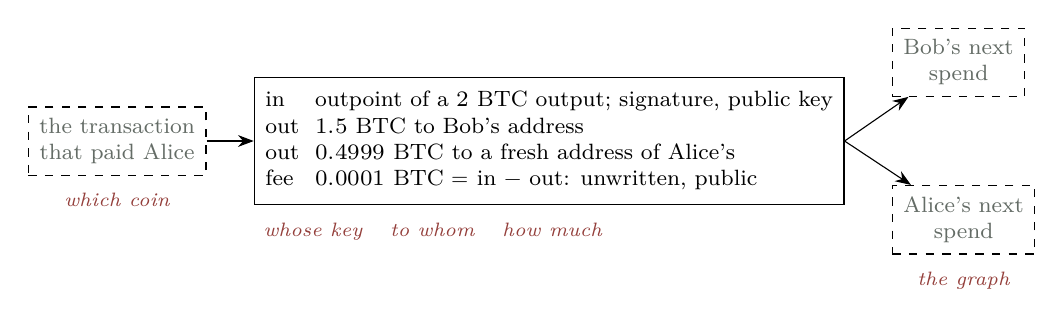
\begin{tikzpicture}[>={Stealth[length=2mm]}, font=\footnotesize,
  box/.style={draw, inner sep=4pt, align=left},
  ext/.style={draw, dashed, inner sep=4pt, align=center,
    text=arbdim},
  tag/.style={font=\scriptsize\itshape, text=arbred, align=center}]
\node[box] (tx) {\begin{tabular}{@{}l@{\ \ }l@{}}
  in  & outpoint of a $2$ BTC output; signature, public key \\
  out & $1.5$ BTC to Bob's address \\
  out & $0.4999$ BTC to a fresh address of Alice's \\
  fee & $0.0001$ BTC $=$ in $-$ out: unwritten, public \\
\end{tabular}};
\node[ext, left=6mm of tx] (prev) {the transaction\\ that paid Alice};
\node[ext, right=6mm of tx.east, yshift=10mm] (bobnext) {Bob's next\\ spend};
\node[ext, right=6mm of tx.east, yshift=-10mm] (alnext) {Alice's next\\ spend};
\draw[->] (prev) -- (tx);
\draw[->] (tx.east) -- (bobnext);
\draw[->] (tx.east) -- (alnext);
\node[tag, below=1mm of prev] {which coin};
\node[tag, below=1mm of alnext] {the graph};
\node[tag, below=1mm of tx.south west, anchor=north west]
  {whose key \quad to whom \quad how much};
\end{tikzpicture}}
\par\smallskip
\begin{itemize}
  \item Every output carries its spending condition and its amount; every
    input names an old output by identifier. Names cost outside
    information; the graph costs nothing.
  \item Reuse an address and its history merges; pay with change and the
    non-round output to a fresh address is usually yours. Both follow from
    the record, not from a careless wallet.
  \item The same shape --- one $2$-coin input, $1.5$ to Bob, change back
    --- returns as the shielded running example, with none of the labels.
\end{itemize}
\src{\emph{Ironwood Guide}, ``The four requirements on a shielded payment''}
\end{frame}

% a_checks.py:
%   (1) coin exists      Bitcoin: UTXO lookup
%   (2) authorised       Bitcoin: script + signature
%   (3) not spent twice  Bitcoin: UTXO deleted
%   (4) conserved        Bitcoin: sum(in) >= sum(out)
\begin{frame}{The validator's four checks}
{\ttfamily\small
\begin{tabular}{@{}l@{\qquad}l@{\qquad}l@{}}
validate(tx): & & \\
\quad for input in tx.inputs: & & \\
\quad\quad coin = utxo[input.prev\_out]
  & \normalfont (1) coin exists & \normalfont reads the outpoint \\
\quad\quad check sig(input.sig, coin.script)
  & \normalfont (2) authorised & \normalfont reads script and key \\
\quad\quad delete utxo[input.prev\_out]
  & \normalfont (3) not spent twice & \normalfont reads the outpoint \\
\quad check sum(in) >= sum(out)
  & \normalfont (4) conserved & \normalfont reads every amount \\
\end{tabular}}
\medskip
\begin{itemize}
  \item The whole state is one table, the set of unspent outputs; a spend
    is a lookup, a signature check, and a deletion.
  \item Every check reads a plaintext field of the transaction or of the
    output it names. Nothing is inferred; everything is looked at.
  \item The fee is the fourth check's slack, $\Sigma\,\mathrm{in} -
    \Sigma\,\mathrm{out}$: not a field, yet public to the satoshi.
\end{itemize}
\src{\emph{Ironwood Guide}, ``The four requirements on a shielded payment'';
  ``Resting: the note in the commitment tree''}
\end{frame}

% a_checks.py:
%   hide the amount           -> check(s) [4] die
%   hide the input reference  -> check(s) [1, 3] die
%   hide the key              -> check(s) [2] die
\begin{frame}{Hide a field, lose a check}
{\ttfamily\small
\begin{tabular}{@{}l@{\qquad}l@{}}
validate(tx): & \\
\quad for input in tx.inputs: & \\
\quad\quad \alert<3->{coin = utxo[input.prev\_out]}
  & \normalfont (1) coin exists \\
\quad\quad \alert<4->{check sig(input.sig, coin.script)}
  & \normalfont (2) authorised \\
\quad\quad \alert<3->{delete utxo[input.prev\_out]}
  & \normalfont (3) not spent twice \\
\quad \alert<2->{check sum(in) >= sum(out)}
  & \normalfont (4) conserved \\
\end{tabular}}
\medskip
\begin{itemize}
  \item<2-> \alert{Hide the amount}: check 4 dies --- nothing to add up.
  \item<3-> \alert{Hide the input reference}: checks 1 and 3 die ---
    nothing to look up, nothing to delete.
  \item<4-> \alert{Hide the key}: check 2 dies --- nothing to verify
    against.
  \item<5-> \alert{Hide the receiver}: nothing dies here --- the output's
    script is what check 2 reads when Bob spends it, so that spend's
    check 2 dies.
\end{itemize}
\medskip
\uncover<6->{Privacy, for this workshop: hide the sender, the receiver and
the amount, while a stranger still performs all four checks.}
\src{\emph{Ironwood Guide}, ``The four requirements on a shielded payment'';
  ``What a node verifies, without ever observing the note''}
\end{frame}

\begin{frame}{What a privacy design must supply}
\begin{center}\small\raggedright
\begin{tabular}{@{}p{0.31\textwidth}p{0.40\textwidth}p{0.23\textwidth}@{}}
\toprule
the validator must & the tool & Bitcoin's version \\
\midrule
accept a claim about data it cannot see & a zero-knowledge proof: the
  statement public, the witness (the prover's secret input, not
  Bitcoin's witness field) private & look at the data \\
know the hidden data cannot change under it & a commitment: hiding, and
  binding & the output, in the clear \\
notice the same hidden coin a second time & a nullifier: a keyed, one-way
  tag of the coin, published at spend & delete it from the set \\
add up amounts it cannot read & a homomorphic commitment: sealed
  envelopes that add & add the numbers \\
\bottomrule
\end{tabular}
\end{center}
\medskip
The proof checks the claim; the other three tools make the claim about
something fixed, unrepeatable, summable.
\src{\emph{Crypto Guide}, ``Three questions''; ``The sealed envelope'';
  \emph{Ironwood Guide}, ``The nullifier, and the loop back to minting''}
\end{frame}

% a_notes.py:
%   value range: 0 .. 2^64 - 1 = 18,446,744,073,709,551,615 zatoshi
\begin{frame}{Sealed envelopes that add}
The fourth tool in one line: two commitments add without either being
opened.
\[
\bigl([v_1]\,V + [r_1]\,R\bigr) + \bigl([v_2]\,V + [r_2]\,R\bigr)
  = [v_1 + v_2]\,V + [r_1 + r_2]\,R
\]
\begin{itemize}
  \item This is the Confidential Transactions trick: amounts hidden, their
    sum still checkable.
  \item It holds only modulo the group order; here the $64$-bit range check
    that closes the gap lives inside the proof.
\end{itemize}
\src{\emph{Crypto Guide}, ``The Pedersen commitment''; \emph{Ironwood
  Guide}, ``Conservation without disclosure: value commitments and the
  binding signature''; ``The Action statement, formally''}
\end{frame}

% a_notes.py:
%   value range: 0 .. 2^64 - 1 = 18,446,744,073,709,551,615 zatoshi
\begin{frame}{Notes versus UTXOs: what a coin is}
\begin{center}\small\raggedright
\begin{tabular}{@{}p{0.22\textwidth}p{0.31\textwidth}p{0.39\textwidth}@{}}
\toprule
 & Bitcoin UTXO & Zcash note \\
\midrule
owner & a script, usually one key hash, on chain & an address $(d, \pkd)$,
  inside the note \\
value & the amount, on chain & $v \in [0, 2^{64})$ zatoshi, inside the
  note \\
spending condition & script: signatures, timelocks, hashlocks & a key,
  full stop --- no script, no timelocks, no HTLCs \\
\bottomrule
\end{tabular}
\end{center}
\medskip
\begin{itemize}
  \item The owner and the value are fields of the note, and the note is
    never published; Bitcoin writes both on the output.
  \item Threshold authority exists (FROST, later) and is invisible on
    chain: one ordinary signature under one per-spend key.
\end{itemize}
\src{\emph{Ironwood Guide}, ``The note and its commitment''; ``Spend
  authorisation: RedPallas re-randomisation''; \emph{FROST Guide}, ``The
  three deployment surfaces''}
\end{frame}

% a_notes.py:
%   tree depth 32: 2^32 = 4,294,967,296 leaves
\begin{frame}{Notes versus UTXOs: what the chain records}
\begin{center}\small\raggedright
\begin{tabular}{@{}p{0.19\textwidth}p{0.31\textwidth}p{0.42\textwidth}@{}}
\toprule
 & Bitcoin UTXO & Zcash note \\
\midrule
on-chain identifier & the outpoint & a commitment $\cmsym$ to the note,
  stored as $\cmx$ \\
spent marker & removed from the UTXO set & a nullifier $\nfsym$,
  published at spend \\
set structure & one set: insert, delete & an append-only tree of $\cmx$,
  depth $32$, and a set of $\nfsym$: append only, both \\
\bottomrule
\end{tabular}
\end{center}
\medskip
The note never touches the chain: recorded are a commitment to it, an
encrypted copy for its recipient, and at spend a tag derived from it.
\src{\emph{Ironwood Guide}, ``The note and its commitment''; ``The tree, its
  hash, and its anchors''; ``The nullifier, and the loop back to minting''}
\end{frame}

\begin{frame}{The three-line mental model}
A shielded spend is three claims about a note nobody sees:
\begin{enumerate}
  \item \emph{it exists} --- a commitment to it is a leaf under a public
    root, proved with leaf, position and path all private;
  \item \emph{it is spent now} --- its serial number, the nullifier, is
    revealed, and the chain refuses to see it twice;
  \item \emph{the books balance} --- commitments to the amounts add up to
    the declared net flow.
\end{enumerate}
\[
R_{\mathrm{mem}} = \bigl\{\, (\underbrace{\mathit{rt}}_{\text{public}};\
  \underbrace{(\cmx,\ i,\ \mathit{path})}_{\text{private}}) \ :\
  \mathsf{Verify}(\mathit{rt}, i, \cmx, \mathit{path}) = \mathsf{accept}
  \,\bigr\}
\]
A Bitcoin spend names its coin and signs. A shielded spend names nothing:
it proves the first line, reveals the second, and signs for the third ---
and, as in Bitcoin, the spender signs, under a key the proof ties to the
note (check 2). Everything else in the workshop is machinery for these
three and for that signature.
\src{\emph{Crypto Guide}, ``Privacy-preserving membership via zero-knowledge
  paths''; ``A shielded spend, end to end''; \emph{Ironwood Guide},
  ``Conservation without disclosure: value commitments and the binding
  signature''}
\end{frame}

% a_checks.py:
%   (1) coin exists      shielded: commitment in an append-only tree +
%                                  membership proof (A3)
%   (2) authorised       shielded: key knowledge in the circuit (A6/A7) +
%                                  re-randomised signature
%   (3) not spent twice  shielded: nullifier, published once, in the
%                                  nullifier set (A5)
%   (4) conserved        shielded: homomorphic value commitments (A4) +
%                                  binding signature
\begin{frame}{Four checks, four mechanisms}
\begin{center}\small
\begin{tabular}{@{}clp{0.26\textwidth}p{0.42\textwidth}@{}}
\toprule
 & the check & Bitcoin & shielded Zcash \\
\midrule
(1) & coin exists & look the outpoint up in the UTXO set & a commitment
  in an append-only tree; a membership proof under a public root \\
(3) & not spent twice & delete it from the set & a nullifier, published
  once, refused the second time \\
(4) & conserved & add the amounts up & value commitments that add; a
  binding signature over their sum \\
(2) & authorised & run the script over the signature & key knowledge
  proved inside the proof; a signature under a re-randomised key \\
\bottomrule
\end{tabular}
\end{center}
\medskip
Each right-hand cell names what replaces one Bitcoin check; why the
Bitcoin way is gone was settled on \emph{Hide a field, lose a check}. Each
part of the workshop reopens with both questions.
\src{\emph{Ironwood Guide}, ``The four requirements on a shielded payment'';
  ``The Action statement, formally''}
\end{frame}

\begin{frame}{The route}
\begin{enumerate}
  \item \textbf{The toolbox} --- each primitive from the Bitcoin instance
    the room already holds.
  \item \textbf{The data model} --- notes, commitments, the tree, the
    nullifier: checks 1 and 3.
  \item \textbf{Keys and addresses} --- who can spend, who can see.
  \item \textbf{The Action statement} --- what the proof proves, clause by
    clause; then a break.
  \item \textbf{Balance and authority} --- checks 4 and 2, on the running
    example.
  \item \textbf{The proof system} --- from a statement to a few kilobytes.
  \item \textbf{Delivery and light clients} --- how Bob finds his money.
  \item \textbf{The transaction and the turnstile} --- the bytes on the
    chain, and the pools.
  \item \textbf{Consensus} --- why one fork wins, what the chain must
    remember.
  \item \textbf{Limits, frontier, takeaways.}
\end{enumerate}
\medskip
One example threads it: Alice pays Bob $1.5$ ZEC from a $2$ ZEC note.
\end{frame}

% a_checks.py: nullifier serves check 3
\begin{frame}{Checkpoint}
{\large Which of the four checks does a nullifier serve, and what breaks if
two different notes could share one?}
\pause
\medskip
\begin{itemize}
  \item Check 3, not spent twice. The nullifier is ``delete from the UTXO
    set'' without naming the coin: published once, refused the second
    time.
  \item Two notes, one nullifier: whichever is spent first burns the other,
    and the second owner's honest spend is refused as a double spend ---
    an attack on earlier designs, in which forged notes could be made to
    share one.
  \item How the chain makes sure no two accepted notes can share one ---
    every new note inherits, as its seed, the serial of the note spent
    beside it --- is Part C's business.
\end{itemize}
\src{\emph{Ironwood Guide}, ``The nullifier, and the loop back to minting''}
\end{frame}

%% ---- 02-toolbox.tex
%% Part B --- The toolbox, from Bitcoin's primitives up.
%% Frames only. Numbers: compute/b_primitives.py, b_proofsizes.py,
%% g_twoadic.py, a_proofsizes.py, e_tree.py (outputs pasted above each
%% frame). No shared figure macros are defined or used here.

\newcommand{\Bahead}[1]{{\small\textcolor{arbdim}{\emph{Ahead:} #1}}}
\newcommand{\Bpers}[1]{\ensuremath{\text{``}\mathtt{#1}\text{''}}}

\divider{Part B}{The toolbox, from Bitcoin's primitives up}

%% ---------------------------------------------------------------- B1
% b_primitives.py:
%   256-bit digest: generic collision ~ 2^128, preimage ~ 2^256
%   160-bit digest: generic collision ~ 2^80, preimage ~ 2^160
\begin{frame}{Hash functions: one primitive, three notions}
A fixed public function $H \colon \{0,1\}^{*} \to \{0,1\}^{n}$ that
compresses.
\begin{itemize}
  \item \emph{Preimage resistance}: given $y$, no efficient adversary finds
    any $x'$ with $H(x') = y$.
  \item \emph{Second-preimage resistance}: given $x$, none finds
    $x' \ne x$ colliding with it.
  \item \emph{Collision resistance}: none finds any pair $x \ne x'$ with
    $H(x) = H(x')$. The adversary picks both, so this is the strongest
    demand --- and the one commitments, Merkle trees and Fiat--Shamir need.
  \item Generic cost: a collision after about $2^{n/2}$ evaluations (the
    birthday bound), a preimage after $2^{n}$. Hence $256$-bit digests for
    $128$-bit collision security; RIPEMD-160 sits at $2^{80}$.
\end{itemize}
\medskip
\begin{itemize}
  \item Bitcoin: SHA-256d over block headers and every txid;
    $\mathsf{hash160} = \mathrm{RIPEMD160} \circ \mathrm{SHA256}$ inside
    addresses.
  \item Zcash keeps every one of those in its transparent layer, and adds
    three hashes for the shielded one.
\end{itemize}
\src{\emph{Crypto Guide}, ``Security notions: preimage, second-preimage,
  and collision resistance''; ``The birthday bound on generic collision
  finding''; ``The transparent layer's hashes''}
\end{frame}

% b_primitives.py:
%   Poseidon: t = 3 (rate 2, capacity 1), S-box x^5, 8 full + 56 partial
%     = 64 rounds
%   Sinsemilla: k = 10-bit chunks, table 2^10 = 1024 points + Q; per chunk
%     1 lookup + 2 incomplete additions
\begin{frame}{Zcash's hashes: SHA-256 is not replaced}
\begin{center}\small
\begin{tabular}{@{}lp{0.3\textwidth}p{0.45\textwidth}@{}}
\toprule
hash & kind & deployed use \\
\midrule
SHA-256d & \raggedright bit-oriented, Bitcoin's & \raggedright header
  difficulty filter (after Equihash); transparent layer: legacy txids,
  Base58Check \tabularnewline
BLAKE2b & \raggedright bit-oriented; personalised natively, the key
  prepended to the input &
  \raggedright $\mathsf{PRFexpand}$ (the key tree); note-encryption KDF;
  ZIP-244 digests (txid, sighash) \tabularnewline
Poseidon & \raggedright algebraic: $x \mapsto x^{5}$ over $\Fpp$ &
  \raggedright the nullifier PRF, inside the circuit \tabularnewline
Sinsemilla & \raggedright algebraic: curve additions on \Pallas{} &
  \raggedright note commitment; Merkle node hash --- both inside the
  circuit \tabularnewline
\bottomrule
\end{tabular}
\end{center}
\smallskip
Bitcoin's hashes stay where Bitcoin put them; the shielded protocol adds
one bit-oriented hash for work off the circuit, two algebraic ones for work
inside it.
\par\smallskip
\Bahead{Poseidon and Sinsemilla in Part C; BLAKE2b in Parts D, F and H.}
\src{\emph{Consensus Guide}, ``Equihash and the memoryless model'';
  \emph{Crypto Guide}, ``The transparent layer's hashes''; ``PRFs from hash
  functions: length extension and keyed BLAKE2''; ``Arithmetisation-friendly
  hashing: Poseidon''; \emph{Ironwood Guide}, ``Sinsemilla: hash,
  commitment, and short forms''}
\end{frame}

% b_primitives.py:
%   Poseidon: t = 3 (rate 2, capacity 1), S-box x^5, 8 full + 56 partial
%     = 64 rounds
%   Sinsemilla: k = 10-bit chunks, table 2^10 = 1024 points + Q; per chunk
%     1 lookup + 2 incomplete additions
\begin{frame}{Why in-circuit hashing wants algebraic hashes}
\begin{itemize}
  \item A zero-knowledge proof re-expresses every step of a computation as
    polynomial constraints over a prime field; a field multiplication is
    one constraint, a Boolean operation is several plus range checks.
  \item SHA-256 and BLAKE2 shuffle and XOR $32$- and $64$-bit words:
    foreign to the field, tens of thousands of constraints per evaluation.
  \item Poseidon: the round is add constants, raise the state to $x^{5}$
    (every element in a full round, one element in a partial round),
    multiply by a fixed matrix; the only non-linear step is $x^{5}$. A
    $2$-to-$1$ hash costs a few hundred constraints. Orchard's instance:
    state width $3$, $8$ full and $56$ partial rounds.
  \item Sinsemilla: per $10$-bit chunk, one lookup into a table of
    $2^{10} = 1024$ hashed-to-curve points and two incomplete curve
    additions --- native operations, and collision resistance that reduces
    to the discrete logarithm.
  \item Bitcoin never hashes inside a proof; the first shielded generation
    did, with SHA-256, and its prover paid for it.
\end{itemize}
\src{\emph{Crypto Guide}, ``Arithmetisation-friendly hashing: Poseidon'';
  ``Sinsemilla: an algebraic hash-based commitment''; \emph{Ironwood Guide},
  ``Why Sinsemilla: in-circuit cost''; ``Lineage: three generations of
  shielded proof''}
\end{frame}

%% ---------------------------------------------------------------- B2
% b_primitives.py: secp256k1 p = 2^256 - 2^32 - 977, 256 bits
% g_twoadic.py: Pallas base field bits = 255; Vesta base field bits = 255
\begin{frame}{Curves: the same shape, different primes}
Short Weierstrass $y^{2} = x^{3} + b$ over a prime field; the points form a
group of prime order, cofactor $1$; the discrete logarithm in it is the
standing assumption.
\begin{itemize}
  \item Bitcoin: secp256k1, $b = 7$ over $p = 2^{256} - 2^{32} - 977$, a
    $256$-bit prime order. The audience's keys, ECDSA and BIP-340 live here.
  \item Zcash: \Pallas{} and \Vesta{}, $b = 5$ over two $255$-bit primes
    $p_{\Pallas}$, $p_{\Vesta}$, with $\#\Pallas = p_{\Vesta}$ and
    $\#\Vesta = p_{\Pallas}$: the scalar field of each is the base field of
    the other. About $126$ bits of discrete-log security.
  \item Every Pallas and Vesta generator the protocol uses is hashed to
    the curve (secp256k1's base point is a SEC~2 constant): no relation
    between any two is known to anyone, and no ceremony for this stack
    (the Sapling pool still rests on its Groth16 MPC, Part G).
  \item Pallas carries every point in an Action --- commitments, nullifier
    base, keys, ephemeral keys, signatures; Vesta carries the proof's
    polynomial commitments.
\end{itemize}
\Bahead{the division of labour between the two curves in Part G.}
\src{\emph{Crypto Guide}, ``Instantiation on elliptic curves; the Pasta
  curves''; ``The transparent layer's schemes: ECDSA and BIP-340 over
  secp256k1''; \emph{Math Guide}, ``Pallas and Vesta assembled''}
\end{frame}

% g_twoadic.py:
%   Pallas base field        bits = 255  two-adicity(p-1) = 32
%     largest 2^k domain = 2^32  hosts 2^11 rows: True
%   Vesta base field         bits = 255  two-adicity(p-1) = 32
%     largest 2^k domain = 2^32  hosts 2^11 rows: True
%   secp256k1 base field     bits = 256  two-adicity(p-1) =  1
%     largest 2^k domain = 2^1 = 2  hosts 2^11 rows: False
%   secp256k1 scalar field   bits = 256  two-adicity(p-1) =  6
%     largest 2^k domain = 2^6 = 64  hosts 2^11 rows: False
\begin{frame}{Why not secp256k1: two-adicity}
A proof system of the PLONK family interpolates each circuit column over
the $2^{k}$-th roots of unity of its field. Those exist iff
$2^{k} \mid p - 1$; the largest such $k$ is the field's \emph{two-adicity}.
\begin{center}\small
\begin{tabular}{@{}lccl@{}}
\toprule
field & bits & two-adicity of $p - 1$ & largest power-of-two domain \\
\midrule
\Pallas{} base field & $255$ & $32$ & $2^{32}$ \\
\Vesta{} base field & $255$ & $32$ & $2^{32}$ \\
secp256k1 base field & $256$ & $1$ & $2$ \\
secp256k1 scalar field & $256$ & $6$ & $64$ \\
\bottomrule
\end{tabular}
\end{center}
\begin{itemize}
  \item The Orchard circuit has $2^{11}$ rows; neither secp256k1 field
    offers a domain of that size. The Pasta primes were searched for with
    two-adicity $32$ and the cycle as design goals.
  \item The secp256k1 rows are the deck's own computation, not a volume
    figure.
\end{itemize}
\Bahead{rows, roots of unity and the polynomial identity in Part G.}
\src{\emph{Math Guide}, ``Roots of unity and evaluation domains'', Remark
  ``Two-adicity and FFT-friendly primes''; ``Base fields, scalar fields, and
  the Pasta cycle''; \emph{Crypto Guide}, ``The transparent layer's schemes:
  ECDSA and BIP-340 over secp256k1''}
\end{frame}

%% ---------------------------------------------------------------- B3
% (no numbers)
\begin{frame}{Commitments: a sealed envelope}
A commitment $c = \Comm(m; r)$ with a random trapdoor $r$: \emph{hiding}
--- from $c$, two candidate messages are indistinguishable; \emph{binding}
--- no $c$ opens to two messages. The two cannot both be perfect; the
deployed schemes are perfectly hiding, binding under the discrete logarithm.
\smallskip
The Pedersen commitment on \Pallas{}, with $V, R$ hashed to the curve:
\[
  \Comm(v; r) := [v]\,V + [r]\,R .
\]
For uniform $r$ the point is uniform whatever $v$ is; two openings of one
$c$ solve $\log_{V} R$, which nobody holds.
\begin{itemize}
  \item Bitcoin: this envelope is Confidential Transactions'; an address is
    a hash commitment to a public key or a script, opened at spend.
  \item Zcash: $\cvsym$ seals an Action's value change (Pedersen, so it
    adds); $\cmsym$ seals a whole note --- an algebraic hash plus a
    blinding term $[\rcm]\,H_{D}$ of the same Pedersen shape, over its own
    hashed generator, so the circuit recomputes it cheaply.
\end{itemize}
\src{\emph{Crypto Guide}, ``Hiding and binding''; ``The Pedersen
  commitment''; ``Sinsemilla: an algebraic hash-based commitment'';
  \emph{Ironwood Guide}, ``Sinsemilla: hash, commitment, and short forms''}
\end{frame}

% b_primitives.py: note value: 0 .. 2^64 - 1
\begin{frame}{The envelope adds: the Confidential Transactions bridge}
\[
  \Comm(v_{1}; r_{1}) + \Comm(v_{2}; r_{2})
  = \Comm(v_{1} + v_{2};\ r_{1} + r_{2}),
\]
so, for a set of inputs and outputs,
\[
  \sum \Comm_{\mathrm{in}} - \sum \Comm_{\mathrm{out}}
  = \Bigl[\sum v_{\mathrm{in}} - \sum v_{\mathrm{out}}\Bigr] V
    + [\bar r]\,R ,
\]
and the $V$ term vanishes exactly when the values balance --- modulo the
group order. A range check on every value closes the wrap.
\begin{itemize}
  \item Confidential Transactions (Elements): the same equation on the
    chain; a range proof beside each commitment; the receiver is told the
    opening. Amounts hidden, keys and graph in the clear.
  \item Here: the $64$-bit range check and the opening $(v, \rcv)$ are
    clauses of one zero-knowledge proof, alongside the sender's
    authorisation and the receiver's note; the net trapdoor $\bar r$
    becomes a signing key.
\end{itemize}
\Bahead{clause A4 in Part E; the balance walk-through in Part E$'$.}
\src{\emph{Crypto Guide}, ``The Pedersen commitment''; ``Binding signatures
  as a proof of knowledge of a discrete logarithm''}
\end{frame}

%% ---------------------------------------------------------------- B4
% e_tree.py: depth 32: 2^32 = 4294967296 leaves; path = 32 siblings
% b_primitives.py: tree depth 32: path = 32 siblings + 32 direction bits
\begin{frame}{Merkle trees: from the txid tree to the note commitment tree}
\begin{columns}[c]
\begin{column}{0.56\textwidth}
\begin{itemize}
  \item Bitcoin: each block hashes its txids pairwise up to a root in the
    header; an SPV proof is the leaf plus one sibling per level, and the
    leaf --- the txid --- is public.
  \item Zcash: the leaves are $\cmx$ in creation order; depth $32$, room
    for $2^{32}$ notes; the node hash is Sinsemilla, tagged with its layer;
    the root after each block is that block's \emph{anchor}.
  \item A membership proof: $32$ siblings and $32$ direction bits, verified
    by $32$ hashes --- recomputed here inside the proof.
\end{itemize}
\end{column}
\begin{column}{0.42\textwidth}
\centering
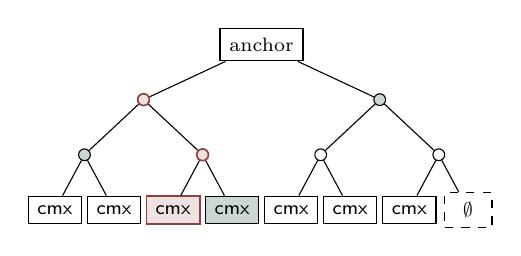
\begin{tikzpicture}[every node/.style={font=\scriptsize},level distance=7mm,
  level 1/.style={sibling distance=30mm},
  level 2/.style={sibling distance=15mm},
  level 3/.style={sibling distance=7.5mm},
  nd/.style={draw,circle,inner sep=1.5pt},
  lf/.style={draw,minimum width=6mm},
  rt/.style={draw=arbred,thick,fill=arbred!15},
  sb/.style={fill=arb!25}]
\node[draw,thick] {anchor}
  child {node[nd,rt] {}
    child {node[nd,sb] {}
      child {node[lf] {\cmx}}
      child {node[lf] {\cmx}}}
    child {node[nd,rt] {}
      child {node[lf,rt] {\cmx}}
      child {node[lf,sb] {\cmx}}}}
  child {node[nd,sb] {}
    child {node[nd] {}
      child {node[lf] {\cmx}}
      child {node[lf] {\cmx}}}
    child {node[nd] {}
      child {node[lf] {\cmx}}
      child {node[lf,dashed] {$\varnothing$}}}};
\end{tikzpicture}
\par
{\scriptsize red: the leaf and its route, private; green: the siblings,
private; the anchor alone is public}
\end{column}
\end{columns}
\src{\emph{Crypto Guide}, ``Authentication paths and membership proofs'';
  \emph{Ironwood Guide}, ``The tree, its hash, and its anchors''}
\end{frame}

% e_tree.py: depth 32: path = 32 siblings
\begin{frame}{What changes: append only, historical roots, private path}
\begin{itemize}
  \item \emph{Append only.} One leaf at a time; the \emph{frontier} --- at
    most $32$ carried labels --- updates the root in $32$ hashes. Nothing
    is ever deleted; the ``deleted'' half of the state is a separate set.
  \item \emph{History binding.} A proof formed against the root at
    insertion stays valid against that root forever, and consensus accepts
    the anchor of any earlier main-chain block.
  \item \emph{Private path.} Revealing (leaf, index, siblings) would say
    which note is spent; so the path is a witness of the zero-knowledge
    proof and only the anchor is a statement:
    \[
      R_{\mathrm{mem}} = \bigl\{\,(\mathit{rt};\ (\cmx, i, \mathit{path})) :
        \mathsf{Verify}(\mathit{rt}, i, \cmx, \mathit{path})
        = \mathsf{accept}\,\bigr\}.
    \]
  \item Bitcoin contrast: an SPV proof names the txid it proves; this proof
    names only the root, and hides the leaf among every leaf beneath it.
\end{itemize}
\Bahead{the tree, anchors and the nullifier set in Part C; clause A3 in
  Part E.}
\src{\emph{Crypto Guide}, ``Append-only and incrementally updatable trees'';
  ``Privacy-preserving membership via zero-knowledge paths'';
  \emph{Ironwood Guide}, ``The tree, its hash, and its anchors''}
\end{frame}

%% ---------------------------------------------------------------- B5
% b_primitives.py:
%   Poseidon: t = 3 (rate 2, capacity 1), S-box x^5, 8 full + 56 partial
%     = 64 rounds
\begin{frame}{Pseudorandom functions: a key that fakes randomness}
A keyed function $F_{k}$ is \emph{pseudorandom} if, for a secret uniform
$k$, no efficient adversary with oracle access --- any inputs, adaptively
--- tells $F_{k}$ from a truly random function.
\begin{itemize}
  \item The algorithm is public; only $k$ is hidden. The adversary never
    sees $k$, only input--output pairs of her choosing.
  \item Bitcoin: HMAC-SHA512 inside BIP-32 child derivation --- a PRF the
    audience already trusts to make child keys look unrelated.
  \item Zcash, off the circuit: BLAKE2b, personalised, as
    $\mathsf{PRFexpand}$ --- one call per sub-secret,
    $\mathsf{sk} \to \asksym, \nksym, \rivk$, and later the note's
    randomness from its seed.
  \item Zcash, inside the circuit: Poseidon over $\Fpp$, keyed by its first
    input,
    \[
      F_{\nksym}(\rho) = \mathsf{PoseidonHash}(\nksym, \rho),
    \]
    state width $3$, S-box $x^{5}$, $8$ full and $56$ partial rounds.
\end{itemize}
\Bahead{$\mathsf{PRFexpand}$ builds the key ladder in Part D.}
\src{\emph{Crypto Guide}, ``Pseudorandom functions and permutations'';
  ``PRFs from hash functions: length extension and keyed BLAKE2'';
  ``Arithmetisation-friendly hashing: Poseidon''}
\end{frame}

% (no numbers)
\begin{frame}{What a nullifier needs from a PRF}
The nullifier, previewed:
\[
  \nfsym = \Extract\bigl([\,F_{\nksym}(\rho) + \psi\,]\,G^{\mathsf{nf}}
    + \cmsym\bigr).
\]
{\small $\Extract$: the $x$-coordinate; $\rho, \psi$: per-note randomness
fixed at creation (Part C); $G^{\mathsf{nf}}$: a hashed generator.}
\par\smallskip
Two properties, and they are separate:
\begin{itemize}
  \item \emph{Uniqueness}: every input ($\nksym$, $\rho$, $\psi$,
    $\cmsym$) is fixed once the note exists, so the tag is deterministic;
    two distinct notes sharing a tag yield a discrete-log relation on
    \Pallas{}. No PRF property is used here --- the forger holds
    $\nksym$.
  \item \emph{Unlinkability}: without $\nksym$ the term
    $[F_{\nksym}(\rho) + \psi]\,G^{\mathsf{nf}}$ masks $\cmsym$ with a
    value that looks random --- by Poseidon's PRF security or,
    independently, by DDH on \Pallas{}. Either assumption suffices.
  \item Bitcoin contrast: the spent marker is the outpoint itself, unique
    and public; a nullifier must be unique \emph{and} say nothing.
\end{itemize}
\Bahead{the nullifier in full in Part C; clause A5 in Part E.}
\src{\emph{Ironwood Guide}, ``The nullifier, and the loop back to
  minting''; ``Nullifier uniqueness''}
\end{frame}

%% ---------------------------------------------------------------- B6
% (no numbers)
\begin{frame}{Key agreement: the ECDH of silent payments}
On a prime-order curve with base point $P$: a secret $a$, a public $[a]P$,
and $\mathrm{Agree}(a, Q) = [a]Q$, so that $[a]([b]P) = [b]([a]P)$.
\begin{itemize}
  \item Bitcoin (BIP-352): the sender's input key and the receiver's scan
    key agree on a secret that tweaks the output key. Nothing is encrypted;
    the receiver scans for outputs that decode under the shared secret.
  \item Zcash: the address carries a static key $\pkd = [\ivk]\,\gd$ over
    a per-address base $\gd$, itself hashed from the diversifier. The
    sender draws an ephemeral $\esk$ (from the note's seed, by
    $\mathsf{PRFexpand}$) and publishes $\epk = [\esk]\,\gd$:
    \[
      \mathsf{s} = [\esk]\,\pkd = [\ivk]\,\epk .
    \]
  \item Static--ephemeral: the recipient was never online, and the sender
    learns nothing beyond the address. Cofactor $1$ leaves only the
    on-curve, non-identity check on $\epk$.
\end{itemize}
\Bahead{note encryption step by step in Part F.}
\src{\emph{Crypto Guide}, ``Elliptic-curve Diffie--Hellman'';
  ``Shielded-note delivery as deployed hybrid encryption'';
  \emph{Ironwood Guide}, ``Sender: one-shot Diffie--Hellman and the AEAD''}
\end{frame}

% b_primitives.py:
%   ChaCha20-Poly1305: 256-bit key, 96-bit nonce (all zero), 128-bit tag;
%     wrong-key acceptance ~ 2^-128
\begin{frame}{Encryption on top: KDF, AEAD, wrong-key rejection}
\begin{itemize}
  \item \emph{KDF}: one personalised hash call,
    $K_{\mathrm{enc}} = \mathrm{BLAKE2b}\text{-}256\bigl(
      \Bpers{Zcash\_OrchardKDF};\ \mathsf{s} \,\|\, \epk\bigr)$; folding
    $\epk$ in binds the key to this ephemeral.
  \item \emph{AEAD}: ChaCha20-Poly1305 under the $256$-bit key, nonce all
    zero and associated data empty --- safe because each key encrypts
    exactly once --- with a $128$-bit tag.
  \item \emph{Wrong-key rejection}: decryption under an independent key
    returns $\bot$ except with probability about $2^{-128}$. This is what
    lets a wallet try every output on the chain with its own key. The
    scheme is not key-committing, so the wallet also recomputes $\cmsym$
    from the plaintext and compares.
  \item Bitcoin never encrypts anything on chain: scripts and amounts are
    plaintext by design. Here the recipient, the value and the memo exist
    on chain only inside the ciphertext.
  \item Two ciphertexts per Action: one to the recipient, one to the
    sender's own outgoing key.
\end{itemize}
\Bahead{trial decryption and compact blocks in Part F.}
\src{\emph{Crypto Guide}, ``Key-derivation functions''; ``The
  ChaCha20-Poly1305 AEAD''; \emph{Ironwood Guide}, ``Sender: one-shot
  Diffie--Hellman and the AEAD''}
\end{frame}

%% ---------------------------------------------------------------- B7
% b_primitives.py: RedPallas nonce randomiser: 80 bytes; hash BLAKE2b-512
\begin{frame}{Signatures: ECDSA, Schnorr, RedPallas}
\begin{itemize}
  \item Bitcoin: ECDSA $(r, s)$ over secp256k1, DER plus a sighash-type
    byte; under Taproot, BIP-340 Schnorr, $s = k + e\,d$ with
    $e = H(x(R) \,\|\, x(X) \,\|\, m)$.
  \item Zcash, transparent: the same ECDSA (sighash as message, DER,
    low-$s$). No Taproot, no BIP-340 in the transparent layer.
  \item Zcash, shielded: \emph{RedPallas} --- Schnorr over \Pallas{} with
    the base point $P$ a parameter of the scheme. Keys $X = [x]P$;
    \begin{align*}
      \text{Sign:}\quad & r = H(T \,\|\, X \,\|\, m)\ \text{for $80$ fresh
        random bytes $T$},\ R = [r]P, \\
      & c = H(R \,\|\, X \,\|\, m),\quad s = r + c\,x ; \\
      \text{Verify:}\quad & [s]P = R + [c]X ,
    \end{align*}
    with $H$ BLAKE2b-512, personalised, reduced modulo the group order.
  \item Two instantiations, differing only in $P$: the spend-authorisation
    base $G^{\mathsf{SpendAuth}}$, and the value-commitment base $R$.
\end{itemize}
\src{\emph{Crypto Guide}, ``The transparent layer's schemes: ECDSA and
  BIP-340 over secp256k1''; ``RedDSA: re-randomisable Schnorr for
  Orchard''}
\end{frame}

% (no numbers)
\begin{frame}{The need: one spend key per wallet, not per coin}
\begin{itemize}
  \item Bitcoin: one key per output. Reuse is a wallet's choice, and each
    reuse links two payments.
  \item Zcash: one spend validating key per wallet,
    $\aksym = [\asksym]\,G^{\mathsf{SpendAuth}}$, and every diversified
    address shares it:
    \[
      \ivk = \CommitIvk_{\rivk}\bigl(\Extract(\aksym), \nksym\bigr),
      \qquad \pkd = [\ivk]\,\gd .
    \]
  \item An un-randomised spend would publish $\aksym$ --- the same key for
    every note the wallet ever spends. Linkage worse than address reuse,
    and structural rather than chosen.
  \item Hence a fresh disguise per spend. The public key must be shiftable
    without the secret; a Schnorr key is the homomorphic image $[x]P$ of
    its secret, so it can be.
\end{itemize}
\Bahead{the ladder that makes every address share $\aksym$ in Part D.}
\src{\emph{Crypto Guide}, ``Key re-randomisation and unlinkability'';
  \emph{Ironwood Guide}, ``Viewing keys''; ``Diversified addresses''}
\end{frame}

% (no numbers)
\begin{frame}{Key re-randomisation, additive}
For a fresh uniform $\alpha$ per spend --- added, never multiplied in:
\[
  \rsk := \asksym + \alpha, \qquad
  \rksym := \aksym + [\alpha]\,G^{\mathsf{SpendAuth}}
    = [\rsk]\,G^{\mathsf{SpendAuth}} .
\]
\begin{itemize}
  \item \emph{Consistency}: $(\rsk, \rksym)$ is an ordinary key pair; a
    signature under $\rsk$ verifies under $\rksym$.
  \item \emph{Unlinkability}: for uniform $\alpha$ the key $\rksym$ is
    uniform on the group whatever $\aksym$ is --- perfect, no assumption,
    provided $\alpha$ is fresh and stays secret.
  \item Signing under $\rksym$ needs both $\asksym$ and $\alpha$. The
    circuit proves $\rksym$ is a re-randomisation of the $\aksym$ bound
    into the note's address; the node checks the signature under $\rksym$.
  \item Bitcoin bridge: a non-hardened BIP-32 child is
    $\text{pubkey} + [\text{tweak}]\,G$ too --- but anyone holding the
    parent xpub (key, chain code, index) recomputes its tweak; this one is
    uniform and never published.
\end{itemize}
\Bahead{clauses A6/A7 in Part E; the signature on the wire in Part E$'$.}
\src{\emph{Crypto Guide}, ``Key re-randomisation and unlinkability'';
  \emph{Ironwood Guide}, ``Spend authorisation: RedPallas
  re-randomisation''}
\end{frame}

% (no numbers)
\begin{frame}{Preview: a signature under a key nobody holds unless the
  values balance}
\small
\setlength{\abovedisplayskip}{3pt}\setlength{\belowdisplayskip}{3pt}
Sum the Actions' value commitments and fold in the public balance:
\[
  \mathsf{bvk} = \sum \cvsym - [\mathsf{valueBalance}]\,V
  \quad\text{(public)}.
\]
\begin{itemize}
  \item Every group element is some multiple of $R$; what matters is who
    can compute the multiplier. If the hidden values balance, the $V$ terms
    cancel, $\mathsf{bvk} = [\sum \rcv]\,R$, and the author knows
    $\mathsf{bsk} = \sum \rcv$. If not, writing $\mathsf{bvk}$ as any
    multiple $[\beta]\,R$ would reveal $\log_{R} V$, which nobody holds.
  \item The \emph{binding signature}: RedPallas under $\mathsf{bsk}$,
    verified under $\mathsf{bvk}$, over the sighash. A Schnorr signature
    proves knowledge of a discrete logarithm; here knowing it means ``the
    values balance''. Range checks in the proof lift balance modulo the
    group order to balance over the integers.
  \item Bitcoin's check 4 reads the amounts; here they stay sealed and a
    signature certifies their sum.
\end{itemize}
\Bahead{the running example's balance, in a toy group, in Part E$'$.}
\src{\emph{Crypto Guide}, ``Binding signatures as a proof of knowledge of a
  discrete logarithm''}
\end{frame}

%% ---------------------------------------------------------------- B8
% (no numbers)
\begin{frame}{Zero-knowledge proofs, first contact}
A relation $R$ of pairs $(x, w)$: the \emph{statement} $x$ is public, the
\emph{witness} $w$ private; the claim is ``I know $w$ with
$(x, w) \in R$''.
\begin{itemize}
  \item \emph{Complete}: an honest prover holding $w$ convinces.
  \item \emph{Sound}: no prover convinces on a false $x$ --- an
    \emph{argument} if only efficient provers are excluded, the price of
    succinctness.
  \item \emph{Zero knowledge}: a simulator without $w$ reproduces the
    verifier's whole view; nothing beyond $x$ leaks.
  \item \emph{Knowledge sound}: whoever convinces can be rewound into
    surrendering $w$. Needed here: ``some spendable note exists in the
    tree'' is true for everyone; ``I hold one'' is the claim.
\end{itemize}
\src{\emph{Crypto Guide}, ``Languages, relations, and witnesses'';
  ``Interactive protocols, proofs, and arguments''; ``Knowledge soundness
  and extractors''; ``The simulation paradigm and zero knowledge''}
\end{frame}

% (no numbers)
\begin{frame}{A signature on a statement}
\begin{itemize}
  \item Interaction removed by Fiat--Shamir: each challenge becomes a hash
    of the statement and the transcript so far, so one string carries the
    whole exchange and anyone can re-derive the challenges.
  \item Proof of knowledge $+$ Fiat--Shamir $=$ signature. The audience's
    Schnorr signature is exactly this: a proof of knowledge of $x$ in
    $X = [x]G$, with the message folded into the challenge hash.
  \item Bitcoin verifies one equation per signature; this verifier runs
    one fixed circuit's verifying key against the statement, per proof.
\end{itemize}
\src{\emph{Crypto Guide}, ``The Fiat--Shamir transform: from interactive to
  non-interactive''; ``SNARKs: succinct non-interactive arguments of
  knowledge''}
\end{frame}

% (no numbers)
\begin{frame}{A SNARK: succinct, hence an argument}
\begin{itemize}
  \item A SNARK is the same move on a whole statement --- ``this note is in
    the tree, this nullifier is its, these values balance'' --- with the
    proof size and the verifier's time sublinear in the computation.
  \item Halo 2, as deployed: the proof is; the verifier's linear part is
    shared across a batch of proofs (Part G).
  \item Succinctness forces an \emph{argument}: a proof shorter than the
    witness cannot pin the witness down against an unbounded prover, so
    soundness holds against efficient provers, under an assumption.
\end{itemize}
\Bahead{the statement in Part E; the proof system in Part G.}
\src{\emph{Crypto Guide}, ``SNARKs: succinct non-interactive arguments of
  knowledge''; \emph{Ironwood Guide}, ``Comparative summary''}
\end{frame}

% b_proofsizes.py:
%   Sprout  BCTV14  per JoinSplit            296 B
%   Sapling Groth16 per Spend / per Output   192 B
%   Orchard Halo 2  per bundle 2720 + 2272*a  a=1: 4992 B
%   running example (1 spend, 2 outputs):
%     Sprout   1 JoinSplit           = 296 B
%     Sapling  3 descriptions      = 576 B
%     Ironwood 2 Actions, one proof = 7264 B
\begin{frame}{Proof sizes, with units}
\begin{center}\small
\begin{tabular}{@{}llp{0.26\textwidth}lp{0.22\textwidth}@{}}
\toprule
generation & system & one proof covers & bytes & running example \\
\midrule
Sprout & BCTV14 & \raggedright one JoinSplit: $2$ in, $2$ out & $296$ B &
  \raggedright $1$ JoinSplit, $296$ B \tabularnewline
Sapling & Groth16 & \raggedright one Spend or one Output description &
  $192$ B each & \raggedright $1$ spend $+$ $2$ outputs, $576$ B
  \tabularnewline
Orchard & Halo 2 & \raggedright the whole bundle, $a$ Actions &
  $2720 + 2272\,a$ B & \raggedright $a = 2$ in the Ironwood pool, $7264$ B
  \tabularnewline
\bottomrule
\end{tabular}
\end{center}
\begin{itemize}
  \item Curves: BN254, then BLS12-381, then \Pallas{}/\Vesta{}. Pairing
    proofs are constant-size; the growth to Halo 2 is the price of no
    trusted setup. Sprout's row is its original system; it later moved to
    Groth16.
  \item Alice's transaction: one proof for both Actions, not two ---
    $4992$ bytes plus $2272$ for the second.
\end{itemize}
\Bahead{where the bytes go in Part G; the transaction's size in Part H.}
\src{\emph{Ironwood Guide}, ``Comparative summary''; \emph{Crypto Guide},
  ``SNARKs: succinct non-interactive arguments of knowledge''; protocol
  specification, ``JoinSplit Descriptions''; ``Constants''}
\end{frame}

% (no numbers)
\begin{frame}{What the proof hides, and what it does not}
\begin{itemize}
  \item The transcript reveals nothing beyond the public inputs of the
    Action --- anchor, $\cvsym$, $\nfsym$, $\rksym$, $\cmx$, flags. That
    is the whole of zero knowledge.
  \item Necessary, not sufficient: the public fields must not link on their
    own, and the proof cannot help them.
  \item What keeps them unlinkable, field by field:
    \begin{itemize}
      \item the commitments $\cmsym$, $\cvsym$: hiding --- uniform for a
        uniform trapdoor;
      \item the nullifier $\nfsym$: the keyed PRF --- random-looking
        without $\nksym$;
      \item the key $\rksym$: re-randomisation --- uniform for a uniform
        $\alpha$;
      \item the ephemeral key $\epk$ and the ciphertexts: key agreement
        plus the KDF and AEAD.
    \end{itemize}
  \item Bitcoin contrast: a Bitcoin signature hides its key's secret and
    nothing else; the transaction around it is plaintext by design. Here
    every published field is a disguise, and the proof certifies that the
    disguises are consistent.
\end{itemize}
\src{\emph{Ironwood Guide}, ``Zero knowledge''; \emph{Crypto Guide},
  ``Hiding and binding''; ``Key re-randomisation and unlinkability''}
\end{frame}

%% ---------------------------------------------------------------- B9
% (no numbers)
\begin{frame}{The instantiation table}
\begin{center}\small
\begin{tabular}{@{}lp{0.19\textwidth}p{0.33\textwidth}p{0.22\textwidth}@{}}
\toprule
primitive & Bitcoin & Zcash & in the Action; part \\
\midrule
hash & \raggedright SHA-256d, $\mathsf{hash160}$ & \raggedright BLAKE2b;
  Poseidon; Sinsemilla & \raggedright keys, $\nfsym$, $\cmx$; C, D
  \tabularnewline
curve & secp256k1 & \raggedright \Pallas{} (Action), \Vesta{} (proof) &
  \raggedright every point; G \tabularnewline
commitment & \raggedright CT Pedersen; key/script hash & \raggedright $\cvsym$
  Pedersen; $\cmsym$ Sinsemilla & \raggedright $\cvsym$, $\cmx$; C, E
  \tabularnewline
Merkle tree & txid tree & \raggedright commitment tree, depth $32$ &
  \raggedright anchor, A3; C, E \tabularnewline
PRF & HMAC-SHA512 & \raggedright $\mathsf{PRFexpand}$; Poseidon &
  \raggedright $\nfsym$, A5; C, D \tabularnewline
key agreement & BIP-352 ECDH & \raggedright ECDH to $\gd$ &
  \raggedright $\epk$; F \tabularnewline
encryption & none & ChaCha20-Poly1305 & \raggedright ciphertexts; F
  \tabularnewline
signature & \raggedright ECDSA; BIP-340 & \raggedright ECDSA (transparent);
  RedPallas & \raggedright $\rksym$, two signatures; E, E$'$
  \tabularnewline
ZK proof & none & \raggedright Halo 2 zk-SNARK per bundle &
  \raggedright the proof; E, G \tabularnewline
\bottomrule
\end{tabular}
\end{center}
\src{\emph{Crypto Guide}, ``The transparent layer's hashes''; ``Instantiation
  on elliptic curves; the Pasta curves''; ``Shielded-note delivery as
  deployed hybrid encryption''; ``RedDSA: re-randomisable Schnorr for
  Orchard''; \emph{Ironwood Guide}, ``The tree, its hash, and its anchors'';
  ``The nullifier, and the loop back to minting''}
\end{frame}

%% --------------------------------------------------------------- B10
% (no numbers)
\begin{frame}{Checkpoint}
{\large Why can't the nullifier simply be the hash of the note commitment?}
\pause
\medskip
\begin{itemize}
  \item The commitment is public: it is the leaf. Anyone could hash every
    leaf and match the results against published nullifiers --- each spend
    would point at its mint, and the transaction graph would return.
  \item Uniqueness would survive (distinct commitments, distinct hashes);
    unlinkability would not. The two properties are separate, and the
    second needs a secret.
  \item Deployed: $\nfsym = \Extract([\,F_{\nksym}(\rho) + \psi\,]\,
    G^{\mathsf{nf}} + \cmsym)$ --- keyed by $\nksym$, so only its holder
    can compute it; the discrete-log structure keeps uniqueness provable
    and defends unlinkability twice over.
\end{itemize}
\src{\emph{Ironwood Guide}, ``The nullifier, and the loop back to minting''}
\end{frame}

%% ---- 03-datamodel.tex
%% Part C --- The data model: notes, commitments, the tree, the nullifier.
%% Numbers: compute/c_datamodel.py and compute/ep_actions.py (output pasted
%% above each frame).

\newcommand{\Cnote}{\ensuremath{\mathbf{n}}}
\newcommand{\CLE}[1]{\ensuremath{\mathrm{LE}_{#1}}}
\newcommand{\CAcc}{\ensuremath{\mathsf{Acc}}}
\newcommand{\Cenc}{\ensuremath{C_{\mathrm{enc}}}}
\newcommand{\Cout}{\ensuremath{C_{\mathrm{out}}}}
\newcommand{\Cvb}{\ensuremath{v_{\mathrm{balance}}^{\mathsf{Orchard}}}}

%% Shared figure: the commitment tree (depth 3 toy; the real tree has
%% depth 32). Optional argument: none | anchor | leaf | path.
%% Alice's leaf is L2 (p = 2 = 0b010); her route is L2-B-E-root, her
%% siblings L3, A, F (compute/c_datamodel.py, C6).
\newcommand{\CTreeMode}{none}
\newcommand{\CTreeAnchor}{anchor}
\newcommand{\CTreeLeaf}{leaf}
\newcommand{\CTreePath}{path}
\newcommand{\TreeFig}[1][none]{%
  \renewcommand{\CTreeMode}{#1}%
  \tikzset{croot/.style={},cleaf/.style={},croute/.style={},
    csib/.style={},cedge/.style={}}%
  \ifx\CTreeMode\CTreeAnchor\tikzset{croot/.style={chl}}\fi
  \ifx\CTreeMode\CTreeLeaf\tikzset{cleaf/.style={chl}}\fi
  \ifx\CTreeMode\CTreePath\tikzset{cleaf/.style={chl},croute/.style={chl},
    csib/.style={fill=arb!25},cedge/.style={draw=arbred,very thick}}\fi
  \begin{tikzpicture}[x=6.8mm,y=7mm,every node/.style={font=\scriptsize},
    lf/.style={draw,minimum width=6mm,minimum height=4mm,inner sep=1pt},
    nd/.style={draw,circle,inner sep=1.6pt},
    ed/.style={black!55},
    chl/.style={draw=arbred,very thick,fill=arbred!15}]
  \node[lf] (L0) at (0,0) {\cmx};
  \node[lf] (L1) at (1,0) {\cmx};
  \node[lf,cleaf] (L2) at (2,0) {\cmx};
  \node[lf,csib] (L3) at (3,0) {\cmx};
  \node[lf] (L4) at (4,0) {\cmx};
  \node[lf] (L5) at (5,0) {\cmx};
  \node[lf] (L6) at (6,0) {\cmx};
  \node[lf,dashed] (L7) at (7,0) {$\varnothing$};
  \node[nd,csib] (A) at (0.5,1) {};
  \node[nd,croute] (B) at (2.5,1) {};
  \node[nd] (C) at (4.5,1) {};
  \node[nd] (D) at (6.5,1) {};
  \node[nd,croute] (E) at (1.5,2) {};
  \node[nd,csib] (F) at (5.5,2) {};
  \node[draw,fill=arb!15,croot] (R) at (3.5,3) {anchor};
  \draw[ed] (A)--(L0); \draw[ed] (A)--(L1); \draw[ed] (B)--(L3);
  \draw[ed] (C)--(L4); \draw[ed] (C)--(L5); \draw[ed] (D)--(L6);
  \draw[ed] (D)--(L7); \draw[ed] (E)--(A); \draw[ed] (F)--(C);
  \draw[ed] (F)--(D); \draw[ed] (R)--(F);
  \draw[ed,cedge] (L2)--(B); \draw[ed,cedge] (B)--(E);
  \draw[ed,cedge] (E)--(R);
  \ifx\CTreeMode\CTreeLeaf
    \node[text=arbred,below=1pt of L2] {$p$};\fi
  \ifx\CTreeMode\CTreePath
    \node[text=arbred,below=1pt of L2] {$p$};\fi
  \end{tikzpicture}}

\divider{Part C}{The data model}

%% compute/c_datamodel.py:
%%   C1 Alice's note: 2 ZEC = 2 * 10^8 = 200000000 zatoshi
%%   C1 value range: 0 <= v < 2^64 = 18446744073709551616
%%   C1 Ironwood lead byte: 0x03
%%   C1 diversifier d: 88 bits = 11 bytes
\begin{frame}{A note: the shielded unit of value}
The private object: $\Cnote := (d,\ \pkd,\ v,\ \rho,\ \psi,\ \rcm)$.
\par\medskip
{\small\centering
\begin{tabular}{@{}lp{7.6cm}l@{}}
\toprule
field & job & in Bitcoin \\
\midrule
$(d, \pkd)$ & the recipient's diversified address: an $88$-bit
  diversifier and a transmission key (Part D) & \textsf{scriptPubKey} \\
$v$ & the value, $0 \le v < 2^{64}$ zatoshi & \textsf{amount} \\
$\rho$ & a per-note uniqueness seed, fixed at creation (where it comes
  from: the nullifier, later in this part) & --- \\
$\psi$ & nullifier salt, derived from the note seed $\mathsf{rseed}$ &
  --- \\
$\rcm$ & commitment trapdoor, derived from $\mathsf{rseed}$; for an
  Ironwood note, last and from every other field (Part F) & --- \\
\bottomrule
\end{tabular}\par}
\medskip
Bitcoin publishes every field of an output in clear; every field of a
note stays with its owner.
\src{\emph{Ironwood Guide}, ``The note and its commitment'';
  ``The note seed: Ironwood derivations (lead byte 0x03)''}
\end{frame}

%% compute/c_datamodel.py:
%%   C1 Alice's note: 2 ZEC = 2 * 10^8 = 200000000 zatoshi
%%   C1 Ironwood lead byte: 0x03
\begin{frame}{A note: content and machinery}
\begin{itemize}
  \item Content: the address and the value. Machinery: $\rho$ and
    $\psi$ exist only to make the note's eventual nullifier unique and
    unpredictable; $\rcm$ makes the commitment hiding.
  \item Alice's note: $v = 2$~ZEC $= 2 \cdot 10^{8}$ zatoshi, at one of
    her own addresses, in the Ironwood pool --- its plaintext carries
    lead byte $\mathtt{0x03}$ (Part F).
  \item Bitcoin publishes every field of an output; the note itself
    never touches the chain --- what does is next.
\end{itemize}
\src{\emph{Ironwood Guide}, ``The note and its commitment'';
  ``The note seed: Ironwood derivations (lead byte 0x03)''}
\end{frame}

%% compute/c_datamodel.py:
%%   C1 Ironwood lead byte: 0x03
%%   C2 pools of the Orchard protocol: 2; seal rules: 3
\begin{frame}{Vocabulary: one protocol, two pools}
\begin{itemize}
  \item The \emph{Orchard protocol} is the shared cryptography: the
    curves, Sinsemilla, the Action circuit, notes, commitments,
    nullifiers, keys, note encryption.
  \item A \emph{pool} is state: one note commitment tree, one nullifier
    set, one public balance row (the chain value pool balance).
  \item The \emph{Ironwood pool} is current: all new value enters here,
    its note plaintexts carry lead byte $\mathtt{0x03}$ (Part F), and
    its tree began empty
    at activation.
  \item The \emph{Orchard pool} is the legacy carrier, sealed to
    spend-only by three rules (next slide).
  \item One asset, ZEC; one chain; one transaction format carries both
    pools' components (Part H).
  \item Bitcoin analogue: an output type on the same chain ---
    P2WPKH beside P2PKH --- if Bitcoin also tracked the total value
    held in each type.
  \item The running example lives in the Ironwood tree.
\end{itemize}
\src{\emph{Ironwood Guide}, ``Two pools, one protocol''; ``Two pools,
  two trees''; ``Pool balances: ZIP-209 and its Ironwood analogue''}
\end{frame}

%% compute/c_datamodel.py:
%%   C2 pools of the Orchard protocol: 2; seal rules: 3
\begin{frame}{The seal: three rules}
Three consensus rules seal the Orchard pool, binding every transaction
regardless of its version:
\begin{enumerate}
  \item \textbf{No issuance.} A coinbase transaction must carry an
    \emph{empty} Orchard component.
  \item \textbf{No circulation.} Every Orchard-pool Action has
    $\mathsf{enableCrossAddress} = 0$: a spend may pay only its own
    receiver. The rule lives in the Action-circuit verifying key, which
    consensus selects by branch, so no transaction version bypasses it.
  \item \textbf{No entry.} Per transaction, $\Cvb \ge 0$: net value
    may leave the pool, never enter.
\end{enumerate}
\medskip
\begin{itemize}
  \item Motive: legacy notes are unrecoverable under a quantum break
    (Part I); consensus stops their circulation and drains the pool
    through a public turnstile (Part H).
  \item Bitcoin analogue: a soft fork that narrows what an output type
    may do --- still spendable, but only back to its own key or out of
    the type; no longer created by coinbase, no longer funded from
    outside (Part E).
\end{itemize}
\src{\emph{Ironwood Guide}, ``The seal: three rules''}
\end{frame}

%% compute/c_datamodel.py:
%%   C2 Sinsemilla chunk width k = 10 bits; one lookup per chunk
\begin{frame}{Sinsemilla: a hash built from curve additions}
\vspace*{-6pt}
\begin{gather*}
\CAcc_0 := Q(D), \qquad
\CAcc_{i+1} := (\CAcc_i \dotplus P[m_{i+1}]) \dotplus \CAcc_i, \qquad
\mathsf{Sinsemilla}_D(M) := \CAcc_\ell,\\
\mathsf{SinsemillaCommit}_r(D, M) :=
  \mathsf{Sinsemilla}_{D\|\text{-M}}(M) + [r]\,H_D
\end{gather*}
for $M$ split into $10$-bit chunks $m_1, \dots, m_\ell$; $\dotplus$ is
incomplete curve addition, the plain formula, valid when its inputs are
neither equal nor opposite; the short forms return $\Extract$ of the
point.
\vspace*{-2pt}
\begin{itemize}
  \item The generators $Q(D)$, $P[0], \dots, P[2^{10} - 1]$ and $H_D$
    are $\GroupHash$ outputs: nothing up any sleeve, no known
    discrete-log relation among them.
  \item Collision resistance reduces to discrete log on Pallas --- no
    assumption beyond what the curve already needs.
\end{itemize}
\src{\emph{Ironwood Guide}, ``Sinsemilla: hash, commitment, and short
  forms''}
\end{frame}

%% compute/c_datamodel.py:
%%   C2 Sinsemilla chunk width k = 10 bits; one lookup per chunk
\begin{frame}{Why Sinsemilla: in-circuit cost}
\begin{itemize}
  \item Cost: one table lookup and two additions per $10$-bit chunk,
    native to a circuit with lookups.
  \item A bit-oriented hash must be re-expressed through field
    arithmetic and range checks, and dominates a circuit.
  \item Bitcoin can afford SHA-256: nobody recomputes it inside a
    proof; here the spender must recompute the commitment inside one.
\end{itemize}
\src{\emph{Ironwood Guide}, ``Why Sinsemilla: in-circuit cost'';
  \emph{Crypto Guide}, ``Arithmetisation-friendly hashing: Poseidon''}
\end{frame}

%% compute/c_datamodel.py:
%%   C2 NoteCommit message: 256 + 256 + 64 + 255 + 255 = 1086 bits
\begin{frame}{The note commitment: what the chain stores}
\vspace*{-6pt}
\begin{gather*}
\cmsym := \NoteCommit_{\rcm}\bigl(\gd^\star \,\|\, \pkd^\star \,\|\,
  \CLE{64}(v) \,\|\, \CLE{255}(\rho) \,\|\, \CLE{255}(\psi)\bigr)
  \in \Ep(\Fpp),\\
\cmx := \Extract(\cmsym) \in \Fpp
\end{gather*}
\vspace*{-8pt}
\begin{center}\small
\begin{tabular}{@{}ll@{}}
\toprule
on chain & $\cmx$, one field element (plus a ciphertext, Part F) \\
private & $d,\ \pkd,\ v,\ \rho,\ \psi,\ \rcm$ --- recipient, amount,
  seeds, trapdoor \\
\bottomrule
\end{tabular}
\end{center}
\begin{itemize}
  \item Scheme: the Sinsemilla commitment under its own domain, in the
    Pallas group $\Ep(\Fpp)$; $\star$ is the $32$-byte point encoding;
    the tree consumes a field element, hence $\Extract$.
\end{itemize}
\src{\emph{Ironwood Guide}, ``The note and its commitment'';
  ``Sinsemilla: hash, commitment, and short forms''}
\end{frame}

\begin{frame}{The note commitment: hiding, binding, and the CT contrast}
\begin{itemize}
  \item Hiding: $[\rcm]H_D$ masks the hash --- perfectly for a uniform
    $\rcm$, computationally (PRF) for the seed-derived one. Binding:
    opening one $\cmsym$ as two notes yields a discrete-log relation.
  \item Confidential Transactions commit to the amount and publish a
    range proof beside it; this commitment covers recipient and amount,
    and is opened only inside the zero-knowledge proof (Part E).
\end{itemize}
\src{\emph{Ironwood Guide}, ``The note and its commitment'';
  ``Sinsemilla: hash, commitment, and short forms'';
  \emph{Crypto Guide}, ``Hiding and binding''}
\end{frame}

%% compute/c_datamodel.py:
%%   C3 tree depth 32: capacity 2^32 = 4294967296 leaves
%%   C3 MerkleCRH message: 10 + 255 + 255 = 520 bits = 52 ten-bit chunks
%%   C3 sentinel x = 2: x^3 + 5 = 13; 13^((p-1)/2) = p - 1 mod p, so 13
%%      is a non-square: no Pallas point has x = 2
\begin{frame}{The chain's shielded state: two structures that only grow}
\vspace*{-6pt}
\begin{center}
\footnotesize
\begin{tabular}{@{}lll@{}}
\toprule
 & set & operations \\
\midrule
Bitcoin & the UTXO set & insert on output, \alert{delete} on spend \\
each pool & the note commitment tree & append every $\cmx$; a root per
  block \\
 & the nullifier set & insert every $\nfsym$; never delete \\
\bottomrule
\end{tabular}
\end{center}
\vspace*{-2pt}
\begin{columns}[c]
\begin{column}{0.56\textwidth}
\begin{itemize}\small
  \item The tree expresses existence of value, as the UTXO set does;
    stopping a double spend is not its job.
  \item The nullifier set is the ``deleted'' half; nothing maps a
    nullifier back to a leaf. Bitcoin's set forgets a spent coin;
    these two forget nothing.
\end{itemize}
\end{column}
\begin{column}{0.42\textwidth}
\centering
\TreeFig
\par\smallskip
{\scriptsize public $\cmx$ leaves; one tree per pool}
\end{column}
\end{columns}
\src{\emph{Ironwood Guide}, ``The tree, its hash, and its anchors'';
  ``The nullifier, and the loop back to minting'';
  protocol specification, ``Note Commitment Trees''; ``Nullifier Sets''}
\end{frame}

%% compute/c_datamodel.py:
%%   C3 tree depth 32: capacity 2^32 = 4294967296 leaves
%%   C3 MerkleCRH message: 10 + 255 + 255 = 520 bits = 52 ten-bit chunks
%%   C3 sentinel x = 2: x^3 + 5 = 13; 13^((p-1)/2) = p - 1 mod p, so 13
%%      is a non-square: no Pallas point has x = 2
\begin{frame}{The tree by the numbers}
\begin{itemize}
  \item Depth $32$: room for $2^{32}$ leaves, filled in creation order,
    one tree per pool for the pool's whole life.
  \item Nodes are layer-tagged Sinsemilla short hashes: a $10$-bit
    layer tag and two $255$-bit children, $520$ bits, $52$ chunks.
  \item Empty positions hold the sentinel $2$, the $x$-coordinate of no
    Pallas point, so no leaf can collide with ``empty''.
  \item Bitcoin's txid tree is rebuilt per block with SHA-256d and its
    depth follows the transaction count; this tree is one, fixed in
    depth, and only ever extended.
\end{itemize}
\src{\emph{Ironwood Guide}, ``The tree, its hash, and its anchors'';
  protocol specification, ``Note Commitment Trees''}
\end{frame}

%% compute/ep_actions.py:
%%   amounts: in 200000000 -> Bob 150000000, change 49990000 zatoshi
%%     (0.4999 ZEC)
%%   public per Action: nf, cmx, cv, rk, epk, C_enc, C_out ->
%%     2 nullifiers, 2 commitments
\begin{frame}{Minting: what an output writes to the chain}
\begin{itemize}
  \item An Action's output side appends $\cmx_{\mathrm{new}}$ to the
    tree and attaches an ephemeral key $\epk$ and two ciphertexts:
    $\Cenc$ to the recipient, $\Cout$ to the sender's own outgoing key
    (Part F). Nothing readable about the new note is written.
  \item The value is hidden inside $\cmsym$, bound to the recipient;
    the Action's net value $v_{\mathrm{old}} - v_{\mathrm{new}}$ is
    hidden a second time inside its value commitment
    \[
    \cvsym := [\,v_{\mathrm{old}} - v_{\mathrm{new}}\,]\,V + [\rcv]\,R,
    \]
    whose homomorphism lets a validator check conservation without
    any amount (Part E$'$).
  \item Alice's Action 1 --- the deck's label; wire order is shuffled
    (Part E) --- mints Bob's note: $v = 1.5$~ZEC $= 1.5 \cdot 10^{8}$
    zatoshi, $\rho_{\mathrm{new}} :=$ the nullifier of Alice's note. On
    chain: $\cmx$, $\cvsym$, and the delivery fields $\epk$, $\Cenc$,
    $\Cout$ --- opaque strings.
  \item Bitcoin: an output writes \textsf{amount} and
    \textsf{scriptPubKey} in clear, and the UTXO set indexes them.
\end{itemize}
\src{\emph{Ironwood Guide}, ``One Action, one payment: the
  walkthrough''; ``Delivery: the note reaches its owner'';
  ``Conservation without disclosure: value commitments and the binding
  signature''}
\end{frame}

%% compute/c_datamodel.py:
%%   C3 tree depth 32: capacity 2^32 = 4294967296 leaves
\begin{frame}{Resting: the frontier and the anchor}
\begin{columns}[c]
\begin{column}{0.60\textwidth}
\begin{itemize}\small
  \item Appending on the right alters no old root: an anchor names one
    fixed historical tree, for ever.
  \item A block's anchor is its tree's final root, one per main-chain
    block; a transaction's must name an \emph{earlier} block's: no
    spend of an unmined note, no mempool chains.
  \item A wallet seeds its tree from the \emph{frontier}: the newest
    leaf plus one sibling root per filled subtree along its path ---
    enough to append and recompute the root; its own notes' paths it
    keeps as retained nodes and subtree roots (Part F).
  \item Consensus accepts the anchor of any main-chain block since the
    pool's activation: no window.
\end{itemize}
\end{column}
\begin{column}{0.38\textwidth}
\centering
\TreeFig[anchor]
\par\smallskip
{\scriptsize a Bitcoin input names one outpoint;\\ this spend names a
  tree}
\end{column}
\end{columns}
\src{\emph{Ironwood Guide}, ``The tree, its hash, and its anchors'';
  ``Anchor choice, reorgs, and the anonymity set''; ``The wallet's
  witness: shardtree, shards, and the cap'';
  \emph{Wallet Guide}, ``Frontiers as scan seeds'';
  protocol specification, ``Action Transfers and their Descriptions''}
\end{frame}

%% compute/c_datamodel.py:
%%   C4 anchor: newest checkpoint at or below H - 3 (c_tr = 3)
%%   C4 confirmations: trusted 3, untrusted 10
\begin{frame}{Which anchor a wallet picks}
\begin{itemize}
  \item Consensus mandates no depth; the choice is wallet policy.
  \item Deployed default: the newest \emph{checkpoint} at or below
    $H - 3$, with $H$ the target height. A checkpoint is a tree state
    the wallet stored at a block boundary, one series per pool; the
    pick is made per pool and the oldest taken, so checkpoint gaps and
    that cross-pool minimum can make the anchor older.
  \item ZIP-315's stated rationale: input availability, and a fixed
    depth hides whether the spent input was trusted (untrusted notes
    wait $10$ confirmations, trusted ones $3$).
  \item The Guide's own argument: the anchor's tree is the candidate
    set, so the newest admissible anchor names the largest one, and an
    idiosyncratically deep anchor would fingerprint the spender.
  \item An old anchor is no soundness hole: membership in an older,
    smaller tree proves the note was committed even earlier. Stopping
    a second spend is the nullifier's job, not the anchor's.
  \item Bitcoin has no such choice: an input names its outpoint,
    whatever the tip.
\end{itemize}
\src{\emph{Ironwood Guide}, ``Anchor choice, reorgs, and the anonymity
  set''; \emph{Wallet Guide}, ``Confirmations, trust, and
  spendability''}
\end{frame}

%% compute/c_datamodel.py:
\begin{frame}{When the anchor vanishes: reorganisations}
\begin{itemize}
  \item A reorganisation that strikes the anchoring block from the
    main chain invalidates the anchor; deeper anchors make this rarer,
    no depth rules it out.
  \item Automatic rollback depth is node policy, not consensus.
    ZIP-218 recommends $600$ blocks for NU7; a fork below a node's
    retained rollback window needs recovery outside that window.
  \item Deployed wallets truncate to a checkpoint below the fork,
    rescan, and rebuild the transaction. The rebuilt spend reveals the
    same nullifiers, because each is a fixed function of its note.
  \item Re-anchoring a signed transaction with its txid unchanged is
    specified --- ZIP-374 v2 makes v6 anchors deferrable, the proof
    rather than the signature pins them --- with wallet support
    pending.
  \item Bitcoin: a reorged transaction stays valid wherever its inputs
    survive; here the tree it named may no longer exist.
\end{itemize}
\src{\emph{Ironwood Guide}, ``Anchor choice, reorgs, and the anonymity
  set''; \emph{Wallet Guide}, ``Reorganisations: truncate and rescan'';
  ``PCZT v2: deferred anchors and the Ironwood bundle''}
\end{frame}

\begin{frame}{Not a mixer}
\begin{itemize}
  \item The candidate set of Alice's spend is every leaf of the
    Ironwood tree under her anchor: everyone's notes since the pool's
    activation, when the tree began empty.
  \item No participants, no coordinator, no round, nobody to wait
    for: the other leaves' owners never take part.
  \item CoinJoin: the anonymity set is one transaction's co-signers,
    and the graph remains --- every output is a child of the whole
    input set.
  \item What narrows the set here is not the proof but metadata:
    publicly known dummy or spent leaves, timing, fees, transparent
    components (Part H). Tree size alone does not measure it.
\end{itemize}
\src{\emph{Ironwood Guide}, ``Resting: the note in the commitment
  tree''; ``Anchor choice, reorgs, and the anonymity set'';
  ``Two pools, two trees''}
\end{frame}

%% compute/c_datamodel.py:
%%   C5 p_Pallas < p_Vesta: True; bit lengths 255, 255
\begin{frame}{The nullifier: a keyed serial number}
\vspace*{-8pt}
\begin{gather*}
\nfsym := \Extract\bigl(\,[\,F_{\nksym}(\rho) + \psi\,]\,
  G^{\mathsf{nf}} + \cmsym\,\bigr) \in \Fpp,\\
G^{\mathsf{nf}} := \GroupHash^{\Pallas}(\mathtt{z.cash:Orchard},\
  \mathtt{K})
\end{gather*}
\vspace*{-6pt}
\begin{itemize}
  \item In words: keyed by $\nksym$, the owner's nullifier key; seeded
    by $\rho$; salted by $\psi$; bound to $\cmsym$. The PRF
    $F_{\nksym}$ is Poseidon keyed by $\nksym$, an algebraic hash the
    circuit evaluates natively.
  \item Where $\rho$ comes from: $\rho_{\mathrm{new}} :=
    \nfsym_{\mathrm{old}}$, the nullifier of the note spent in the same
    Action --- every note is born from a spend and inherits its
    nullifier.
  \item A dummy spend --- an Action with no real input --- seeds
    $\rho$ from $\Extract$ of a random Pallas point, and still
    publishes a nullifier.
  \item Bitcoin's spent marker is the outpoint, the coin's own name;
    this one names nothing.
\end{itemize}
\src{\emph{Ironwood Guide}, ``The nullifier, and the loop back to
  minting''; \emph{Crypto Guide}, ``Arithmetisation-friendly hashing:
  Poseidon''; protocol specification, ``Dummy Notes (Orchard)''}
\end{frame}

\begin{frame}{Uniqueness and unlinkability, separately}
\begin{itemize}
  \item The chain's rule on $\rho$ closes the loop: duplicate
    nullifiers are rejected per pool, so accepted notes' $\rho$ values
    are unique within the pool --- forged notes cannot be made to
    share a nullifier.
  \item The leaf index never enters: position is a private witness of
    the membership check, not an input to $\nfsym$.
  \item Recall from Part B, now with every input in view:
    \emph{uniqueness} because each ingredient is fixed once the note
    exists and two notes sharing one $\nfsym$ would yield a
    discrete-log relation on Pallas; \emph{unlinkability} because
    without $\nksym$ the masking term looks random --- under decisional
    Diffie--Hellman on Pallas, or independently under Poseidon as a
    PRF: either suffices, defence in depth.
  \item Bitcoin's marker is unique because it is the coin's name; this
    one is unique because two names would break discrete log.
\end{itemize}
\src{\emph{Ironwood Guide}, ``The nullifier, and the loop back to
  minting''; ``Nullifier uniqueness''}
\end{frame}

%% compute/c_datamodel.py:
%%   C6 toy tree: depth 3, 8 leaves, Alice at p = 2 = 0b010; siblings by
%%      level (side, leaf span): level 0 right L3..L3; level 1 left
%%      L0..L1; level 2 right L4..L7
%%   C6 real tree: path length = depth = 32 siblings
\begin{frame}{Alice's leaf: the position is a secret}
\begin{columns}[c]
\begin{column}{0.56\textwidth}
\begin{itemize}
  \item Alice's $2$~ZEC note sits at position $p$, recorded by her
    wallet when trial decryption succeeded; $p$ and its $32$ siblings
    are private witness, only the anchor public.
  \item Her nullifier was fixed at mint --- $\nksym$, $\rho$, $\psi$,
    $\cmsym$ are all set --- and only a holder of $\nksym$ can compute
    it.
  \item At spend she reveals $\nfsym$; the node checks it is not in
    the set, then records it. Nothing links $\nfsym$ to the leaf at
    $p$.
  \item The SPV proof you know --- a Merkle path to a public root ---
    runs here inside the zero-knowledge proof.
\end{itemize}
\end{column}
\begin{column}{0.42\textwidth}
\centering
\TreeFig[leaf]
\par\smallskip
{\scriptsize position $p$ and the path stay inside the proof}
\end{column}
\end{columns}
\src{\emph{Ironwood Guide}, ``The authentication path from public
  data''; ``The nullifier, and the loop back to minting'';
  ``What a node verifies, without ever observing the note''}
\end{frame}

\begin{frame}{Checkpoint}
\begin{center}
\Large Alice's restored wallet has found its old notes.\\
How does it learn which are spent?
\end{center}
\pause
\bigskip
\begin{itemize}
  \item The chain never marks a leaf spent, so the tree cannot say.
  \item With $\nksym$ the wallet computes each note's nullifier and
    discards those already in the pool's nullifier set --- compact
    blocks carry every $\nfsym$ for this, and to supply $\rho$ when
    detecting the note minted beside it (Part F).
  \item With the incoming keys alone it sees notes arrive but cannot
    tell which have left: spent status is a capability of $\nksym$
    (Part D).
  \item Bitcoin: a restored wallet asks the UTXO set.
\end{itemize}
\src{\emph{Ironwood Guide}, ``Synchronisation, including from cold
  storage''; ``The nullifier, and the loop back to minting''}
\end{frame}

%% ---- 04-keys.tex
%% Part D --- Keys and addresses (D1--D8). Numbers: compute/d_keys.py,
%% compute/ep_actions.py.

\newcommand{\Dint}[1]{\ensuremath{#1^{\mathsf{int}}}}
\newcommand{\Dprf}[1]{\ensuremath{\mathsf{PRFexpand}_{#1}}}
\newcommand{\Dff}{\ensuremath{\mathsf{FF1\text{-}AES256}}}
\newcommand{\Dgh}{\ensuremath{\GroupHash^{\Pallas}(
  \mathtt{z.cash:Orchard\text{-}gd},\ d)}}

% The ladder: sk -> (ask, nk, rivk) -> fvk -> ivk | (dk, ovk) -> addr, with
% the internal scope fvk^int hanging off fvk. Red arrows are one-way steps;
% the grey FF1 edge is a keyed permutation the dk holder inverts.
% Shared with later fragments; defined here only.
\newcommand{\LadderFig}{%
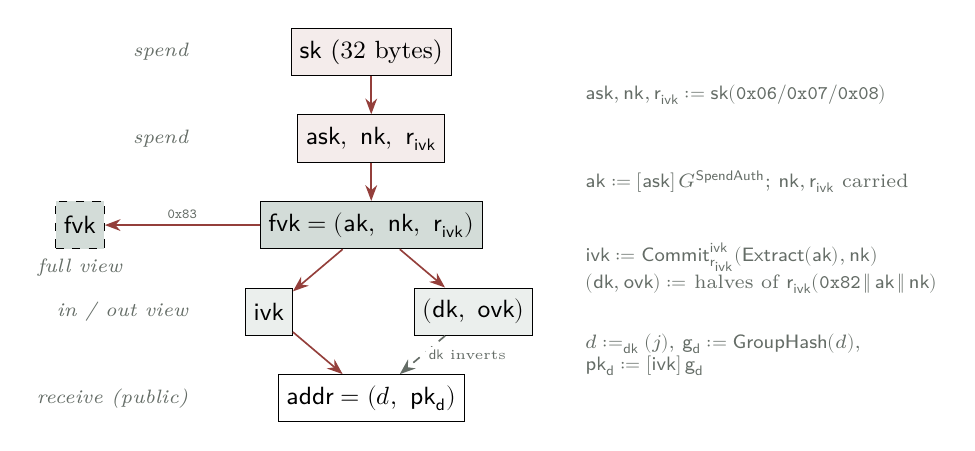
\begin{tikzpicture}[font=\small, x=1cm, y=1cm,
  k/.style={draw, inner sep=3pt, minimum height=6mm,
            anchor=center, fill=arb!10},
  kspend/.style={k, fill=arbred!10},
  kfull/.style={k, fill=arb!22},
  kpub/.style={k, fill=white},
  kint/.style={k, dashed, fill=arb!22},
  tier/.style={font=\scriptsize\itshape, text=arbdim, anchor=east},
  op/.style={font=\scriptsize, text=arbdim, anchor=west, align=left},
  elab/.style={font=\tiny, text=arbdim, inner sep=1pt, fill=white},
  ow/.style={-{Stealth}, thick, arbred},
  inv/.style={-{Stealth}, thick, arbdim, dashed}]
\node[kspend] (sk)    at (0,0)       {$\mathsf{sk}$ (32 bytes)};
\node[kspend] (mid)   at (0,-1.1)    {$\asksym,\ \nksym,\ \rivk$};
\node[kfull]  (fvk)   at (0,-2.2)    {$\fvk = (\aksym,\ \nksym,\ \rivk)$};
\node[kint]   (int)   at (-3.7,-2.2) {$\Dint{\fvk}$};
\node[k]      (ivk)   at (-1.3,-3.3) {$\ivk$};
\node[k]      (dkovk) at (1.3,-3.3)  {$(\dk,\ \ovk)$};
\node[kpub]   (addr)  at (0,-4.4)    {$\mathsf{addr} = (d,\ \pkd)$};
\draw[ow] (sk)  -- (mid);
\draw[ow] (mid) -- (fvk);
\draw[ow] (fvk) -- (ivk);
\draw[ow] (fvk) -- (dkovk);
\draw[ow] (fvk) -- node[elab, above=1pt]{$\mathtt{0x83}$} (int);
\draw[ow] (ivk) -- (addr);
\draw[inv] (dkovk) -- node[elab, right=1pt]{$\dk$ inverts} (addr);
\node[op] at (2.6,-0.55)
  {$\asksym, \nksym, \rivk := \Dprf{\mathsf{sk}}
   (\mathtt{0x06} / \mathtt{0x07} / \mathtt{0x08})$};
\node[op] at (2.6,-1.65)
  {$\aksym := [\asksym]\,G^{\mathsf{SpendAuth}}$; $\nksym, \rivk$ carried};
\node[op] at (2.6,-2.75)
  {$\ivk := \CommitIvk_{\rivk}(\Extract(\aksym), \nksym)$\\
   $(\dk, \ovk) :=$ halves of
   $\Dprf{\rivk}(\mathtt{0x82}\,\|\,\aksym\,\|\,\nksym)$};
\node[op] at (2.6,-3.85)
  {$d := \Dff_{\dk}(j)$, $\gd := \GroupHash(d)$,\\
   $\pkd := [\ivk]\,\gd$};
\node[tier] at (-2.2,0)    {spend};
\node[tier] at (-2.2,-1.1) {spend};
\node[tier, anchor=north] at (int.south) {full view};
\node[tier] at (-2.2,-3.3) {in / out view};
\node[tier] at (-2.2,-4.4) {receive (public)};
\end{tikzpicture}}

\divider{Part D}{Keys and addresses}

% d_keys.py: seed 32..252 bytes, >= 256 bits entropy; sk 32 bytes = 256 bits
% d_keys.py: hardened offset 2^31 = 2147483648; purpose 32' = 0x80000020
%   (shielded), 44' (transparent); coin type 133; accounts 0..2147483647
% d_keys.py: PRFexpand leads: spend 0x06/0x07/0x08, dk|ovk 0x82, internal
%   0x83, CKD 0x81; path levels below master: 3 (all hardened)
% d_keys.py: transparent path: 5 levels below master, 2 non-hardened;
%   Orchard path: 3 levels, all hardened
\begin{frame}{BIP-32 becomes ZIP-32: one seed, two trees}
\[
(\mathsf{sk}_i, c_i) := \text{halves of }
\Dprf{c_{\mathrm{par}}}\bigl(\mathtt{0x81}\,\|\,
\mathsf{sk}_{\mathrm{par}}\,\|\,i\bigr),
\qquad i \ge 2^{31}
\]
\begin{itemize}
  \item One seed (32--252 bytes, at least 256 bits of entropy) roots both
    trees, so one backup recovers every key. Transparent keys keep
    BIP-44: $m/44'/133'/\mathit{account}'/\mathit{change}/\mathit{index}$,
    the two lowest levels non-hardened, an xpub at the account.
  \item Orchard keys stop at
    $m_{\mathsf{Orchard}}/32'/133'/\mathit{account}'$: hardened only,
    every level by the formula above, the chain code discarded at the
    account. The xpub mode --- a public key deriving child public keys ---
    is undefined, so no Orchard extended full viewing key exists.
  \item No change level. BIP-44's change branch separates addresses on a
    public graph; a shielded change output is indistinguishable on chain
    from any other output, so a change subtree would separate nothing.
\end{itemize}
\src{\emph{Wallet Guide}, ``Wallet seeds''; ``Hardened-only derivation'';
``The standard account path''; ZIP-32, ``Key path levels''}
\end{frame}

% d_keys.py: PRFexpand leads: spend 0x06/0x07/0x08, dk|ovk 0x82, internal
%   0x83, CKD 0x81; path levels below master: 3 (all hardened)
% ep_actions.py: amounts: in 200000000 -> Bob 150000000, change 49990000
%   zatoshi (0.4999 ZEC)
\begin{frame}{Two scopes per account: external and internal}
\[
\Dint{\rivk} := \mathrm{ToScalar}\bigl(\Dprf{\rivk}(\mathtt{0x83}\,\|\,
\aksym\,\|\,\nksym)\bigr), \qquad
\Dint{\fvk} := (\aksym,\ \nksym,\ \Dint{\rivk})
\]
\begin{itemize}
  \item Only \rivk{} changes ($\mathrm{ToScalar}$ reduces the $512$-bit
    output modulo the Pallas scalar-field order). The same \asksym{} spends
    and the same \nksym{} nullifies in both scopes; \ivk, \dk, \ovk{} are
    re-derived, so an internal address does not decrypt under the external
    \ivk.
  \item The internal key $\Dint{\fvk}$ follows from \fvk: a full viewing
    key sees both scopes; an external $(\dk, \ivk)$ --- a payment
    processor --- sees the external scope only, never the change: neither
    the internal scope nor any \ovk{} follows from it.
\end{itemize}
\src{\emph{Wallet Guide}, ``Internal keys: change and auto-shielding'';
ZIP-32, ``Orchard internal key derivation''; ZIP-316, ``Deriving Internal
Keys''}
\end{frame}

% ep_actions.py: amounts: in 200000000 -> Bob 150000000, change 49990000
%   zatoshi (0.4999 ZEC)
\begin{frame}{The internal scope: change and auto-shielding}
\begin{itemize}
  \item What BIP-44 puts in the path sits here in the key: internal
    addresses take change and auto-shielded funds. \emph{Shielding} is
    moving transparent funds into the pool; wallets do it automatically,
    to an internal address.
  \item The deployed wallet library (librustzcash) sends change to the
    internal address at index $0$: Alice's $0.4999$ ZEC goes there.
\end{itemize}
\src{\emph{Wallet Guide}, ``Internal keys: change and auto-shielding'';
\emph{Ironwood Guide}, ``The doors: shielding, coinbase, migration''}
\end{frame}

% d_keys.py: sk 32 bytes; PRFexpand leads: spend 0x06/0x07/0x08, dk|ovk
%   0x82, internal 0x83
% d_keys.py: PRFexpand output 512 bits = 64 bytes; dk = first 32 bytes,
%   ovk = last 32 bytes
\begin{frame}{The ladder: one secret, graded capabilities}
\centering
\LadderFig
\par\smallskip
\begin{flushleft}\small
Red arrows are one-way: a rung is handed down without the powers above
it. BIP-32 has two rungs, xprv and xpub, and the public ledger supplies
the rest; here every rung between is a separate secret, and $(\dk, \ovk)$
come from \fvk{} by a PRF, not from \ivk. The circuit re-walks
$\fvk \to \ivk \to \pkd$ (A7) with \gd{} as a witness: the diversifier
step never enters it.
\end{flushleft}
\src{\emph{Ironwood Guide}, ``The capability ladder''; ``Viewing keys'';
``The Action statement, formally''; protocol specification, ``Orchard Key
Components''}
\end{frame}

% d_keys.py: PRFexpand leads: spend 0x06/0x07/0x08, dk|ovk 0x82, internal
%   0x83
\begin{frame}{What holds the rungs apart}
\begin{center}\small
\begin{tabular}{@{}lll@{}}
\toprule
step & operation & why it is one-way \\
\midrule
$\mathsf{sk} \to (\asksym, \nksym, \rivk)$
  & $\Dprf{\mathsf{sk}}(\mathtt{0x06}/\mathtt{0x07}/\mathtt{0x08})$
  & PRF (BLAKE2b) \\
$\asksym \to \aksym$
  & $[\asksym]\,G^{\mathsf{SpendAuth}}$
  & discrete log on Pallas \\
$\fvk \to \ivk$
  & $\CommitIvk_{\rivk}(\Extract(\aksym), \nksym)$
  & hiding under \rivk \\
$\fvk \to (\dk, \ovk)$
  & halves of $\Dprf{\rivk}(\mathtt{0x82}\,\|\,\aksym\,\|\,\nksym)$
  & PRF \\
$\fvk \to \Dint{\fvk}$
  & $\Dprf{\rivk}(\mathtt{0x83}\,\|\,\aksym\,\|\,\nksym)$
  & PRF \\
$\ivk \to \pkd$
  & $[\ivk]\,\gd$
  & discrete log on Pallas \\
$j \to d$
  & $\Dff_{\dk}(j)$
  & \emph{not} one-way: \dk{} inverts it \\
\bottomrule
\end{tabular}
\end{center}
\begin{itemize}
  \item The scalar \ivk{} is a commitment, not a hash, because it must bind
    \emph{and} hide $(\aksym, \nksym)$: an \ivk{} holder learns neither.
    Since \rivk{} also keys the $\mathtt{0x82}$ PRF, hiding rests on a
    joint assumption once \dk{} or \ovk{} is exposed.
  \item Why a separate \nksym: spent status can be delegated without
    spend authority --- the viewing key holds \nksym, never \asksym.
\end{itemize}
\src{\emph{Ironwood Guide}, ``The capability ladder''; \emph{Wallet Guide},
``Diversified addresses''; protocol specification, ``Orchard Key
Components''}
\end{frame}

\begin{frame}{Graded capabilities: spend, full view, spent status}
\begin{center}\small
\begin{tabular}{@{}llp{42mm}p{34mm}@{}}
\toprule
capability & holds & can & cannot \\
\midrule
spend & \asksym{} (from $\mathsf{sk}$)
  & authorise spends, both scopes & --- \\
full view & $\fvk = (\aksym, \nksym, \rivk)$
  & everything below, both scopes; every address and its index
  & spend: \asksym{} is a discrete log away \\
spent status & \nksym{} (inside \fvk)
  & the nullifier of a note it holds
  & spend; find notes (needs \ivk) \\
\bottomrule
\end{tabular}
\end{center}
\begin{itemize}
  \item Bitcoin keeps only the spend row secret (xprv); full view and
    spent status are what its public ledger shows to everyone.
\end{itemize}
\src{\emph{Ironwood Guide}, ``The capability ladder''; \emph{Wallet Guide},
``From the account key to addresses: the layer already built''}
\end{frame}

% d_keys.py: diversifier 88 bits; addresses per account per scope 2^88
\begin{frame}{Graded capabilities: incoming, outgoing, receive}
\begin{center}\small
\begin{tabular}{@{}llp{50mm}p{40mm}@{}}
\toprule
capability & holds & can & cannot \\
\midrule
incoming view & $(\dk, \ivk)$
  & detect and decrypt incoming; derive all $2^{88}$ addresses and
    invert them to indices
  & nullifiers, so spent status; outgoing; the internal scope \\
outgoing view & \ovk
  & open $C_{\mathrm{out}}$ of what this account and scope sent (a sender
    may set $\ovk = \bot$: then no \ovk{} opens it)
  & incoming; the internal \ovk \\
receive & $(d, \pkd)$
  & be paid & anything else --- the only public item \\
\bottomrule
\end{tabular}
\end{center}
\begin{itemize}
  \item Every row but the last is a distinct secret; Bitcoin's ledger
    collapses everything between xprv and the address into what anyone can
    read.
\end{itemize}
\src{\emph{Ironwood Guide}, ``The capability ladder''; ``The outgoing
ciphertext''; \emph{Wallet Guide}, ``Raw encodings''; ZIP-316, ``Deriving
Internal Keys''}
\end{frame}

\begin{frame}{Viewing keys: xpub is the bridge, not the analogue}
\begin{itemize}
  \item An xpub is a watch-only wallet: it enumerates the addresses, and
    the public ledger supplies incoming, outgoing and spent status ---
    to anyone, xpub or not.
  \item The pair $(\dk, \ivk)$ is the watch-only wallet for incoming: it
    enumerates the addresses \emph{and} decrypts. Three differences:
  \begin{enumerate}
    \item Bitcoin shows everything regardless; here nothing is visible
      without the key --- the outputs are ciphertext.
    \item Spent status is a second secret: \nksym{} computes the
      nullifiers that the chain's set is matched against.
    \item Outgoing is a third: \ovk{} opens $C_{\mathrm{out}}$. The xpub
      gets both free only because Bitcoin's ledger is public.
  \end{enumerate}
  \item ``Viewing'' names a capability, not publicity: every viewing key
    is secret material disclosed deliberately --- to an auditor, a
    processor --- and validation needs none of them.
\end{itemize}
\src{\emph{Ironwood Guide}, ``The capability ladder''; ``What a node
verifies, without ever observing the note''; \emph{Wallet Guide},
``Unified viewing keys''}
\end{frame}

% d_keys.py: diversifier 88 bits; addresses per account per scope
%   2^88 = 309485009821345068724781056 ~ 3.1e+26; random draws collide near
%   2^44 = 17592186044416
% d_keys.py: raw receiver 11 + 32 = 43 bytes
\begin{frame}{Diversified addresses: one key, $2^{88}$ addresses}
\begin{gather*}
d := \Dff_{\dk}(j), \qquad
\gd := \Dgh, \\
\pkd := [\ivk]\,\gd, \qquad \mathsf{addr} := (d,\ \pkd)
\end{gather*}
\begin{itemize}
  \item Every index $j$ of the $2^{88} \approx 3.1 \times 10^{26}$ works:
    $\GroupHash$ is total (a fixed fallback covers the identity), so no
    rejection loop. A raw receiver is $11 + 32 = 43$ bytes; all of them
    are spent by one \asksym{} and found by one \ivk, at no extra scanning
    cost.
  \item A keyed permutation, not a counter and not a hash: consecutive
    indices scatter over $\{0,1\}^{88}$, never collide (random 88-bit
    draws would, near $2^{44}$), and \dk{} inverts the map, so the wallet
    stores nothing per address.
  \item Wallet-side only, never in the circuit --- which is why AES is
    fine here.
\end{itemize}
\src{\emph{Ironwood Guide}, ``Diversified addresses''; \emph{Wallet Guide},
``Diversified addresses''; ``Raw encodings''; \emph{Crypto Guide},
``Format-preserving encryption and FF1''; ZIP-32, ``Orchard key path''}
\end{frame}

% d_keys.py: diversifier 88 bits; addresses per account per scope 2^88
\begin{frame}{Unlinkable, even to the payer}
\[
(d, \pkd) \quad\text{and}\quad (d', \pkd'):
\quad \pkd = [\ivk]\,\gd,\ \ \pkd' = [\ivk]\,\gd'
\quad\text{--- same \ivk?}
\]
\begin{itemize}
  \item Deciding it is a DDH problem on Pallas with $\GroupHash$ as a
    random oracle: given two addresses of different owners and a third
    derived from one of them, no one can tell which. Alice, who paid one
    of Bob's addresses, learns nothing about the other.
  \item Only the holder of $(\dk, \ivk)$ can check --- by re-deriving the
    address at the decrypted index under that \ivk.
  \item One rule for implementers: never offer a chosen-diversifier
    oracle (an address for an attacker's $d$ under your \ivk): it breaks
    unlinkability for every address of that \ivk.
  \item Under one xpub, addresses link on the public graph once spent
    together (Part A); a leaked xpub links all beneath it, spent or not.
    Here an address reveals only itself.
\end{itemize}
\src{\emph{Wallet Guide}, ``Diversified addresses''; \emph{Ironwood Guide},
``Diversified addresses''; protocol specification,
``$\mathsf{DiversifyHash}^{\mathsf{Sapling}}$ and
$\mathsf{DiversifyHash}^{\mathsf{Orchard}}$ Hash Functions''}
\end{frame}

% d_keys.py: typecodes: 0x00 P2PKH, 0x01 P2SH, 0x02 Sapling, 0x03 Orchard;
%   priority = descending typecode
\begin{frame}{Unified addresses (ZIP-316): one string, several receivers}
\begin{itemize}
  \item One string carries at most one receiver per type --- transparent
    P2PKH or P2SH ($\mathtt{0x00}$/$\mathtt{0x01}$), Sapling
    ($\mathtt{0x02}$), Orchard ($\mathtt{0x03}$) --- with at least one
    shielded. Items are encoded in ascending typecode, passed through
    F4Jumble --- an unkeyed four-round Feistel permutation of the whole
    payload, HRP included --- then Bech32m: a substituted receiver
    changes the whole string, not one region of it.
  \item What a sender does: use the most preferred receiver it supports
    --- Orchard over Sapling over transparent; a wallet may refuse a type,
    never reorder.
  \item Which pool: an Orchard receiver names the protocol, not a pool,
    and all new value enters the Ironwood pool, so a payment to it lands
    in the Ironwood tree; the receiver has no string form of its own.
  \item The same container with viewing-key items is a unified full or
    incoming viewing key.
  \item Bitcoin: one address encodes one script type; here one address
    lets the sender's wallet choose the pool.
\end{itemize}
\src{\emph{Wallet Guide}, ``Unified addresses''; ``String encoding:
F4Jumble and Bech32m''; ``Unified viewing keys''; \emph{Ironwood Guide},
``One ladder, both pools''; ZIP-316, ``Encoding of Unified Addresses''}
\end{frame}

% d_keys.py: Bob receives 1.5 ZEC = 150000000 zatoshi; Ironwood lead byte
%   0x03; raw receiver 11 + 32 = 43 bytes
% ep_actions.py: amounts: in 200000000 -> Bob 150000000, change 49990000
%   zatoshi (0.4999 ZEC)
\begin{frame}{Bob's address in the example}
Bob hands Alice a unified address; her wallet takes its Orchard receiver
$\mathsf{addr}_B = (d_B, \pkd)$, 43 bytes, and derives
\begin{gather*}
\gd := \GroupHash^{\Pallas}(\mathtt{z.cash:Orchard\text{-}gd},\ d_B),
\qquad \epk := [\esk]\,\gd, \\
\mathbf{n} := (\mathsf{addr}_B,\ 1.5\ \text{ZEC},\ \rho,\ \psi,\ \rcm).
\end{gather*}
\begin{itemize}
  \item That is all it learns: no \ivk, \nksym, \aksym, no index $j$, no
    link to Bob's other addresses. On chain the address appears only
    blinded: inside \cmsym, inside $C_{\mathrm{enc}}$, and as \epk{} under
    a fresh \esk.
  \item Minted in the Ironwood tree, lead byte $\mathtt{0x03}$; Bob's one
    \ivk{} trial-decrypts both pools.
  \item Her change, $0.4999$ ZEC, goes to her internal address at index
    $0$: no address of hers appears either.
  \item Bitcoin displays the script beside the amount; here neither
    appears in the clear.
\end{itemize}
\src{\emph{Ironwood Guide}, ``Sender: one-shot Diffie--Hellman and the
AEAD''; ``The note and its commitment''; ``One ladder, both pools'';
\emph{Wallet Guide}, ``Unified addresses''; ``Internal keys: change and
auto-shielding''}
\end{frame}

% d_keys.py: PRFexpand leads: spend 0x06/0x07/0x08, dk|ovk 0x82, internal
%   0x83
\begin{frame}{Checkpoint}
\begin{center}
\Large Which key does an accountant need to audit a company's incoming
\emph{and} outgoing shielded payments --- and what can they not do with
it?
\end{center}
\pause
\medskip
\begin{itemize}
  \item One unified full viewing key per account. Inside it, \fvk{} yields
    \ivk{} (incoming), \nksym{} (which of those notes are spent) and
    \ovk{} (outgoing) --- for the external scope and, through the
    $\mathtt{0x83}$ step, the internal one, so change is covered too.
  \item Not spend: \asksym{} is a discrete logarithm away from \aksym.
    Not wander into a sibling account: only hardened derivation exists,
    and no Orchard extended full viewing key.
  \item Not read what was sent under some other \ovk, or under none: the
    sender may set $\ovk = \bot$, and then no \ovk{} opens
    $C_{\mathrm{out}}$. Nor anything received by an account they were not
    given.
\end{itemize}
\src{\emph{Ironwood Guide}, ``The capability ladder''; ``The outgoing
ciphertext''; \emph{Wallet Guide}, ``From the account key to addresses:
the layer already built''; ``Internal keys: change and auto-shielding'';
``Unified viewing keys''}
\end{frame}

%% ---- 05-statement.tex
%% ---- Part E --- The Action statement (E1--E11, then the break)
\newcommand{\Ecv}{\ensuremath{\cvsym^{\mathsf{net}}}}
\newcommand{\Enf}{\ensuremath{\nfsym_{\mathrm{old}}}}
\newcommand{\Eanc}{\ensuremath{\mathsf{anchor}}}
\newcommand{\Eold}[1]{\ensuremath{#1_{\mathrm{old}}}}
\newcommand{\Enew}[1]{\ensuremath{#1_{\mathrm{new}}}}
\newcommand{\Ecenc}{\ensuremath{C_{\mathrm{enc}}}}
\newcommand{\Ecout}{\ensuremath{C_{\mathrm{out}}}}
\newcommand{\Eflag}[1]{\ensuremath{\mathsf{#1}}}
\newcommand{\EPoseidon}{\ensuremath{\mathsf{Poseidon}}}
\newcommand{\Egsa}{\ensuremath{G^{\mathsf{SpendAuth}}}}
\newcommand{\Egnf}{\ensuremath{G^{\mathsf{nf}}}}
% \ActionBox[field]: one Action (witness inside, public fields on the rim)
% inside its bundle; field in {none, anchor, nf, cv, rk, cmx, proof} is
% drawn highlighted. Defined here once; later fragments reuse it.
\newcommand{\ActionBox}[1][none]{%
  \tikzset{hlnone/.style={}, hlanchor/.style={}, hlnf/.style={},
    hlcv/.style={}, hlrk/.style={}, hlcmx/.style={}, hlproof/.style={},
    hl#1/.style={draw=arbred, very thick, fill=arbred!15}}%
  \begin{tikzpicture}[font=\scriptsize, x=1cm, y=1cm,
    ebox/.style={draw=black!60, fill=white,
      inner sep=2.5pt, align=center},
    elab/.style={inner sep=2pt, text=black!60}]
  % the bundle; a second Action behind the first
  \draw[draw=black!50, dashed]
    (-2.45,-2.45) rectangle (4.75,2.5);
  \node[elab, anchor=north west, text=black!70, font=\scriptsize\bfseries]
    at (-2.45,2.5) {bundle};
  \draw[draw=arb!40] (-2.0,-2.1) rectangle (2.4,2.1);
  \node[elab, anchor=south east, text=arb!60] at (2.4,2.1) {$\times\,n$};
  \node[draw=arb, thick, fill=white,
    minimum width=4.4cm, minimum height=3.9cm] (act) at (0,0) {};
  \node[anchor=north west, font=\scriptsize\bfseries, text=arb,
    inner sep=2pt] at (act.north west) {Action};
  \node[draw=arb!60, fill=arb!8, inner sep=3pt,
    align=center, anchor=north, text width=3.8cm] (wit) at (0,1.62)
    {\textbf{witness} --- never published\\
     old note, new note\\
     Merkle path $+$ position\\
     $\aksym, \nksym, \rivk, \ivk$; $\alpha$, $\rcv$};
  \node[elab, anchor=west] at (-2.15,-0.12) {public, per Action};
  \node[ebox, hlcv, anchor=west] (cv) at (-2.05,-0.58) {$\Ecv$};
  \node[ebox, hlnf, right=1.2mm of cv] (nf) {$\Enf$};
  \node[ebox, hlrk, right=1.2mm of nf] (rk) {$\rksym$};
  \node[ebox, hlcmx, right=1.2mm of rk] (cmx) {$\cmx$};
  \node[ebox, draw=black!40, dashed] (ct) at (0,-1.15)
    {$\epk,\ \Ecenc,\ \Ecout$};
  \node[elab, align=center, font=\tiny, text=black!60] at (0,-1.66)
    {delivery ciphertexts --- no in-circuit check;\\
     opened only with $\ivk$/$\ovk$ (\emph{Delivery})};
  % bundle-level fields
  \node[ebox, hlanchor, anchor=west] (anc) at (2.45,1.65) {$\Eanc$};
  \node[ebox, anchor=west] (flg) at (2.45,1.0) {flags};
  \node[ebox, anchor=west] (vb)  at (2.45,0.35) {$v_{\mathrm{balance}}$};
  \node[ebox, hlproof, anchor=west] (prf) at (2.45,-0.3) {proof};
  \node[ebox, anchor=west] (sas) at (2.45,-0.95) {SpendAuthSigs};
  \node[ebox, anchor=west] (bsg) at (2.45,-1.6) {binding sig};
  \end{tikzpicture}}

\divider{Part E}{The Action statement}

% compute/e_action.py:
%   OrchardAction bytes: 32 + 32 + 32 + 32 + 32 + 580 + 80 = 820
%   ciphertext share: 660 of 820
%   Alice: s=1 spend, o=2 outputs (Bob, change) -> n_act = 2;
%     dummy spends 1, dummy outputs 0
%   named public inputs: 8; instance elements: 1+2+1+2+1+1+1+1 = 10;
%     clauses A1..A10 = 10
% compute/e_clauses.py:
%   public per Action: 4 proof-bound (cv, nf, rk, cmx) + 3 delivery
%     (epk, C_enc, C_out); per bundle: anchor, flags, valueBalance, proof,
%     SpendAuthSigs, binding sig
\begin{frame}{Anatomy of an Action}
\begin{columns}[T]
\begin{column}{0.52\textwidth}
\centering\ActionBox
\end{column}
\begin{column}{0.46\textwidth}
\begin{itemize}\small
  \item One Action spends one old note and creates one new one; the
    shape is fixed, so an Action never shows which it ``really'' is.
  \item Inside: the witness --- both notes, the path, the keys,
    $\alpha$, $\rcv$ --- never published.
  \item On the rim, per Action: $\Ecv$, $\Enf$, $\rksym$, $\cmx$ ---
    the four fields the proof binds.
  \item Dashed: $\epk$, $\Ecenc$, $\Ecout$ --- delivery ciphertexts,
    read by no clause; only $\ivk$ or $\ovk$ opens them
    (\emph{Delivery and light clients}).
\end{itemize}
\end{column}
\end{columns}
\smallskip
\small A Bitcoin input names its coin and shows its script; a Bitcoin
output shows its amount and its script. Here every field is a
commitment, a serial number, a disguised key, or a ciphertext.
\src{\emph{Ironwood Guide}, ``One Action, one payment: the walkthrough'';
``The outgoing ciphertext''; ``The Action statement, formally''}
\end{frame}

% compute/e_action.py:
%   OrchardAction bytes: 32 + 32 + 32 + 32 + 32 + 580 + 80 = 820
%   ciphertext share: 660 of 820
% compute/ep_actions.py:
%   Actions: 2 (requested spends 1, outputs 2, padded to the floor of 2)
%   bytes: Actions 820 * 2 = 1640; proof 2720 + 2272 * 2 = 7264;
%     SpendAuthSigs 64 * 2 = 128; binding sig 64; signatures 128 + 64 = 192
\begin{frame}{The bundle around it}
\begin{center}\small
\begin{tabular}{@{}lp{5.4cm}p{6.2cm}@{}}
\toprule
per bundle & once & role \\
\midrule
$\Eanc$ & one root, shared by every Action & the tree the spends
  prove membership in \\
flags & $\Eflag{enableSpends}$, $\Eflag{enableOutputs}$,\newline
  $\Eflag{enableCrossAddress}$ & consensus gates (A8--A10) \\
$v_{\mathrm{balance}}$ & signed, cleartext & net value leaving the
  pool \\
proof & one aggregate Halo 2 proof & covers all $n$ Actions at once \\
binding sig & one signature & proves the values balance \\
\addlinespace
per Action & SpendAuthSig under $\rksym$ & the owner authorised this
  spend \\
\bottomrule
\end{tabular}
\end{center}
\medskip
\small
\begin{itemize}
  \item Each Action is $820$ public bytes, $660$ of them ciphertext;
    Alice's bundle carries two Actions and one $7264$-byte proof.
  \item The node checks the proof, the anchor, the nullifier set, and
    the two signatures --- and never sees a note. Both signatures and
    $v_{\mathrm{balance}}$ return in \emph{Balance and authority}.
\end{itemize}
\src{\emph{Ironwood Guide}, ``What a node verifies, without ever
observing the note''; ``The v6 transaction and the Ironwood component''}
\end{frame}

% compute/e_action.py:
%   Alice: s=1 spend, o=2 outputs (Bob, change) -> n_act = 2;
%     dummy spends 1, dummy outputs 0
% compute/ep_actions.py:
%   Actions: 2 (requested spends 1, outputs 2, padded to the floor of 2)
%   fee = 5000 * max(2, 2) = 10000 zatoshi
\begin{frame}{Why a spend and an output are fused}
\[
n_{\mathrm{act}}(s, o) = \max\bigl(\max(s, o),\, 2\bigr)
\qquad\text{Alice: } s = 1,\ o = 2 \;\Rightarrow\; n_{\mathrm{act}} = 2
\]
\begin{itemize}
  \item \textbf{Uniformity.} Every Action looks like every other: one
    spend slot, one output slot, whatever the payment needed.
  \item \textbf{Padding.} The spend list and the output list are each
    extended to $n_{\mathrm{act}}$; the floor is two. Alice's one spend
    and two outputs (Bob, change) pad with one dummy spend.
  \item \textbf{Scope.} This count, and the shuffle on the next slide,
    are the Ironwood component's (cross-address enabled). A sealed
    Orchard-pool bundle pads to $s + o$ and pairs each spend with an
    output to the spent note's own receiver.
\end{itemize}
\medskip
\small A Bitcoin transaction shows its true input and output counts;
here the count is $n_{\mathrm{act}}$, and the fee is computed from that
public count (\emph{The transaction and the turnstile}).
\src{\emph{Wallet Guide}, ``Padding, dummies, and shuffling''; \emph{Ironwood
Guide}, ``Spending under the restriction''}
\end{frame}

\begin{frame}{Dummies and the shuffle}
\begin{itemize}
  \item \textbf{Dummies.} A slot with nothing real in it holds a
    \emph{dummy}. A dummy spend is a zero-value note under a fresh
    random spending key, its $\rho$ the $\Extract$ of a random Pallas
    point; it still publishes a nullifier. A dummy output is a
    zero-value note to a fresh random address, its $\rho := \Enf$ like
    any output's.
  \item \textbf{Shuffling.} Spends and outputs are shuffled
    \emph{independently}, then zipped: which spend shares an Action
    with which output is random.
  \item Alice's bundle: her $2$ ZEC note and a dummy on the spend side,
    Bob's note and her change on the output side; which pair forms which
    Action is the shuffle's choice.
\end{itemize}
\medskip
\small A Bitcoin input is an input and an output is an output; here a
dummy spend looks exactly like a real one and, like a real one,
publishes a nullifier the pool records.
\src{\emph{Wallet Guide}, ``Padding, dummies, and shuffling''; \emph{Ironwood
Guide}, ``The nullifier, and the loop back to minting''; protocol
specification, ``Dummy Notes (Orchard)''}
\end{frame}

% compute/e_action.py:
%   named public inputs: 8; instance elements: 1+2+1+2+1+1+1+1 = 10;
%     clauses A1..A10 = 10
\begin{frame}{The statement, in the validator's language}
\emph{``Some leaf under this anchor is a note I own; this is its serial
number; this commitment hides its value change; this signing key is a
fresh disguise of the owner's --- and I have shown you neither the leaf,
the note, nor the owner's key.''}
\medskip
\begin{itemize}
  \item \textbf{Public inputs:} $\Eanc$, $\Ecv$, $\Enf$, $\rksym$,
    $\cmx$ and the three flags --- eight names, ten field elements
    (the two Pallas points enter by their coordinates). Here $\Ecv$ and
    $\Enf$ are the data model's $\cvsym$ and $\nfsym$, marked \emph{net}
    (this Action's value change) and \emph{old} (the note spent).
  \item \textbf{Witness:} both notes, the path and position, $\aksym$,
    $\nksym$, $\rivk$, $\ivk$, $\alpha$, $\rcv$.
  \item \textbf{Relation:} ten clauses, A1--A10, over those inputs.
    The node's verifying key fixes exactly these ten, selected by
    branch; a proof of nine is a proof for a different circuit, and
    it fails.
\end{itemize}
\medskip
\small Bitcoin's validator runs \emph{your} script. This validator runs
one verifier keyed to one fixed circuit; the transaction supplies
inputs, never logic.
\src{\emph{Ironwood Guide}, ``The Action statement, formally''; ``One
circuit, one verifying key''; protocol specification, ``Action Statement
(Orchard)''}
\end{frame}

% compute/e_action.py:
%   named public inputs: 8; instance elements: 1+2+1+2+1+1+1+1 = 10;
%     clauses A1..A10 = 10
% compute/a_checks.py:
%   (1) coin exists      Bitcoin: UTXO lookup   ... (A3)
%   (2) authorised       Bitcoin: script + signature ... (A6/A7)
%   (3) not spent twice  Bitcoin: UTXO deleted  ... (A5)
%   (4) conserved        Bitcoin: sum(in) >= sum(out) ... (A4)
% compute/e_clauses.py:
%   spine clauses: 7 (A1-A7); consensus gates: 3 (A8-A10)
\begin{frame}{The ten clauses, ordered by the four checks}
\begin{center}\small
\begin{tabular}{@{}llp{7.4cm}@{}}
\toprule
Bitcoin's check & clause & what the proof establishes \\
\midrule
coin exists (UTXO lookup) & A3 & a Merkle path from $\Eold{\cmsym}$ to
  the anchor \\
not spent twice (entry deleted) & A5 & $\Enf$ is this note's serial,
  keyed by $\nksym$ \\
conserved ($\sum\mathrm{in} \ge \sum\mathrm{out}$) & A4 & $\Ecv$ hides
  $\Eold{v} - \Enew{v}$, both below $2^{64}$ \\
authorised (script $+$ signature) & A6, A7 & $\rksym$ disguises
  $\aksym$; $\aksym, \nksym$ sit behind the address \\
\addlinespace
well-formed & A1, A2 & both commitments open to notes;
  $\Enew{\rho} = \Enf$ \\
gated & A8, A9 & spends and outputs switched on by the flags \\
sealed & A10 & cross-address transfers switched off, or not \\
\bottomrule
\end{tabular}
\end{center}
\medskip
\small Four of Bitcoin's checks become seven clauses; three more are
consensus gates the flags drive. The remaining check --- ``has this
serial been seen?'' --- is global history and stays with the node.
\src{\emph{Ironwood Guide}, ``The Action statement, formally''; ``The four
requirements on a shielded payment''; ``What a node verifies, without
ever observing the note''}
\end{frame}

% compute/e_clauses.py:
%   Action 1: v_old 200000000 v_new 150000000 net +50000000 zatoshi
%     (+0.5 ZEC); A3 checked (v_old != 0); A8 product 0, A9 product 0;
%     A10 delta = 0, products 4 * 0 = 0
%   Action 2 (dummy spend): v_old 0 v_new 49990000 net -49990000 zatoshi
%     (-0.4999 ZEC); A3 gated off (v_old = 0); A8 product 0, A9 product 0;
%     A10 delta = 0, products 4 * 0 = 0
%   sum of nets = +10000 zatoshi = valueBalance = fee
%   clauses: 10; per Action A3 gated for 1 of 2; A2 chains rho_new :=
%     nf_old in both
% compute/e_tree.py:
%   depth 32: 2^32 = 4294967296 leaves; path = 32 siblings
\begin{frame}{Alice's two Actions against the ten clauses}
\begin{center}\small
\begin{tabular}{@{}lp{6.1cm}p{6.1cm}@{}}
\toprule
clause & Action 1: $2$ ZEC $\to$ Bob $1.5$ & Action 2: dummy $\to$
  change $0.4999$ \\
\midrule
A1 & Alice's $2$ ZEC note opens $\Eold{\cmsym}$ & a zero-value dummy
  opens $\Eold{\cmsym}$ \\
A2 & Bob's note; $\Enew{\rho} := \nfsym$ of Alice's note & change note;
  $\Enew{\rho} := \nfsym$ of the dummy \\
A3 & a $32$-sibling path to the Ironwood anchor & gated off:
  $\Eold{v} = 0$ \\
A4 & $\Ecv$ commits to $+0.5$ ZEC & $\Ecv$ commits to $-0.4999$ ZEC \\
A5 & $\nfsym$ of Alice's note, under her $\nksym$ & $\nfsym$ of the
  dummy, under its random $\nksym$ \\
A6 & $\rksym = \aksym + [\alpha]\,\Egsa$, Alice's $\aksym$ & the same,
  the dummy's $\aksym$ \\
A7 & Alice's $\aksym, \nksym$ sit behind her address & the dummy's
  key, behind its address \\
A8, A9 & both flags set: both products vanish & the same \\
A10 & $\delta = 0$ (Ironwood): nothing constrained & the same \\
\bottomrule
\end{tabular}
\end{center}
\smallskip
\small The two net values sum to $+0.5 - 0.4999 = +0.0001$ ZEC $=
10\,000$ zatoshi: the fee, and the bundle's $v_{\mathrm{balance}}$
(\emph{Balance and authority}).
\src{\emph{Ironwood Guide}, ``The Action statement, formally''; \emph{Wallet
Guide}, ``Padding, dummies, and shuffling''; ``The conventional fee''}
\end{frame}

% compute/e_clauses.py:
%   Action 1: ... net +50000000 zatoshi (+0.5 ZEC)
%   Action 2 (dummy spend): ... net -49990000 zatoshi (-0.4999 ZEC)
%   sum of nets = +10000 zatoshi = valueBalance = fee
%   Ironwood flags (spends, outputs, cross) = (1, 1, 1) -> delta = 0
%   public per Action: cv, nf, rk, cmx + (epk, C_enc, C_out); per bundle:
%     anchor, flags, valueBalance, proof, SpendAuthSigs, binding sig
% compute/ep_actions.py:
%   public per Action: nf, cmx, cv, rk, epk, C_enc, C_out -> 2 nullifiers,
%     2 commitments
\begin{frame}{What Alice's public fields carry}
\begin{center}\small
\begin{tabular}{@{}lp{5.95cm}p{5.95cm}@{}}
\toprule
field & Action 1 & Action 2 \\
\midrule
$\Ecv$ & $+0.5$ ZEC under a fresh $\rcv$ & $-0.4999$ ZEC under a fresh
  $\rcv$ \\
$\Enf$ & Alice's note's serial: the note is retired & the dummy's
  serial, recorded all the same \\
$\rksym$ & a fresh disguise of Alice's $\aksym$ & a fresh disguise of
  the dummy's $\aksym$ \\
$\cmx$ & Bob's $1.5$ ZEC note & Alice's $0.4999$ ZEC change note, at
  her internal address \\
$\epk, \Ecenc$ & to Bob's $\pkd$; opened with his $\ivk$ & to Alice's
  internal $\pkd$; found with $\ivk^{\mathsf{int}}$ \\
$\Ecout$ & under Alice's $\ovk$: she can re-read it & no $\ovk$ for
  change (wallet default):\newline unrecoverable \\
\addlinespace
bundle & \multicolumn{2}{p{12.1cm}@{}}{one Ironwood anchor; flags
  $(1, 1, 1)$; $v_{\mathrm{balance}} = +10\,000$ zatoshi; one proof;
  two SpendAuthSigs; one binding signature} \\
\bottomrule
\end{tabular}
\end{center}
\smallskip
\small Which of the two is ``Action 1'' on the wire is decided by the
shuffle. Two nullifiers, two commitments: the shape of every two-Action
bundle.
\src{\emph{Ironwood Guide}, ``The outgoing ciphertext''; \emph{Wallet
Guide}, ``Padding, dummies, and shuffling''; ``Internal keys: change and
auto-shielding''; ``Executing the proposal''}
\end{frame}

% compute/e_tree.py:
%   depth 32: 2^32 = 4294967296 leaves; path = 32 siblings
\begin{frame}{Coin exists --- A3, the path to the anchor}
\vspace{-4pt}
\begin{center}
Fold $\Extract(\Eold{\cmsym})$ up $32$ witnessed siblings to
$\mathsf{root}$; then
$\ \Eold{v} \cdot (\mathsf{root} - \Eanc) = 0$.
\end{center}
\vspace{-4pt}
\begin{columns}[T]
\begin{column}{0.52\textwidth}
\centering\ActionBox[anchor]
\end{column}
\begin{column}{0.46\textwidth}
\begin{itemize}\small
  \item Witness: the siblings and the position bits. Public: the
    anchor, one per bundle.
  \item Bitcoin looks the coin up in the UTXO set, and so names it.
    This clause says only ``some leaf under this anchor'': the
    candidate set is the Ironwood tree under the anchor.
  \item A zero-value dummy skips the check by arithmetic, not by a
    flag.
\end{itemize}
\smallskip
\alert{Which of the four checks?}\pause\ --- coin exists.
\end{column}
\end{columns}
\src{\emph{Ironwood Guide}, ``The tree, its hash, and its anchors'';
``Anchor choice, reorgs, and the anonymity set''; ``The Action
statement, formally''}
\end{frame}

% compute/e_clauses.py:
%   mental model: 3 lines (A3 membership, A5 serial, A4 balance)
\begin{frame}{No double spend --- A5, the nullifier}
\vspace{-6pt}
\[
\Enf = \Extract\bigl([\,\EPoseidon_{\nksym}(\Eold{\rho}) +
  \Eold{\psi}\,]\,\Egnf + \Eold{\cmsym}\bigr)
\]
\vspace{-10pt}
\begin{columns}[T]
\begin{column}{0.52\textwidth}
\centering\ActionBox[nf]
\end{column}
\begin{column}{0.46\textwidth}
\begin{itemize}\small
  \item Clause A5 binds the published serial to the spent note under
    the witnessed $\nksym$; otherwise a spender could invent a fresh
    serial per spend and the set would never repeat.
  \item ``Seen before?'' is global history: the node checks the set,
    the proof cannot.
  \item Bitcoin deletes the entry; here an unlinkable serial is added.
    The opening's three lines: membership (A3), serial (A5), balance
    (A4, \emph{Balance and authority}).
\end{itemize}
\smallskip
\alert{Which check?}\pause\ --- not spent twice.
\end{column}
\end{columns}
\src{\emph{Ironwood Guide}, ``The nullifier, and the loop back to
minting''; ``What a node verifies, without ever observing the note''}
\end{frame}

\begin{frame}{Authorised --- the linkage problem first}
\begin{gather*}
\ivk = \CommitIvk_{\rivk}\bigl(\Extract(\aksym), \nksym\bigr), \qquad
\pkd = [\ivk]\,\gd \quad\text{for every } d
\end{gather*}
\begin{itemize}
  \item One spend key $\aksym$ per wallet, not per coin: every
    diversified address shares it through $\ivk$ (\emph{Keys and
    addresses}).
  \item The obvious design --- publish $\aksym$ and a signature under
    it --- would stamp every spend the wallet ever makes with one key:
    every note it spends, from every address, linked.
  \item Bitcoin's version of this is address reuse, and it is
    optional. Here it would be structural.
  \item Needed: a key that is fresh for every spend and still proves
    the same secret.
\end{itemize}
\src{\emph{Crypto Guide}, ``Key re-randomisation and unlinkability'';
\emph{Ironwood Guide}, ``Spend authorisation: RedPallas
re-randomisation''}
\end{frame}

\begin{frame}{Authorised --- A6, a disguised key}
\vspace{-6pt}
\[
\rksym = \aksym + [\alpha]\,\Egsa, \qquad \rsk = \asksym + \alpha
\]
\vspace{-10pt}
\begin{columns}[T]
\begin{column}{0.52\textwidth}
\centering\ActionBox[rk]
\end{column}
\begin{column}{0.46\textwidth}
\begin{itemize}\small
  \item Clause A6: the published key is $\aksym$ shifted by a fresh,
    secret $\alpha$. The circuit checks the shift; the node checks a
    signature under $\rksym$ (\emph{Balance and authority}).
  \item Uniform $\alpha$ makes $\rksym$ uniform whatever $\aksym$ is.
  \item Schnorr with a per-spend tweak: a non-hardened BIP-32 child
    whose tweak is uniform and never published.
\end{itemize}
\smallskip
\alert{Which check?}\pause\ --- authorised.
\end{column}
\end{columns}
\src{\emph{Ironwood Guide}, ``Spend authorisation: RedPallas
re-randomisation''; \emph{Crypto Guide}, ``Key re-randomisation and
unlinkability''}
\end{frame}

\begin{frame}{Authorised --- A7, one identity behind the address}
\begin{gather*}
\ivk = \CommitIvk_{\rivk}\bigl(\Extract(\aksym), \nksym\bigr), \qquad
\Eold{\pkd} = [\ivk]\,\Eold{\gd}
\end{gather*}
\begin{itemize}
  \item Clause A6 alone proves a disguise of \emph{some} $\aksym$; A7
    ties that
    $\aksym$, and the $\nksym$ of A5, to the spent note's address by
    the ladder of \emph{Keys and addresses}.
  \item One identity signs (A6), nullifies (A5), and is paid (A7): the
    same secret behind all three, and none of them published.
  \item Authority is split in two: the circuit proves the key is the
    owner's; the signature under $\rksym$ proves the spender holds it
    (\emph{Balance and authority}).
\end{itemize}
\medskip
\small In Bitcoin a P2PKH address \emph{is} the key's hash, so ``this key
matches this coin'' is one hash comparison in the clear. Here the
address is a commitment to the key, and the match is proved.
\src{\emph{Ironwood Guide}, ``The Action statement, formally''; ``Spend
authorisation: RedPallas re-randomisation''}
\end{frame}

\begin{frame}{Well-formed --- A1 and A2, both notes really are notes}
\begin{gather*}
\Eold{\cmsym} = \NoteCommit_{\Eold{\rcm}}(\mathbf{n}_{\mathrm{old}}),
\qquad
\Extract\bigl(\NoteCommit_{\Enew{\rcm}}(\mathbf{n}_{\mathrm{new}})\bigr)
= \cmx, \\
\text{with } \Enew{\rho} := \Enf .
\end{gather*}
\begin{itemize}
  \item Clause A1: the object being spent opens as a note --- address,
    value, $\rho$, $\psi$ --- under the witnessed $\rcm$; the commitment is
    binding, so one leaf cannot be reopened as a second note.
  \item Clause A2: the created note is committed the same way, and the
    chain stores only $\cmx$.
  \item The chain $\Enew{\rho} := \Enf$ is enforced \emph{here}: the new
    note's seed is the serial this Action reveals, so accepted seeds
    are unique within the pool and two notes cannot share a nullifier.
\end{itemize}
\medskip
\small A Bitcoin output is plaintext: well-formed means it parses.
Here the note is hidden, so ``this commitment opens to a note'' must be
proved.
\src{\emph{Ironwood Guide}, ``The note and its commitment''; ``The
nullifier, and the loop back to minting''; ``The Action statement,
formally''}
\end{frame}

% compute/e_range.py:
%   value bound 2^64 = 18446744073709551616;
%   MAX_MONEY = 2100000000000000 zatoshi; MAX_MONEY < 2^64: True
%   Pallas group order: 255 bits, i.e. about 2^254
%   2^16 Actions * 2^64 = 2^80 < 2^254: True
\begin{frame}{Conserved --- A4, the value commitment}
\vspace{-6pt}
\[
\Ecv = [\Eold{v} - \Enew{v}]\,V + [\rcv]\,R, \qquad
\Eold{v}, \Enew{v} \in [0, 2^{64}),\quad \text{sign} \in \{-1, +1\}
\]
\vspace{-10pt}
\begin{columns}[T]
\begin{column}{0.52\textwidth}
\centering\ActionBox[cv]
\end{column}
\begin{column}{0.46\textwidth}
\begin{itemize}\small
  \item Clause A4 commits to this Action's value \emph{change} under a
    fresh trapdoor $\rcv$; the bundle sums these (\emph{Balance and
    authority}).
  \item The range is the point: the sum lives in a group of order about
    $2^{254}$, where a value near the order is a small negative one.
    Unbounded, the books would ``balance'' while minting.
  \item Elements' range proof exists for the same reason; here it lives
    inside the Action proof, with the opening.
\end{itemize}
\smallskip
\alert{Which check?}\pause\ --- conserved.
\end{column}
\end{columns}
\src{\emph{Ironwood Guide}, ``Conservation without disclosure: value
commitments and the binding signature''; ``Balance preservation''}
\end{frame}

% compute/e_clauses.py:
%   Ironwood flags (spends, outputs, cross) = (1, 1, 1) -> delta = 0
%   Action 2 (dummy spend): v_old 0 ...; A8 product 0, A9 product 0
\begin{frame}{Gated --- A8 and A9, the flags}
\begin{gather*}
\Eold{v} \cdot (1 - \Eflag{enableSpends}) = 0, \qquad
\Enew{v} \cdot (1 - \Eflag{enableOutputs}) = 0
\end{gather*}
\begin{itemize}
  \item The flags are bundle-level bits the node supplies as public
    inputs; the circuit only multiplies.
  \item With a flag clear, only a zero value passes: a cleared
    $\Eflag{enableSpends}$ admits dummies and nothing else.
  \item A coinbase must clear $\Eflag{enableSpends}$: its Actions spend
    dummies and create the block's shielded reward. Ordinary bundles
    set both flags, as Alice's does.
\end{itemize}
\medskip
\small Bitcoin's coinbase has one null input by format. Here the same
rule is arithmetic on a hidden value --- the only way to gate what the
node cannot read.
\src{\emph{Ironwood Guide}, ``The Action statement, formally''; ``The
doors: shielding, coinbase, migration''; ``Flags, public inputs, and
circuit parameters''}
\end{frame}

% compute/e_clauses.py:
%   Orchard pool: enableCrossAddress = 0 -> delta = 1; A10 coordinate
%     equalities: 2 points * 2 coordinates = 4
%   Ironwood flags (spends, outputs, cross) = (1, 1, 1) -> delta = 0
%   disableCrossAddress: instance index 9, the tenth of 10 public inputs
% compute/b_seal.py:
%   flags byte: Orchard 0b011 (bit 2 = 0b100 clear), Ironwood 0b111
%     (bit 2 set)
\begin{frame}{Sealed --- A10, the cross-address gate}
\begin{gather*}
\delta \cdot \bigl(x(\Eold{\gd}) - x(\Enew{\gd})\bigr) = 0,\quad
\delta \cdot \bigl(y(\Eold{\gd}) - y(\Enew{\gd})\bigr) = 0, \\
\delta \cdot \bigl(x(\Eold{\pkd}) - x(\Enew{\pkd})\bigr) = 0,\quad
\delta \cdot \bigl(y(\Eold{\pkd}) - y(\Enew{\pkd})\bigr) = 0
\end{gather*}
\begin{itemize}
  \item The flag $\delta := \Eflag{disableCrossAddress}$ is the tenth
    public input, the last of the ten. On the wire it travels
    negated, as $\Eflag{enableCrossAddress}$, bit $2$ of the flags
    byte.
  \item With $\delta = 1$ the four products force the new note to pay
    the spent note's own receiver, as full points. With $\delta = 0$
    they vanish.
  \item The Ironwood component sets the bit ($\mathtt{0b111}$): Alice's
    bundle has $\delta = 0$. An Orchard-pool component must clear it
    ($\mathtt{0b011}$): $\delta = 1$.
\end{itemize}
\medskip
\small The shape is A3's product gate again, on four more rows. A
Bitcoin output type cannot be told ``pay only yourself''; this one can.
\src{\emph{Ironwood Guide}, ``The cross-address restriction (A10)'';
``Flags, public inputs, and circuit parameters''}
\end{frame}

% compute/e_clauses.py:
%   seal rules: 3 (no issuance, no circulation, no entry)
%   node-side parsing checks, not clauses: 2 (canonical encodings,
%     rk != identity)
\begin{frame}{The seal: three rules, and two checks that are not clauses}
\begin{itemize}
  \item \textbf{No issuance.} A coinbase carries an empty Orchard
    component.
  \item \textbf{No circulation.} Every Orchard-pool Action has
    $\Eflag{enableCrossAddress} = 0$, so A10 confines its output to the
    spent note's own receiver. Enforced by the verifying key consensus
    selects by branch, so it binds whatever the transaction version.
  \item \textbf{No entry.} Per transaction,
    $v_{\mathrm{balance}}^{\mathsf{Orchard}} \ge 0$: value may leave the
    pool, never enter.
\end{itemize}
An owner of a sealed-pool note pays anyone by \emph{leaving}: the value
exits through a positive $v_{\mathrm{balance}}$, and the output slot
holds a zero-value note to the spent note's own receiver.
\medskip

\textbf{Not clauses.} Before the proof, the node parses: every field
element and point canonically encoded, and $\rksym$ not the identity.
Consensus rules, not relation.
\medskip

\small A Bitcoin soft fork narrows what a script may do, in the clear;
this seal narrows what a hidden note may do, by a public flag the circuit
reads.
\src{\emph{Ironwood Guide}, ``The seal: three rules''; ``Spending under
the restriction''; ``What a node verifies, without ever observing the
note''}
\end{frame}

\begin{frame}{Checkpoint}
{\Large Which clause would you delete to counterfeit, and what stops
you?}
\pause
\medskip
\begin{itemize}
  \item Delete A3 and spend a note nobody minted; delete A4's range and
    wrap a subtraction into new value; delete A1 and reopen one leaf as
    two notes; delete A5 and spend one note under a fresh serial each
    time.
  \item What stops you: the circuit is fixed, and consensus selects its
    verifying key by branch. A proof of a weaker statement is a proof
    for a different circuit, and no node holds that key.
\end{itemize}
\src{\emph{Ironwood Guide}, ``Guarantees provided by a valid Action
proof''; ``One circuit, one verifying key''}
\end{frame}

\begin{frame}[plain,t]
\vspace*{14mm}
{\small\scshape\color{arb}Intermission\par}
\vskip8mm
{\fontsize{27}{31}\selectfont Break\par}
\vskip6mm
\begin{minipage}{0.8\textwidth}\raggedright\itshape
Which clause would you delete to counterfeit, and what stops you?
\end{minipage}
\end{frame}

%% ---- 06-balance.tex
%% ---- Part E' --- Balance and authority, on the running example
%% Frames only. Macros local to this fragment carry the \Ep prefix.
\newcommand{\Epbvk}{\ensuremath{\mathsf{bvk}}}
\newcommand{\Epbsk}{\ensuremath{\mathsf{bsk}}}
\newcommand{\Epvbal}{\ensuremath{v_{\mathrm{balance}}}}
\newcommand{\Epvold}{\ensuremath{v_{\mathrm{old}}}}
\newcommand{\Epvnew}{\ensuremath{v_{\mathrm{new}}}}
\newcommand{\EpSA}{\ensuremath{G^{\mathsf{SpendAuth}}}}
\newcommand{\EpZ}{\ensuremath{\mathbb{Z}}}

\divider{Part E$'$}{Balance and authority}

% compute/ep_balance.py:
%   == E'1: three notes, CT-style, in the toy group
%   q = 65537, V = 7, R = 11, unit = 10000 zatoshi
%   Alice's note, 2 ZEC    v =  20000  r =  4321  C =  56457
%   Bob's note, 1.5 ZEC    v =  15000  r =  1234  C =  53037
%   change, 0.4999 ZEC     v =   4999  r =  9876  C =  12555
%   fee = 10000 zatoshi = 1 unit
%   C_A - C_B - C_c - [1]V = 56395 = [4321 - 1234 - 9876]R
%     net randomness r_A - r_B - r_c = -6789 = 58748 mod q
\begin{frame}{Conservation: the envelopes add}
The commitment of Part B, $\Comm(v; r)$, written $C(v; r)$ from here
on: $C(v; r) := [v]\,V + [r]\,R$, with $V$ and $R$ hashed to Pallas so
that nobody knows $\log_V R$. Toy stand-in: the additive group $\EpZ_q$,
$q = 65\,537$, $V = 7$, $R = 11$; one unit is $10^4$ zatoshi, the fee.
Logs are free here; on Pallas they are not.
\begin{center}\small
\begin{tabular}{@{}lrrr@{}}
\toprule
note & $v$ (units) & $r$ & $C(v; r)$ \\
\midrule
Alice's, 2 ZEC & 20\,000 & 4\,321 & 56\,457 \\
Bob's, 1.5 ZEC & 15\,000 & 1\,234 & 53\,037 \\
change, 0.4999 ZEC & 4\,999 & 9\,876 & 12\,555 \\
\bottomrule
\end{tabular}
\end{center}
\vspace{-4pt}
\[
C_A - C_B - C_c - [1]\,V = 56\,395
= [\,4\,321 - 1\,234 - 9\,876\,]\,R = [58\,748]\,R .
\]
\vspace{-8pt}
\begin{itemize}
\item The $V$-components cancel because the values do; a commitment
  to zero under the net randomness survives, and only the author who
  drew the three $r$ knows that net randomness.
\end{itemize}
\src{\emph{Ironwood Guide}, ``Conservation without disclosure: value
commitments and the binding signature''; \emph{Crypto Guide}, ``The
Pedersen commitment''}
\end{frame}

\begin{frame}{Conservation: per Action, not per output}
\begin{itemize}
\item Bitcoin subtracts three amounts it reads.
\item Confidential Transactions: one commitment per input and per
  output, and the two sums must differ by the fee.
\item Here: one commitment per Action, already the net of its spend and
  its output,
  \[
  \cvsym := [\Epvold - \Epvnew]\,V + [\rcv]\,R ,
  \]
  so Alice's bundle publishes two envelopes for three notes and declares
  the net flow \Epvbal{} beside them.
\end{itemize}
\src{\emph{Ironwood Guide}, ``Conservation without disclosure: value
commitments and the binding signature''; \emph{Crypto Guide}, ``The
Pedersen commitment''}
\end{frame}

% compute/ep_balance.py:
%   == wrap-around: a value at the group order commits like zero
%   C(q + 3, 5) = C(3, 5) = 76;  q units = 6.5537 ZEC
%   counterfeit change v = 4999 + q = 70536 units = 7.0536 ZEC from a
%     2 ZEC note; C(70536, 9876) = 12555 = C(4999, 9876);
%     20000 - 15000 - 70536 - 1 = -65537 = 0 mod q: the toy cancellation
%     accepts it
%   A4: v_old, v_new in [0, 2^64), sign in {-1, +1};
%     2^64 units = 1.845e+15 ZEC
%   A4 bound 2^64: 18446744073709551616 (65 bits)
%   Pallas order: 255 bits, just above 2^254; ratio order / 2^64 > 2^190
\begin{frame}{Cancellation is modular: why A4 range-checks}
The sum cancels modulo the group order, and a value at the order
commits like zero: $C(q + 3;\, 5) = C(3;\, 5) = 76$, where $q$ units
is $6.5537$ ZEC.
\begin{itemize}
\item A counterfeit the toy accepts: change of $4\,999 + q = 70\,536$
  units, $7.0536$ ZEC, from a $2$ ZEC note. The commitment is
  unchanged, $C(70\,536;\, 9\,876) = 12\,555 = C(4\,999;\, 9\,876)$,
  and $20\,000 - 15\,000 - 70\,536 - 1 = -65\,537 \equiv 0 \pmod q$.
\item A4 closes the gap inside the Action proof: $\Epvold, \Epvnew \in
  [0, 2^{64})$ and $\mathrm{sign} \in \{-1, +1\}$, so every net value
  is a small signed integer; the Pallas order has $255$ bits, and a
  bundle's bounded sum of bounded values cannot reach it.
\item Elements attaches a range proof to each output. Here the range
  check is one clause of the statement the Action proof already
  carries. Bitcoin reads each amount and bounds it.
\end{itemize}
\src{\emph{Ironwood Guide}, ``The Action statement, formally'';
``Balance preservation''; \emph{Crypto Guide}, ``The Pedersen
commitment''}
\end{frame}

\begin{frame}{The binding signature: a key only a balanced author knows}
\setlength{\abovedisplayskip}{4pt}\setlength{\belowdisplayskip}{4pt}
Per Action, A4 fixes $\cvsym = [\Epvold - \Epvnew]\,V + [\rcv]\,R$.
Summing over the bundle and subtracting the declared net flow \Epvbal:
\begin{gather*}
\sum_i \cvsym_i
= \Bigl[\textstyle\sum_i (\Epvold - \Epvnew)_i\Bigr]\,V + [\Epbsk]\,R,
\qquad \Epbsk := \sum_i \rcv_i, \\
\Epbvk := \sum_i \cvsym_i - [\Epvbal]\,V, \qquad
\text{balanced} \iff \Epbvk = [\Epbsk]\,R .
\end{gather*}
\begin{itemize}
\item The key \Epbvk{} is public: every node recomputes it from the
  wire. Its secret \Epbsk{} is a sum of trapdoors only the author drew,
  and a discrete log of \Epbvk{} only when the books balance; otherwise
  finding one means finding $\log_R V$.
\item The binding signature is RedPallas under \Epbvk{} on base $R$:
  a Schnorr proof of knowledge of \Epbsk, hence of balance, revealing
  no amount and not \Epbsk{} itself.
\item Bitcoin's check is arithmetic on amounts it reads; this one is
  a signature check under a key derived from commitments.
\end{itemize}
\src{\emph{Ironwood Guide}, ``Conservation without disclosure: value
commitments and the binding signature''; ``Balance preservation'';
\emph{Crypto Guide}, ``Binding signatures as a proof of knowledge of a
discrete logarithm''}
\end{frame}

% compute/ep_actions.py:
%   fee = 5000 * max(2, 2) = 10000 zatoshi
%   valueBalance = +10000 zatoshi = fee
\begin{frame}{The one public amount: \Epvbal}
The field \Epvbal{} is cleartext and signed, one per pool; a positive
value is value leaving the pool.
\begin{itemize}
\item Fully shielded, the only value leaving is the fee, so
  $\sum_i (\Epvold - \Epvnew)_i = \mathrm{fee}$ and $\Epvbal =
  \mathrm{fee}$: Bitcoin's implicit $\sum \mathrm{in} - \sum
  \mathrm{out} = \mathrm{fee}$ becomes a public, signed number.
  Alice's reads $+10\,000$ zatoshi.
\item The transparent leg enters through the same field. Transparent
  outputs are paid from a positive \Epvbal; shielding funds a negative
  one, its Actions spending dummies and creating real notes. The
  crossing amount is public; the receiving note is not.
\item Bitcoin's fee is reconstructed by looking up every input. Fully
  shielded, as Alice's is, the balancing field is the one amount the
  transaction states, and it is the fee; with a transparent leg the fee
  is again a difference of public amounts, as in Bitcoin.
\end{itemize}
\src{\emph{Ironwood Guide}, ``Conservation without disclosure: value
commitments and the binding signature''; ``The doors: shielding,
coinbase, migration''; \emph{Wallet Guide}, ``The conventional fee''}
\end{frame}

\begin{frame}{Authorisation on the wire: two signatures, one scheme}
RedPallas is Schnorr on Pallas with the base point $P$ a parameter: key
$X = [x]\,P$; a signature $(N, s)$, $32 + 32 = 64$ bytes, verifies iff
$[s]\,P = N + [c]\,X$ with $c = H(N \,\|\, X \,\|\, m)$. The nonce
commitment $N$ is Part B's $R$, renamed so that $R$ can stay the
commitment base.
\begin{center}\small
\begin{tabular}{@{}llll@{}}
\toprule
 & per & base $P$ and key $X$ & knowing $x$ means \\
\midrule
SpendAuthSig & Action & \EpSA, $\rksym = \aksym + [\alpha]\,\EpSA$ &
  authority: $\rsk = \asksym + \alpha$ \\
binding signature & pool & $R$, $\Epbvk = \sum \cvsym - [\Epvbal]\,V$ &
  balance: $\Epbsk = \sum \rcv$ \\
\bottomrule
\end{tabular}
\end{center}
\src{\emph{Ironwood Guide}, ``Spend authorisation: RedPallas
re-randomisation''; ``The v6 transaction and the Ironwood component'';
\emph{Crypto Guide}, ``RedDSA: re-randomisable Schnorr for Orchard''}
\end{frame}

\begin{frame}{Authorisation on the wire: who checks what}
\begin{itemize}
\item Division of labour. The circuit checks the key's pedigree, which
  must stay hidden: \rksym{} is a shift of the \aksym{} welded into the
  spent note's address (A6, A7). The node checks the signature, which
  is public: the holder of that key approved this transaction. Signing
  needs $\asksym + \alpha$ --- both, or nothing.
\item Bitcoin: the coin's own key, in the script or hashed there,
  revealed at its one spend; reuse links only if the address was
  reused. Here one \aksym{} stands behind every address of the wallet,
  so an un-randomised spend would publish it at every note the wallet
  ever spends; hence a fresh, uniformly distributed \rksym{} per spend,
  unlinkable to \aksym{} and to every other \rksym.
\end{itemize}
\src{\emph{Ironwood Guide}, ``Spend authorisation: RedPallas
re-randomisation''; \emph{Crypto Guide}, ``Key re-randomisation and
unlinkability''}
\end{frame}

\begin{frame}{What the signatures sign}
Every shielded signature in the transaction signs one message: the
ZIP-244 signature digest, a tree of personalised BLAKE2b hashes, one
node per transaction component.
\begin{itemize}
\item It commits to all effecting data --- everything under the txid:
  each Action's \nfsym, \cmx, \cvsym, \rksym{} and ciphertexts, the
  flags, \Epvbal, and the branch identifier of the network upgrade.
  No Action can be altered or transplanted into another transaction.
\item For the shielded signatures the sighash type is fixed at ALL:
  nothing like ANYONECANPAY, SINGLE or NONE. One message, all of it,
  for the spend-authorisation and binding signatures alike.
\item One field the digest used to cover no longer is: from v6 the
  anchor joins the proofs and signatures in authorizing data. The proof
  pins it as a public input (A3), and the block commits to authorizing
  data (Part H); a transaction can be re-anchored without changing its
  txid: specified (ZIP-374 v2), wallet support pending (Part H).
\item Without transparent inputs, the signature digest is the txid.
  Bitcoin's sighash byte chooses coverage per input; so do Zcash's
  transparent inputs, but every shielded signature covers all of it.
\end{itemize}
\src{\emph{Ironwood Guide}, ``What the signatures sign: ZIP-244 digests
and their v6 form''; \emph{Wallet Guide}, ``Build order and
signatures''}
\end{frame}

% compute/ep_actions.py:
%   Actions: 2 (requested spends 1, outputs 2, padded to the floor of 2)
%   n_act = max(max(1, 2), 2) = 2; dummy spends 1, dummy outputs 0
%   fee = 5000 * max(2, 2) = 10000 zatoshi
%   amounts: in 200000000 -> Bob 150000000, change 49990000 zatoshi
%     (0.4999 ZEC)
%   valueBalance = +10000 zatoshi = fee
%   per-Action nets in ZEC: +0.5 and -0.4999
% compute/ep_balance.py:
%   == E'3: the two Actions, net commitments, same toy group
%   -- pairing shown
%   Action 1: v_old = 20000  v_new = 15000  net =  +5000  rcv = 3141
%     cv = 4014
%   Action 2: v_old =     0  v_new =  4999  net =  -4999  rcv = 2718
%     cv = 60442
\begin{frame}{Alice's two Actions}
\begin{center}\small
\begin{tabular}{@{}lll@{}}
\toprule
 & Action 1 & Action 2 \\
\midrule
spent note, \Epvold & Alice's, 2 ZEC & dummy, $0$: A3 gated off \\
created note, \Epvnew & Bob's, 1.5 ZEC &
  change, 0.4999 ZEC, internal address \\
$\Epvold - \Epvnew$ & $+0.5$ ZEC & $-0.4999$ ZEC \\
\nfsym & Alice's note's & the dummy's \\
\rksym, SpendAuthSig & $\aksym + [\alpha_1]\,\EpSA$, Alice signs &
  a throwaway key's, it signs \\
toy \cvsym & $C(+5\,000;\, 3\,141) = 4\,014$ &
  $C(-4\,999;\, 2\,718) = 60\,442$ \\
\bottomrule
\end{tabular}
\end{center}
\begin{itemize}
\item Two outputs force $n_{\mathrm{act}} = \max(\max(1, 2), 2) = 2$,
  so one dummy spend pads the spend list: a zero-value note under a
  fresh random spending key, its $\rho$ the $\Extract$ of a random
  point; it still publishes a nullifier and still signs.
\item Fee $= 5\,000 \cdot \max(2, 2) = 10\,000$ zatoshi $= \Epvbal$.
  The change goes to Alice's internal address, derived from her own
  keys and never published.
\end{itemize}
\src{\emph{Wallet Guide}, ``Padding, dummies, and shuffling''; ``The
conventional fee''; ``Internal keys: change and auto-shielding'';
protocol specification, ``Dummy Notes (Orchard)''}
\end{frame}

% compute/ep_balance.py:
%   -- pairing shown
%   sum cv = 64456; bvk = sum cv - [1]V = 64449 = [5859]R;
%     bsk = 3141 + 2718 = 5859
%   -- other pairing
%   Action 1: v_old = 20000  v_new =  4999  net = +15001  rcv = 3141
%     cv = 8484
%   Action 2: v_old =     0  v_new = 15000  net = -15000  rcv = 2718
%     cv = 55972
%   sum cv = 64456; bvk = sum cv - [1]V = 64449 = [5859]R;
%     bsk = 3141 + 2718 = 5859
%   valueBalance = 10000 zatoshi = fee
\begin{frame}{The bundle balances, however it is shuffled}
Toy check on the pairing shown:
\begin{gather*}
\sum \cvsym = 4\,014 + 60\,442 = 64\,456, \qquad
\Epbvk = 64\,456 - [1]\,V = 64\,449 = [5\,859]\,R, \\
\Epbsk = 3\,141 + 2\,718 = 5\,859 .
\end{gather*}
\begin{itemize}
\item The other pairing, Alice's note with the change and the dummy
  with Bob: $\cvsym = 8\,484$ and $55\,972$, the same $\sum \cvsym =
  64\,456$, the same \Epbvk{} and \Epbsk. Balance is a property of the
  bundle, not of the pairing.
\item Spends and outputs are padded, shuffled independently, and
  zipped; each Action draws its own \rcv{} and $\alpha$, the dummy
  included, so nothing on the wire says which Action is the dummy.
\item Bitcoin: one input naming the 2-coin output, two outputs, and
  the change tell --- one round amount and one not. Here: two Actions
  of one shape and a fee.
\end{itemize}
\src{\emph{Wallet Guide}, ``Padding, dummies, and shuffling''; ``Build
order and signatures''; \emph{Ironwood Guide}, ``Conservation without
disclosure: value commitments and the binding signature''}
\end{frame}

% compute/ep_actions.py:
%   valueBalance = +10000 zatoshi = fee
%   bytes: Actions 820 * 2 = 1640; proof 2720 + 2272 * 2 = 7264;
%     SpendAuthSigs 64 * 2 = 128; binding sig 64; signatures 128 + 64 = 192
%   RedPallas signature (N, s): 32 + 32 = 64 bytes
%   public per Action: nf, cmx, cv, rk, epk, C_enc, C_out -> 2 nullifiers,
%     2 commitments
\begin{frame}{Checkpoint}
\begin{center}\large
What does the validator learn from Alice's bundle?
\end{center}
\pause
\begin{itemize}
\item That the four checks pass. The anchor is a main-chain root and
  the proof verifies: exists. Two nullifiers are absent from the set:
  not twice. Two SpendAuthSigs verify under $\rksym_1, \rksym_2$:
  authorised. The binding signature verifies under the recomputed
  \Epbvk: conserved.
\item The metadata: two Actions; $\Epvbal = +10\,000$ zatoshi, hence
  the fee; the anchor; two nullifiers, two \cmx, two ciphertext pairs;
  $1\,640$ bytes of Actions, a $7\,264$-byte proof, three $64$-byte
  signatures; when it arrived.
\item Not: who, to whom, the amounts, which leaf, or which Action is
  the dummy --- or whether either is.
\end{itemize}
\src{\emph{Ironwood Guide}, ``What a node verifies, without ever
observing the note''; ``One Action, one payment: the walkthrough'';
``The v6 transaction and the Ironwood component''}
\end{frame}

%% ---- 07-proofs.tex
%% Part G --- The proof system: from a statement to a few kilobytes
%% Numbers: compute/g_toy.py (G2--G5), compute/b_ipa.py (G7--G9),
%% compute/g_twoadic.py (G10), compute/g_sizes.py (G13), compute/ep_actions.py
%% (G14).

\newcommand{\GZH}{\ensuremath{Z_H}}
\newcommand{\Glo}[1]{\ensuremath{#1_{\mathrm{lo}}}}
\newcommand{\Ghi}[1]{\ensuremath{#1_{\mathrm{hi}}}}
% The PLONKish grid of the Action circuit, instance column highlighted.
\newcommand{\GInstanceFig}{%
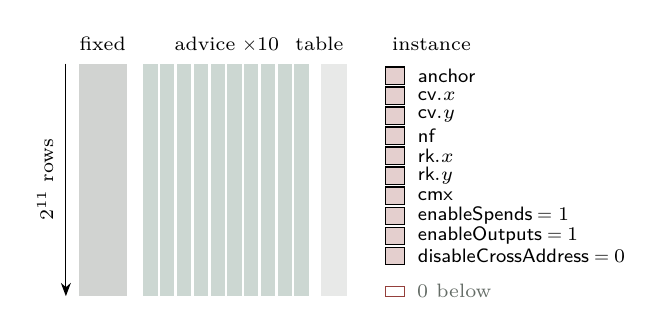
\begin{tikzpicture}[x=0.82cm,y=0.82cm,font=\scriptsize]
  \fill[arbdim!30] (0,0) rectangle ++(0.74,3.6);
  \node[anchor=south] at (0.37,3.65) {fixed};
  \foreach \i in {0,...,9}
    {\fill[arb!25] (1.0+\i*0.26,0) rectangle ++(0.22,3.6);}
  \node[anchor=south] at (2.3,3.65) {advice $\times 10$};
  \fill[arbdim!15] (3.75,0) rectangle ++(0.4,3.6);
  \node[anchor=south east] at (4.25,3.65) {table};
  \foreach \i in {0,...,9}
    {\draw[fill=arbred!25] (4.75,3.28-\i*0.31) rectangle ++(0.3,0.27);}
  \draw[arbred] (4.75,0) rectangle ++(0.3,0.15);
  \node[anchor=south west] at (4.7,3.65) {instance};
  \foreach \i/\l in {0/$\mathsf{anchor}$,1/$\cvsym.x$,2/$\cvsym.y$,
      3/$\nfsym$,4/$\rksym.x$,5/$\rksym.y$,6/$\cmx$,
      7/$\mathsf{enableSpends} = 1$,8/$\mathsf{enableOutputs} = 1$,
      9/$\mathsf{disableCrossAddress} = 0$}
    {\node[anchor=west] at (5.1,3.415-\i*0.31) {\l};}
  \node[anchor=west,text=arbdim] at (5.1,0.075) {$0$ below};
  \draw[-{Stealth}] (-0.2,3.6) -- (-0.2,0)
    node[midway,left=1pt,rotate=90,anchor=south] {$2^{11}$ rows};
\end{tikzpicture}}

\divider{Part F}{The proof system: from a statement to a few kilobytes}

\begin{frame}{A zk-SNARK, precisely enough}
A \emph{relation} $R$ pairs a public statement $x$ with a private witness
$w$; the prover holds both, the verifier only $x$ and a short string:
\[
\mathrm{Prove}(x, w) \to \pi, \qquad
\mathrm{Verify}(x, \pi) \in \{0, 1\}.
\]
\begin{itemize}
  \item \emph{Knowledge sound}: from any prover that convinces the
    verifier, an extractor pulls out a $w$ with $(x, w) \in R$. Plain
    soundness would allow ``a spendable note exists''; other people's
    notes exist. The prover must \emph{hold} one.
  \item \emph{Zero knowledge}: a simulator given only $x$ reproduces
    $\pi$: the proof adds nothing beyond the statement (next slide).
\end{itemize}
A Schnorr signature is a proof of knowledge for the one relation ``I
know $\log_G X$''; a SNARK is the same guarantee for any relation ---
here the ten clauses of the Action statement.
\src{\emph{Crypto Guide}, ``SNARKs: succinct non-interactive arguments of
knowledge''; ``Knowledge soundness and extractors''; ``The simulation
paradigm and zero knowledge''}
\end{frame}

\begin{frame}{Zero knowledge: what $\pi$ hides, and what it does not}
\begin{itemize}
  \item The proof reveals nothing beyond the public inputs: whatever a
    verifier learns from $\pi$, a simulator produces from $x$ alone.
  \item The public inputs ($\nfsym$, $\rksym$, $\cvsym$, $\cmx$) are
    \emph{published}; that they cannot be linked to the note and key
    rests on other assumptions --- commitment hiding, the keyed
    nullifier PRF, key re-randomisation (Parts C and E) --- not on
    $\pi$.
  \item Zero knowledge is necessary, not sufficient: a perfect proof
    beside a nullifier equal to $\cmx$ would hide nothing.
\end{itemize}
Bitcoin's witness is the secret's public shadow (a signature, a script
preimage); here the witness never leaves the prover, and the shadow is
the public-input tuple, unlinkable for reasons the proof does not supply.
\src{\emph{Crypto Guide}, ``The simulation paradigm and zero
knowledge''; \emph{Ironwood Guide}, ``Zero knowledge''}
\end{frame}

\begin{frame}{Succinct, and non-interactive}
\begin{itemize}
  \item \emph{Succinct}: the proof is logarithmic in the circuit
    (commitments and openings, never the polynomials). Halo 2's verifier
    still pays one linear multi-scalar multiplication (MSM), shared across a
    batch; it is a SNARK in the proof-size sense.
  \item \emph{Non-interactive}: wherever a live verifier would toss a
    coin, the prover computes
    \[
    \text{challenge} := \mathrm{Hash}(\text{everything sent so far}),
    \]
    statement and every commitment included --- Fiat--Shamir. A
    commitment is an input of the hash, so it is fixed before the
    challenge that tests it exists. The proof becomes one static object;
    verification recomputes the hashes and runs the same checks.
\end{itemize}
A full node that has never met Alice verifies her Action long after it
was made, from the proof string alone. Schnorr is Fiat--Shamir applied
to the log relation: \emph{proof of knowledge + Fiat--Shamir =
signature}; a SNARK is the same recipe, kept short.
\src{\emph{Crypto Guide}, ``SNARKs: succinct non-interactive arguments of
knowledge''; ``The Fiat--Shamir transform: from interactive to
non-interactive''; \emph{Halo 2 Guide}, ``Removing the verifier: the
Fiat--Shamir transform''}
\end{frame}

% g_toy.py: F_97: omega = 22, H = [1, 22, 96, 75], Z_H = X^4 - 1
%   rows: (3,3,9) (9,3,27) (27,3,30) (30,0,0); every gate equation = 0
\begin{frame}{Arithmetisation: the claim becomes a table}
Toy claim: ``I know $x$ with $x^3 + x + 5 = 35$'' over $\F_{97}$
($x = 3$) --- the Action statement in miniature. One operation per row;
one gate equation, evaluated on every row:
\[
q_M\, a\, b + q_L\, a + q_R\, b + q_O\, c + q_C + \mathrm{PI} = 0
\]
\begin{center}\small
\begin{tabular}{@{}c ccc ccccc c l@{}}
\toprule
& \multicolumn{3}{c}{advice} & \multicolumn{5}{c}{fixed} & instance & \\
\cmidrule(lr){2-4}\cmidrule(lr){5-9}\cmidrule(lr){10-10}
row & $a$ & $b$ & $c$ & $q_M$ & $q_L$ & $q_R$ & $q_O$ & $q_C$
  & $\mathrm{PI}$ & gate \\
\midrule
0 & 3 & 3 & 9 & 1 & 0 & 0 & $-1$ & 0 & 0 & $x \cdot x = x^2$ \\
1 & 9 & 3 & 27 & 1 & 0 & 0 & $-1$ & 0 & 0 & $x^2 \cdot x = x^3$ \\
2 & 27 & 3 & 30 & 0 & 1 & 1 & $-1$ & 0 & 0 & $x^3 + x = s$ \\
3 & 30 & 0 & 0 & 0 & 1 & 0 & 0 & 5 & $-35$ & $s + 5 = 35$ \\
\bottomrule
\end{tabular}
\end{center}
Advice is the prover's secret trace; fixed columns are the circuit;
the instance column carries the public $35$. Copy constraints wire the
rows ($a_0 = b_0 = b_1 = b_2$, $c_0 = a_1$, $c_1 = a_2$, $c_2 = a_3$).
A range check is not algebra: it is a \emph{lookup} into a table.
Bitcoin Script is executed by every validator; a circuit is never
executed, only checked.
\src{\emph{Halo 2 Guide}, ``From computation to a grid of constraints'';
``Proving a value sits in a table: lookups''; ``PLONKish
arithmetisation''}
\end{frame}

% g_toy.py: a(X) coefficients (low degree first) = [90, 61, 22, 24];
%   values on H = [3, 9, 27, 30]; H = [1, 22, 96, 75]; deg G = 9
\begin{frame}{Rows become polynomials}
Name the rows by the fourth roots of unity in $\F_{97}$: $\omega = 22$,
$\omega^2 = 96 = -1$, $\omega^4 = 1$, so row $i$ lives at
$\omega^i \in H = \{1, 22, 96, 75\}$.
\emph{Interpolate} each column: the advice column $a$ is the unique
polynomial of degree $< 4$ through its four values,
\[
a(1) = 3,\ a(22) = 9,\ a(96) = 27,\ a(75) = 30
\quad\Longrightarrow\quad
a(X) = 90 + 61X + 22X^2 + 24X^3 .
\]
Four numbers in, four coefficients out: the column \emph{is} the
polynomial, sampled at the rows. Likewise $b, c$ and the public
$q_M, q_L, q_R, q_O, q_C, \mathrm{PI}$. Substitute into the gate
equation:
\[
G(X) := q_M a b + q_L a + q_R b + q_O c + q_C + \mathrm{PI},
\qquad \deg G \le 9,
\]
and $G(\omega^i)$ is exactly row $i$'s gate equation. So
\[
\text{every gate holds} \iff G(\omega^i) = 0 \text{ for all } i
\iff G \text{ vanishes on } H.
\]
A Merkle root also folds many rows into one object, but it opens one
leaf at a time; a polynomial can be probed anywhere.
\src{\emph{Halo 2 Guide}, ``From the grid to polynomials''}
\end{frame}

% g_toy.py: honest: deg G = 9, deg t = 5, remainder 0
%   cheat c_0 = 10: remainder D = [24, 24, 24, 24], deg D = 3
\begin{frame}{All rows at once: one identity, or none}
The polynomial that is zero exactly on the rows is $\GZH(X) :=
\prod_{h \in H}(X - h) = X^4 - 1$, and by the factor theorem, applied
four times,
\[
G \text{ vanishes on } H
\iff \GZH \mid G
\iff G = t \cdot \GZH \text{ for some polynomial } t .
\]
Honest trace: $\deg G = 9$, $\deg t = 5$, remainder $0$. Now let the
prover claim $x^2 = 10$ and write $c_0 = 10$: row $0$'s gate reads
$3 \cdot 3 - 10 = -1 \neq 0$, so $\GZH \nmid G^{*}$, and for the
Euclidean quotient $t^{*}$
\[
D(X) := G^{*}(X) - t^{*}(X)\, \GZH(X) = 24\,(1 + X + X^2 + X^3) \neq 0 .
\]
A correct computation \emph{is} a polynomial identity; a wrong one
cannot be. The copy constraints get the same treatment (a running
product that equals $1$ when the wiring holds and, at random challenges,
almost never otherwise), and so do lookups.
Bitcoin's validator checks each input's script on its own; here every
row collapses into one identity that holds everywhere or fails almost
everywhere.
\src{\emph{Halo 2 Guide}, ``From vanishing to a single identity'';
``Enforcing the wiring: the permutation argument''}
\end{frame}

% g_toy.py: z = 20: Z_H(z) = 46, t(z) = 67, G(z) = 75, t(z)*Z_H(z) = 75
\begin{frame}{One random point: the protocol}
\begin{enumerate}
  \item The prover \emph{commits} to $a, b, c$ and $t$ (two slides on);
    the verifier already knows $q_M, \dots, q_C$ and $\mathrm{PI}$.
  \item The transcript hash draws $z \in \F$ --- Fiat--Shamir; BLAKE2b
    in the deployed transcript.
  \item The prover opens $a(z), b(z), c(z), t(z)$ with short proofs that
    these are the committed polynomials' values.
  \item The verifier forms $G(z)$ from the openings, computes
    $\GZH(z) = z^4 - 1$, and checks one field equation:
    \[
    G(z) \overset{?}{=} t(z)\, \GZH(z) .
    \]
\end{enumerate}
Honest trace, $z = 20$: $\GZH(20) = 46$, $t(20) = 67$,
$G(20) = 75 = 67 \cdot 46$. \(\checkmark\) Every honest prover passes at
every $z$, because $G = t\,\GZH$ holds as polynomials.

\medskip
Bitcoin's validator re-executes the script; this one evaluates one
equation at one point.
\src{\emph{Halo 2 Guide}, ``Why checking one random point is a proof'';
``Removing the verifier: the Fiat--Shamir transform''; ``The complete
Halo 2 protocol''}
\end{frame}

% g_toy.py: roots of D: [22, 75, 96]; 3/97 = 0.0309; general bound
%   9/97 = 0.0928; cheat at z = 20: G*(z) = 20, t*(z)*Z_H(z) = 64
%   log2(p_Pallas) = 254.000; deg D = 2^14 -> log2(2^14 / p) = -240.0
\begin{frame}{One random point: why a lie is caught}
Cheat: $D := G^{*} - t^{*} \GZH$ is nonzero and \emph{frozen} before
$z$ is drawn --- the commitments pin $G^{*}$ and $t^{*}$. The check
passes exactly when $D(z) = 0$, and a nonzero polynomial has at most
$\deg D$ roots (Schwartz--Zippel), so
\[
\Pr_{z}[\text{cheat accepted}] = \Pr_z[D(z) = 0]
\le \frac{\deg D}{|\F|} .
\]
\begin{itemize}
  \item For the $c_0 = 10$ cheat, $D = 24(1 + X + X^2 + X^3)$ has roots
    $\{22, 75, 96\}$ --- the three rows where the tampered gate still
    held: $3/97$ for that $t^{*}$, $9/97$ for any admissible $t^{*}$.
  \item At $z = 20$: $G^{*}(20) = 20$ but $t^{*}(20)\,\GZH(20) = 64$.
    Caught.
  \item Over $\Fpp$ with $\deg D \approx 2^{14}$ the term is about
    $2^{-240}$ --- one Schwartz--Zippel term, not the system's security
    level; the discrete-log layer gives about $126$ bits.
\end{itemize}
A false statement is too rigid to hide: it disagrees with the truth
almost everywhere, and one probe lands where it disagrees. Bitcoin never
needs this; its validator sees the data.
\src{\emph{Halo 2 Guide}, ``Why checking one random point is a proof'';
\emph{Math Guide}, ``The Schwartz--Zippel lemma''}
\end{frame}

% g_sizes.py: rows = 2^11 = 2048; IPA pair points = 2*log2(2^11) = 22
\begin{frame}{Committing to a polynomial: the problem}
The random-point argument assumed the polynomials were fixed
\emph{before} the random point. Needed: a short commitment $P$ to $f$,
and a short proof that $f(x) = v$ at a drawn point $x$ for the committed
$f$.

\medskip
Commit to the coefficient vector $\vec a$ with a Pedersen vector
commitment, generators $\vec G$ and $H$ hashed into existence:
\[
P = \Comm(f; r) = \ip{\vec a}{\vec G} + [r]\,H \in \G
\]
--- one Vesta point for $2^{11}$ coefficients; binding under discrete
log, hiding by $[r]H$, no secret behind $\vec G$. A Merkle root also
commits to a vector, and opens one entry in $\log_2 d$ hashes; the next
slide opens a linear combination of \emph{all} entries in $2\log_2 d$
points.
\src{\emph{Halo 2 Guide}, ``Why the prover cannot wriggle: binding
commitments''; \emph{Crypto Guide}, ``Polynomial commitment schemes'';
``Hashing to a curve point''}
\end{frame}

\begin{frame}{Committing to a polynomial: the opening claim}
Evaluation is an inner product with a public vector:
\[
f(x) = \ip{\vec a}{\vec b(x)}, \qquad \vec b(x) := (1, x, x^2, \dots,
x^{d-1}) .
\]
Fold the claimed value in with a second hashed generator $U$: the opening
claim becomes
\[
P + [v]\,U = \ip{\vec a}{\vec G} + [r]\,H + [\ip{\vec a}{\vec b}]\,U .
\]
Sending $\vec a$ would cost $d$ elements. The \emph{inner-product
argument} --- the Bulletproofs family you know from range proofs ---
proves the inner product in $2\log_2 d$ points: $22$ for $d = 2^{11}$.
A Merkle proof names one leaf; an IPA opening is one number computed
from every coefficient, at a point chosen after they were fixed.
\src{\emph{Halo 2 Guide}, ``The inner-product polynomial commitment'';
\emph{Crypto Guide}, ``Polynomial commitment schemes''}
\end{frame}

% b_ipa.py: fold check per round: <a',G'> + [r*]H + [<a',b'>]U equals
%   acc + [u^2]L + [u^-2]R (round 2: 25 = 25; round 1: 12 = 12)
\begin{frame}{The inner-product argument: one fold}
Split every vector in half, $\vec a = (\Glo{\vec a}, \Ghi{\vec a})$,
likewise $\vec G$ and $\vec b$, and publish the two cross terms
\begin{align*}
L &:= \ip{\Glo{\vec a}}{\Ghi{\vec G}} + [\ell]\,H
      + [\ip{\Glo{\vec a}}{\Ghi{\vec b}}]\,U, \\
R &:= \ip{\Ghi{\vec a}}{\Glo{\vec G}} + [r_R]\,H
      + [\ip{\Ghi{\vec a}}{\Glo{\vec b}}]\,U .
\end{align*}
Draw a challenge $u$ and fold, both parties in step:
\[
\vec a' := u\,\Glo{\vec a} + u^{-1}\Ghi{\vec a}, \quad
\vec G' := u^{-1}\Glo{\vec G} + u\,\Ghi{\vec G}, \quad
\vec b' := u^{-1}\Glo{\vec b} + u\,\Ghi{\vec b} .
\]
Multiply out: $\ip{\vec a'}{\vec G'} = \ip{\vec a}{\vec G} +
u^2 \ip{\Glo{\vec a}}{\Ghi{\vec G}} + u^{-2} \ip{\Ghi{\vec a}}{\Glo{\vec
G}}$, and the same for $\ip{\vec a'}{\vec b'}$. Hence
\[
P + [v]\,U + [u^2]\,L + [u^{-2}]\,R
= \ip{\vec a'}{\vec G'} + [r + u^2 \ell + u^{-2} r_R]\,H
  + [\ip{\vec a'}{\vec b'}]\,U :
\]
the same claim at half the length. The verifier updates $\vec G'$ and
$\vec b'$ by public arithmetic and never sees $\vec a$. This is the
textbook (Bulletproofs) form; a Bulletproofs range proof folds its
vectors by exactly this move.
\src{\emph{Halo 2 Guide}, ``The inner-product polynomial commitment'',
Construction ``IPA-based polynomial commitment''}
\end{frame}

% g_sizes.py: IPA pair points = 22; IPA group elements = 2*11 + 1 = 23
\begin{frame}{The inner-product argument: the recursion}
After $k = \log_2 d$ rounds every vector has length $1$. The proof is
$2k$ points $(L_j, R_j)$, the final scalar $a$, and the aggregated
blinder $r^{*} = r + \sum_j (u_j^2 \ell_j + u_j^{-2} r_j)$. The verifier
accepts iff
\[
P + [v]\,U + \sum_{j=1}^{k}\bigl([u_j^2]\,L_j + [u_j^{-2}]\,R_j\bigr)
\overset{?}{=} [a]\,G^{(0)} + [r^{*}]\,H + [a \cdot b^{(0)}]\,U .
\]
\begin{itemize}
  \item The scalar $b^{(0)} = \prod_{\ell}(u_\ell^{-1} + u_\ell\,
    x^{2^{\ell-1}})$ costs $O(\log d)$ field operations.
  \item The point $G^{(0)} = \ip{\vec s}{\vec G}$ is a multi-scalar
    multiplication of length $d$ --- the one linear step. The node shares
    it across a batch; recursion would defer it into an accumulator (not
    deployed).
  \item \emph{Binding}: two openings of one commitment would exhibit a
    non-trivial discrete-log relation among $\vec G, H$ on \Vesta; an
    extractor rewinds three challenges per round.
\end{itemize}
A Bitcoin signature check costs a fixed handful of group operations; an
IPA opening is logarithmic in size but ends in a circuit-sized wall of
group arithmetic.
\src{\emph{Halo 2 Guide}, ``The inner-product polynomial commitment'';
``Accumulation and the Halo trick''; \emph{Crypto Guide}, ``Polynomial
commitment schemes''}
\end{frame}

\begin{frame}{What the fold hides, and the deployed normalisation}
\begin{itemize}
  \item Folding alone is \emph{not} zero knowledge: the final scalar
    $a$ is a challenge-dependent linear form in the coefficients, and
    blinding $P$ and the round points hides those points, not $a$.
  \item The deployed opening first masks $f$ by a random polynomial
    vanishing at the opening point, commits to it as $S$, draws two
    further challenges, and only then folds.
  \item The deployed fold is rescaled: weights $(1, u_j^{-1})$ on the
    coefficients, $(1, u_j)$ on $\vec b$ and $\vec G$, the verifier
    accumulating $[u_j^{-1}]\,L_j + [u_j]\,R_j$; the two conventions
    are related by per-round rescaling.
\end{itemize}
The slides' $[u^2]L + [u^{-2}]R$ form is the textbook one; the deployed
proof carries the same $2k$ points plus $S$ and two final scalars. A
Bitcoin signature exposes its public key by design; here even the last
scalar of an opening must be masked.
\src{\emph{Halo 2 Guide}, ``The inner-product polynomial commitment'',
Remarks ``Folding alone is not zero knowledge'', ``The deployed IPA
normalisation''}
\end{frame}

% b_ipa.py: a = [5, 1, 0, 1], x = 3, b = [1, 3, 9, 27], v = 35
%   G = [2, 3, 5, 7], H = 11, U = 13, r = 17; P = <a,G> + r*H = 13
%   round 2: L_2 = 13, R_2 = 4, u_2 = 3; a^(1) = [15, 68], b^(1) = [92, 82],
%     G^(1) = [48, 22]; fold check 25 = 25, r* = 72
%   round 1: L_1 = 52, R_1 = 58, u_1 = 5; a^(0) = [11], b^(0) = [21],
%     G^(0) = [42]; fold check 12 = 12, r* = 30
\begin{frame}{The fold by hand: two rounds}
The Halo 2 Guide's symbolic $d = 4$ example with numbers: the toy
$p(X) = 5 + X + X^3$ opened at $x = 3$, so $v = 35$. Stand-in group
$\mathbb{Z}_{97}$ written additively --- a ``point'' is a residue and $[k]G = kG
\bmod 97$; it has no discrete-log hardness, only the fold's algebra.
\begin{align*}
\vec a &= (5, 1, 0, 1), &
\vec b &= (1, 3, 9, 27), &
\vec G &= (2, 3, 5, 7), \\
H &= 11, & U &= 13, & r &= 17,
\qquad P = \ip{\vec a}{\vec G} + [r]H = 13 .
\end{align*}
\begin{center}\small
\begin{tabular}{@{}l ccc ccc c@{}}
\toprule
round & $L_j$ & $R_j$ & $u_j$ & $\vec a'$ & $\vec b'$ & $\vec G'$
  & fold check \\
\midrule
$j = 2$ ($\ell_2, r_2 = 19, 23$) & $13$ & $4$ & $3$ & $(15, 68)$ & $(92, 82)$
  & $(48, 22)$ & $25 = 25$ \\
$j = 1$ ($\ell_1, r_1 = 29, 31$) & $52$ & $58$ & $5$ & $(11)$ & $(21)$
  & $(42)$ & $12 = 12$ \\
\bottomrule
\end{tabular}
\end{center}
Each row's fold check is the one-fold identity: the folded
claim $\ip{\vec a'}{\vec G'} + [r^{*}]H + [\ip{\vec a'}{\vec b'}]U$ equals
the accumulated $P + [v]U + [u^2]L + [u^{-2}]R$.
\src{\emph{Halo 2 Guide}, ``The inner-product polynomial commitment''}
\end{frame}

% b_ipa.py: final: a = 11, r* = 30, b^(0) = 21, G^(0) = 42
%   LHS P + [v]U + sum([u_j^2]L_j + [u_j^-2]R_j) = 12; RHS = 12; equal
%   s = [13, 34, 20, 15]: <s,G> = 42 = G^(0); g(x;u1,u2) = 21 = b^(0)
\begin{frame}{The fold by hand: the final check}
The prover sends $a = 11$ and $r^{*} = 30$. From the challenges alone
the verifier computes
\begin{gather*}
\vec s = (u_1^{-1}u_2^{-1},\ u_1 u_2^{-1},\ u_1^{-1}u_2,\ u_1 u_2)
= (13, 34, 20, 15), \qquad G^{(0)} = \ip{\vec s}{\vec G} = 42, \\
b^{(0)} = g(x; u_1, u_2) = (u_1^{-1} + u_1 x)(u_2^{-1} + u_2 x^2) = 21,
\end{gather*}
and compares the two sides:
\begin{align*}
P + [v]U + [u_1^2]L_1 + [u_1^{-2}]R_1 + [u_2^2]L_2 + [u_2^{-2}]R_2
  &= 12, \\
[a]\,G^{(0)} + [r^{*}]\,H + [a \cdot b^{(0)}]\,U &= 12 .
\end{align*}
Equal: accepted. Four coefficients were never sent; four points and two
scalars were. In $\mathbb{Z}_{97}$ anyone can divide, so nothing here is
hidden or binding; on \Vesta{} the same equations are, and $G^{(0)}$ is
a length-$2^{11}$ multi-scalar multiplication.
\src{\emph{Halo 2 Guide}, ``The inner-product polynomial commitment''}
\end{frame}

\begin{frame}{Fields and curves in the deployed circuit}
\begin{itemize}
  \item The circuit's native field is $\Fpp$, the \emph{base} field of
    \Pallas: the points the statement handles --- $\cmsym$, $\rksym$,
    $\cvsym$, $\aksym$, $\pkd$ --- have coordinates there, so the group
    law is native arithmetic, not emulated.
  \item The column polynomials are committed on \Vesta, whose
    \emph{scalar} field is exactly $\Fpp$: the coefficients are the
    circuit's own field elements.
\end{itemize}
Bitcoin's secp256k1 is one curve doing one job: its validator verifies
signatures, never circuits. And its base field, as the two-adicity slide
shows, cannot even host the prover's evaluation domain.
\src{\emph{Ironwood Guide}, ``Flags, public inputs, and circuit
parameters''; \emph{Math Guide}, ``Base fields, scalar fields, and the
Pasta cycle''}
\end{frame}

\begin{frame}{The Pasta cycle, once}
\Pallas{} over $\Fpp$ has order $p_{\Vesta}$; \Vesta{} over $\Fpv$ has
order $p_{\Pallas}$: each curve's scalar field is the other's base field.
\begin{itemize}
  \item A Vesta-committed proof is Vesta points with coordinates in
    $\Fpv$, Pallas's scalar field; the circuit that verifies it natively
    is one over $\Fpv$, committed on Pallas.
  \item That circuit's proof is Pallas points with coordinates in
    $\Fpp$, verified natively by a circuit over $\Fpp$, committed on
    Vesta --- proofs alternate between the two curves, each verifier a
    circuit, so one proof can attest to the previous one.
  \item Not deployed: the node verifies each bundle's proof directly and
    batches the deferred multi-scalar multiplications.
\end{itemize}
Bitcoin needs no such pair; a signature is verified by arithmetic, not
by another proof.
\src{\emph{Halo 2 Guide}, ``A cycle of curves for efficient native
recursion''; ``Accumulation and the Halo trick''; \emph{Math Guide},
``Base fields, scalar fields, and the Pasta cycle''}
\end{frame}

% g_twoadic.py: Pallas base 255 bits, two-adicity 32, domain 2^32, hosts
%   2^11 rows: True; Vesta base 255 bits, 32, 2^32, True; secp256k1 base
%   256 bits, 1, 2^1 = 2, False; secp256k1 scalar 256 bits, 6, 2^6 = 64,
%   False
\begin{frame}{Why not Bitcoin's curve: two-adicity}
Interpolating a column over $n = 2^{11}$ rows needs a primitive
$2^{11}$-th root of unity, hence $2^{11} \mid p - 1$; the prover's
quotient FFTs run on $8n = 2^{14}$ points at the deployed gate degree.
The largest $k$ with $2^k \mid p - 1$ is the field's \emph{two-adicity}.
{\centering\small
\begin{tabular}{@{}lccc@{}}
\toprule
field & bits & two-adicity of $p - 1$ & largest domain \\
\midrule
$\Fpp$ (Pallas base) & $255$ & $32$ & $2^{32}$ \\
$\Fpv$ (Vesta base) & $255$ & $32$ & $2^{32}$ \\
secp256k1 base field & $256$ & $1$ & $2$ \\
secp256k1 scalar field & $256$ & $6$ & $64$ \\
\bottomrule
\end{tabular}\par}
\smallskip
The Pasta primes were designed with two-adicity exactly $32$
(\emph{Math Guide}; their values: protocol specification, ``Pallas and
Vesta''): domains of every size up to $2^{32}$. Bitcoin's curve buys its
implementation speed from $a = 0$ (\emph{Crypto Guide}); its prime
$p = 2^{256} - 2^{32} - 977$ was not chosen for evaluation domains:
$p - 1$ is twice an odd number, a domain of two points. The secp256k1
rows are this deck's own computation, not a volume figure.
\src{\emph{Math Guide}, ``Pallas and Vesta assembled'', Remark
``Two-adicity and FFT-friendly primes''; \emph{Crypto Guide}, ``The
transparent layer's schemes: ECDSA and BIP-340 over secp256k1'';
\emph{Halo 2 Guide}, ``The complete Halo 2 protocol''}
\end{frame}

\begin{frame}{Trust: what a ceremony is, and why there is none}
\small
Pairing SNARKs (Sapling's Groth16) bake a secret into the parameters;
the pairing-based polynomial commitment (KZG, after Kate, Zaverucha and
Goldberg) shows the shape:
\[
pp = \bigl([\tau^0]G, [\tau^1]G, \dots, [\tau^d]G, \dots\bigr),
\qquad \tau \text{ destroyed.}
\]
Whoever keeps $\tau$ forges: for any $C$, $z$, $y$ the element
$\pi := [(\tau - z)^{-1}]\,(C - [y]G)$ passes the check with no
polynomial behind it --- the \emph{toxic waste}. Groth16's secrets are
per circuit. A multiparty ceremony keeps the waste unknown provided
\emph{one} participant destroyed their share; the Sapling pool still
rests on that.

\smallskip
The bound: under ZIP-209 each pool's chain value balance is public and
may not go negative, so a forged Sapling proof creates value only
inside the Sapling pool and can withdraw at most what that pool
publicly holds --- the turnstile (Part H).

\smallskip
Orchard and Ironwood: the IPA generators are hashed from a public
domain tag, nothing to leak, nothing to destroy; binding rests on
discrete log alone. Bitcoin never had a setup; Sapling has one; Orchard
returns to none.
\src{\emph{Crypto Guide}, ``Polynomial commitment schemes''; ``SNARKs:
succinct non-interactive arguments of knowledge''; \emph{Halo 2 Guide},
``The ``Halo'' in Halo 2: deferring the expensive check'';
\emph{Ironwood Guide}, ``Pool balances: ZIP-209 and its Ironwood
analogue''}
\end{frame}

% g_sizes.py: BCTV14 = 7*33 + 65 = 296 B; Groth16 = 2*48 + 96 = 192 B
%   Halo 2: 2720 + 2272*1 = 4992 B; 2720 + 2272*2 = 7264 B
\begin{frame}{Three generations}
{\centering\small
\begin{tabular}{@{}llll@{}}
\toprule
& Sprout & Sapling & Orchard, Ironwood \\
\midrule
SNARK & BCTV14 (original) & Groth16 & Halo 2 \\
curve & BN254 & BLS12-381, Jubjub in-circuit & Pallas, Vesta \\
setup & six-party MPC & large MPC & none \\
hash in circuit & SHA-256 & Pedersen & Sinsemilla \\
proof & 296 B & 192 B & $2720 + 2272a$ B \\
verification & constant & three pairings & $O(\log n)$ + shared MSM \\
\bottomrule
\end{tabular}\par}
A soundness flaw in BCTV14, found after deployment, would have allowed
undetected counterfeiting; Sprout was re-proved with Groth16 and
deprecated. Sapling: Groth16 over BLS12-381, Jubjub inside the circuit;
a far faster prover, a per-circuit ceremony, no curve cycle. Orchard's
proof grew because transparency costs $2\log_2 n$ points.
Bitcoin changed its signature scheme once, by opt-in; Zcash has carried
shielded payments through three proof systems, each with its own pool
--- the third with two, Orchard and Ironwood, on one circuit.
\src{\emph{Ironwood Guide}, ``Lineage: three generations of shielded
proof''; ``Comparative summary''}
\end{frame}

% g_sizes.py: rows = 2^11 = 2048; advice columns = 10; IPA pair points
%   = 22; IPA group elements = 23; proof 4992 B (a = 1), 7264 B (a = 2);
%   signature 64 B; 4992 / 64 = 78; Action encoding 820 B
\begin{frame}{The Orchard circuit by the numbers}
\begin{center}\small
\begin{tabular}{@{}ll@{}}
\toprule
rows & $2^{11} = 2048$; one fixed circuit, every Action an instance \\
columns & ten advice, fixed columns, a Sinsemilla lookup table \\
proof per bundle & $2720 + 2272\,a$ B: $4992$ for one Action, $7264$
  for Alice's two \\
of which IPA & $22$ pair points and one blinding commitment, $32$ B
  each \\
proving & a few seconds on commodity hardware \\
verifying & $O(\log n)$ per proof, plus one MSM shared across a batch \\
\bottomrule
\end{tabular}
\end{center}
One aggregate proof covers all of a bundle's Actions; the per-Action
term is that Action's column commitments and evaluations, the constant
term the shared quotient, multipoint, and IPA data. A spend-auth
signature is $64$ bytes; a one-Action proof is $78$ signatures' worth.
Bitcoin's witness cost is per input and grows with the script it
satisfies; here it is per bundle, logarithmic in the circuit, and
independent of the anonymity set.
\src{\emph{Ironwood Guide}, ``Flags, public inputs, and circuit
parameters''; ``The v6 transaction and the Ironwood component'';
\emph{Halo 2 Guide}, ``The complete Halo 2 protocol''}
\end{frame}

\begin{frame}{Five gadget families, three circuit versions}
\begin{itemize}
  \item \emph{ECC}: the Pallas group law --- $\rksym = \aksym +
    [\alpha]\,G^{\mathsf{SpendAuth}}$ (A6), $\pkd = [\ivk]\,\gd$ (A7),
    $\cvsym$ (A4), the nullifier's point (A5).
  \item \emph{Sinsemilla}: the generator table as a lookup; each
    $10$-bit chunk costs one lookup and two incomplete additions;
    carries $\NoteCommit$ (A1, A2) and $\CommitIvk$ (A7).
  \item \emph{Merkle path}: $32$ layer-tagged hashes, a conditional swap
    per layer by one bit of the position, root $=$ anchor gated by
    $v_{\mathrm{old}}$ (A3).
  \item \emph{Poseidon}: the nullifier PRF; its only non-linearity is
    $x \mapsto x^5$ (A5).
  \item \emph{Decomposition}: range checks $v \in [0, 2^{64})$ and the
    sign bit (A4); canonicity of witnessed point and field-element
    encodings --- distinct from the node's parsing of public encodings
    (Part E).
\end{itemize}
Three Action-circuit versions exist --- the original, a correction, the
Ironwood circuit with the cross-address input --- and consensus selects
the verifying key by branch, so every Action in either pool now verifies
against the Ironwood key. Bitcoin's validator runs whatever script an
output declares; this one runs a verifier keyed to one fixed circuit.
\src{\emph{Ironwood Guide}, ``The gadget set''; ``One circuit, one
verifying key''}
\end{frame}

% Ironwood Guide, "The Action statement, formally": eight named public
%   inputs; instance elements 1+2+1+2+1+1+1+1 = 10; disableCrossAddress
%   at index 9. ep_actions.py: per-Action sums +50000000 (Action 1).
%   g_sizes.py: rows = 2^11 = 2048
\begin{frame}{Alice's Action as an instance}
\begin{columns}[c]
\begin{column}{0.6\textwidth}
\centering
\GInstanceFig
\end{column}
\begin{column}{0.4\textwidth}
\small
\textbf{Instance} (Action 1: $2$ ZEC $\to$ Bob $1.5$): eight public
inputs, ten field elements; the two points enter by coordinates; the
flags as the Ironwood component sets them.

\medskip
\textbf{Advice}: both notes; $32$ siblings and the position;
$\aksym$, $\nksym$, $\rivk$, $\ivk$; $\alpha$; $\rcv$;
$(\mathrm{magnitude}, \mathrm{sign}) = (50\,000\,000, +1)$.

\medskip
Copy constraints tie each instance cell to the advice cell holding the
same value; the verifier computes the instance commitment itself, so a
proof for other values fails the opening.
\end{column}
\end{columns}
Bitcoin's witness (scriptSig or witness field) is in the clear; here
the witness fills advice cells nobody reads.
\src{\emph{Ironwood Guide}, ``The Action statement, formally'';
\emph{Halo 2 Guide}, ``Instance columns and binding the public
statement''}
\end{frame}

\begin{frame}{Checkpoint}
\Large
What could a holder of the Sapling ceremony's toxic waste do, what
stops the analogue in Orchard, and what bounds the damage?
\pause
\normalsize
\medskip
\begin{itemize}
  \item Forge accepting Sapling proofs of false statements:
    counterfeit inside the Sapling pool, invisible to every verifier.
    Not decrypt notes --- soundness and zero knowledge are separate
    guarantees.
  \item In Orchard there is no trapdoor to hold: the generators are
    hashed, and binding reduces to discrete log.
  \item Under ZIP-209 each pool's chain value balance is public, and a
    block that would drive it negative is invalid --- counterfeit is
    capped at the pool's exit.
\end{itemize}
\src{\emph{Crypto Guide}, ``SNARKs: succinct non-interactive arguments of
knowledge''; \emph{Ironwood Guide}, ``Pool balances: ZIP-209 and its
Ironwood analogue''}
\end{frame}

%% ---- 08-delivery.tex
%% Part F --- Delivery and light clients
%% Sources: Ironwood Guide "Minting: a note is born" (the note seed and the
%% Ironwood trapdoor), "Delivery: the note reaches its owner" (both
%% ciphertexts, trial decryption, synchronisation), "Resting: the note in
%% the commitment tree" (shards, cap, anchors); Wallet Guide "Compact blocks
%% (ZIP-307)", "Commitment-tree synchronisation", "What the server learns";
%% Wallet Guide "Internal keys: change and auto-shielding", "Transaction
%% construction", "Broadcast, expiry, and the transaction lifecycle".
%% Numbers: compute/f_delivery.py, compute/f_lightclient.py, compute/f_rcm.py.
%% Uses no shared figure macro.

\newcommand{\Fenc}{\ensuremath{C_{\mathrm{enc}}}}
\newcommand{\Fout}{\ensuremath{C_{\mathrm{out}}}}
\newcommand{\Fnp}{\ensuremath{\mathsf{np}}}
\newcommand{\Frseed}{\ensuremath{\mathsf{rseed}}}
\newcommand{\Fock}{\ensuremath{\mathsf{ock}}}
\newcommand{\Fpre}{\ensuremath{\mathsf{pre}_{\rcm}}}
\newcommand{\Fivkint}{\ensuremath{\ivk^{\mathsf{int}}}}
\newcommand{\Fkenc}{\ensuremath{K_{\mathrm{enc}}}}

\divider{Part G}{Delivery and light clients}

%% compute/f_delivery.py:
%% compact note plaintext = 1+11+8+32 = 52 B
%% full note plaintext    = 52+512 = 564 B
%% compute/f_rcm.py:
%% PRFexpand calls per note = 3 (esk, psi, rcm), all keyed by the 32-byte rseed
\begin{frame}{The note plaintext: what travels to Bob}
The chain stores \cmx; the note itself must still reach Bob. What Alice
sends him is the \emph{note plaintext}
\[
\Fnp := (\mathtt{0x03},\ d,\ v,\ \Frseed,\ \mathsf{memo}),
\qquad 1 + 11 + 8 + 32 + 512 = 564 \text{ bytes.}
\]
\begin{itemize}
  \item The lead byte names the format: $\mathtt{0x03}$ is the Ironwood
    note, the only value the Ironwood pool admits.
  \item The $32$-byte seed \Frseed{} is the note's whole randomness. Three
    $\mathsf{PRFexpand}$ calls keyed by it, each under its own domain
    byte, yield \esk{} ($\mathtt{0x04} \,\|\, \rho$), $\psi$
    ($\mathtt{0x09} \,\|\, \rho$), and \rcm{} (next slide); with
    $\rho := \nfsym_{\mathrm{old}}$, the seed is bound to its Action.
  \item The memo is $512$ bytes of sender-chosen data, encrypted with the
    rest; it never appears in the clear.
  \item \emph{Bitcoin contrast:} an output shows its amount and script to
    everyone, and an OP\_RETURN note is public.
\end{itemize}
\src{\emph{Ironwood Guide}, ``Sender: one-shot Diffie--Hellman and the
  AEAD''; ``The note seed: Ironwood derivations (lead byte $\mathtt{0x03}$)'';
  protocol specification, ``Note Plaintexts and Memo Fields''}
\end{frame}

%% compute/f_rcm.py:
%% pre_rcm = 1+32+32+8+32+32 = 137 B (0x0B-separated)
%% legacy rcm input = 1+32 = 33 B (0x05 || rho)
\begin{frame}{The Ironwood trapdoor: one hash over every note field}
The one note-level difference between the pools: how \rcm{} leaves the
seed.
\begin{align*}
\text{Ironwood pool } (\mathtt{0x03}):&\quad
\rcm := \mathrm{ToScalar}\bigl(\mathsf{PRFexpand}_{\Frseed}(\Fpre)\bigr),\\
&\quad \Fpre := \mathtt{0x0B} \,\|\, \gd^\star \,\|\, \pkd^\star \,\|\,
  \mathrm{LE}_{64}(v) \,\|\, \mathrm{LE}_{256}(\rho) \,\|\,
  \mathrm{LE}_{256}(\psi),\\
\text{Orchard pool } (\mathtt{0x02}):&\quad
\rcm := \mathrm{ToScalar}\bigl(\mathsf{PRFexpand}_{\Frseed}(
  \mathtt{0x05} \,\|\, \mathrm{LE}_{256}(\rho))\bigr).
\end{align*}
\begin{itemize}
  \item A $1 + 32 + 32 + 8 + 32 + 32 = 137$-byte preimage against $33$:
    every note field enters the trapdoor, so \rcm{} is derived last, after
    $\psi$. The commitment itself is unchanged: same \NoteCommit, same
    tree construction --- each pool its own instance (ZIP-229).
  \item Both pools' notes carry \esk{} and $\psi$ byte-identically; only
    the trapdoor differs, and the lead byte says which derivation
    applies.
  \item \emph{Bitcoin contrast:} a Bitcoin output has no trapdoor at all
    --- there is nothing hidden to bind.
\end{itemize}
\src{\emph{Ironwood Guide}, ``The note seed: Ironwood derivations (lead
  byte $\mathtt{0x03}$)''; ``Lead bytes across pools and the legacy
  derivation''}
\end{frame}

\begin{frame}{Why the detour through BLAKE2b: post-quantum binding}
\begin{itemize}
  \item The commitment's binding is Sinsemilla collision resistance ---
    a discrete-log assumption, which a large quantum computer breaks
    (Part I). Once it falls, \NoteCommit{} alone binds nothing.
  \item Model $\mathsf{PRFexpand}$ as a random oracle. Every field enters
    $\Fpre$, so any change to a committed note re-randomises \rcm; landing
    two honestly derived note--trapdoor pairs on one commitment is a
    collision event in the oracle, with no group structure for Shor.
  \item The composite of derivation and \NoteCommit{} is therefore
    post-quantum binding --- \emph{provided a verifier checks the
    derivation}. No deployed Action clause does; the claim is conditional
    on that future check.
  \item This is what makes an Ironwood note \emph{recoverable}, and no
    Orchard- or Sapling-pool note. Parts H and I return to it.
  \item \emph{Bitcoin contrast:} nothing in a Bitcoin output is hidden,
    so nothing must stay bound after a break; here the hidden note must.
\end{itemize}
\src{\emph{Ironwood Guide}, ``The note seed: Ironwood derivations (lead
  byte $\mathtt{0x03}$)''; ``ZIP-2005: quantum recoverability''}
\end{frame}

%% compute/f_delivery.py:
%% full note plaintext    = 52+512 = 564 B
%% C_enc = 564+16 = 580 B;  C_out = 64+16 = 80 B
\begin{frame}{Sealing the note: one-shot Diffie--Hellman, then an AEAD}
Alice holds Bob's address $(d, \pkd)$, where $\pkd = [\ivk]\,\gd$ and
$\gd = \GroupHash(d)$. With \esk{} drawn from \Frseed{} she runs a key
agreement to the diversified base:
\begin{gather*}
\epk := [\esk]\,\gd, \qquad
\mathsf{s} := [\esk]\,\pkd, \qquad
\Fkenc := \mathsf{KDF}(\mathsf{s},\ \epk),\\
\Fenc := \mathsf{Enc}_{\Fkenc}(\Fnp)
\qquad (564 + 16\text{-byte tag} = 580 \text{ bytes}).
\end{gather*}
\begin{itemize}
  \item The KDF is BLAKE2b-256 over the encodings of $\mathsf{s}$ and
    \epk; the AEAD is ChaCha20-Poly1305 under a fixed all-zero nonce and
    empty associated data --- a fresh key for every note.
  \item Why Bob: $[\ivk]\,\epk = [\ivk][\esk]\,\gd = [\esk]\,\pkd =
    \mathsf{s}$, so the holder of \ivk{} --- and the sender, who knows
    \esk{} --- recovers \Fkenc{} from the published pair $(\epk, \Fenc)$.
  \item \emph{Bitcoin contrast:} BIP-352 runs the same ECDH with the
    input keys standing in for \esk{} --- no \epk{} is published --- to
    derive an output key the chain then shows in the clear; here the
    shared secret encrypts the note, amount and memo included.
\end{itemize}
\src{\emph{Ironwood Guide}, ``Sender: one-shot Diffie--Hellman and the
  AEAD''; protocol specification, ``In-band secret distribution (Sapling
  and Orchard)''}
\end{frame}

%% compute/f_delivery.py:
%% C_enc = 564+16 = 580 B;  C_out = 64+16 = 80 B
\begin{frame}{The second ciphertext: the sender's own copy}
One ciphertext serves Bob; a second can serve Alice's books. Given an
outgoing viewing key, the pair $(\pkd, \esk)$ is sealed under the
\emph{outgoing cipher key}:
\[
\Fock := \mathrm{BLAKE2b\text{-}256}\bigl(\ovk \,\|\, \cvsym \,\|\,
  \cmx \,\|\, \epk\bigr), \qquad
\Fout := \mathsf{Enc}_{\Fock}(\pkd,\ \esk).
\]
\begin{itemize}
  \item From $(\pkd, \esk)$ the holder of \ovk{} re-derives
    $\mathsf{s} = [\esk]\,\pkd$ and reads the note as Bob does: $64 + 16
    = 80$ bytes buy a sent history.
  \item Binding \cvsym, \cmx, \epk{} into the key pins \Fout{} to its own
    Action; with $\ovk = \bot$ the sender seals random bytes under a
    random key instead, and no outgoing key ever opens it.
  \item The Action publishes $(\epk, \Fenc, \Fout)$ beside
    $\cvsym, \nfsym, \rksym, \cmx$; the node never opens the three, and
    no clause of the Action statement mentions them.
  \item \emph{Bitcoin contrast:} a Bitcoin sender needs no copy --- the
    chain is the copy; here a wallet's sent history exists only if it
    kept a key that reads it.
\end{itemize}
\src{\emph{Ironwood Guide}, ``The outgoing ciphertext''; ``What a node
  verifies, without ever observing the note''; protocol specification,
  ``Decryption using an Outgoing Viewing Key (Sapling and Orchard)''}
\end{frame}

\begin{frame}{Finding your money: detection is successful decryption}
Nothing on chain names a recipient, so Bob's wallet trial-decrypts
\emph{every} Orchard-protocol output with \ivk:
\[
\mathsf{s} := [\ivk]\,\epk, \qquad
\Fkenc := \mathsf{KDF}(\mathsf{s},\ \epk), \qquad
\Fnp := \mathsf{Dec}_{\Fkenc}(\Fenc).
\]
\begin{itemize}
  \item The AEAD tag rejects a wrong key; an open is a \emph{candidate},
    not yet a note.
  \item Two re-derivations close the obvious forgeries: \esk{} from
    \Frseed{} must give $[\esk]\,\gd = \epk$, and the note rebuilt from
    $(d, v, \Frseed)$ and the Action's own $\rho := \nfsym_{\mathrm{old}}$
    must give $\Extract(\NoteCommit_{\rcm}(\ldots)) = \cmx$.
  \item The cost: one key agreement per output for each \ivk, plus the
    bandwidth of every output. One \ivk{} scans both pools.
  \item \emph{Bitcoin contrast:} a Bitcoin wallet asks for its addresses'
    outputs, a lookup over public scripts; here no field on chain names
    the recipient, so there is nothing to ask for.
\end{itemize}
\src{\emph{Ironwood Guide}, ``Recipient: trial decryption and
  re-derivation''; \emph{Wallet Guide}, ``Compact blocks (ZIP-307)'';
  protocol specification, ``Decryption using an Incoming Viewing Key
  (Sapling and Orchard)''}
\end{frame}

%% compute/f_delivery.py:
%% compact note plaintext = 1+11+8+32 = 52 B
%% full note plaintext    = 52+512 = 564 B
%% C_enc = 564+16 = 580 B;  C_out = 64+16 = 80 B
%% dropped from C_enc by compaction = 528 B (memo + tag)
%% compact Action = 3*32+52 = 148 B of 820 B (18%)
\begin{frame}{Compact blocks (ZIP-307): what a light client downloads}
\centering
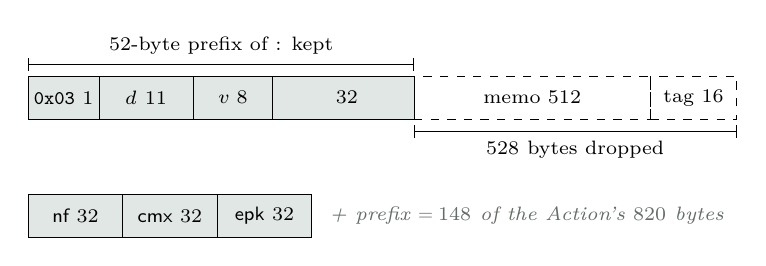
\begin{tikzpicture}[every node/.style={font=\scriptsize},
  b/.style={draw,minimum height=5.5mm,inner sep=2pt,outer sep=0pt,
    anchor=west}]
\node[b,fill=arb!15,minimum width=9mm] (l) at (0,0) {$\mathtt{0x03}$ 1};
\node[b,fill=arb!15,minimum width=12mm] (d) at (l.east) {$d$ 11};
\node[b,fill=arb!15,minimum width=10mm] (v) at (d.east) {$v$ 8};
\node[b,fill=arb!15,minimum width=18mm] (r) at (v.east) {\Frseed{} 32};
\node[b,dashed,minimum width=30mm] (m) at (r.east) {memo 512};
\node[b,dashed,minimum width=11mm] (t) at (m.east) {tag 16};
\draw[|-|] ([yshift=1.5mm]l.north west) -- ([yshift=1.5mm]r.north east)
  node[midway,above] {$52$-byte prefix of \Fenc: kept};
\draw[|-|] ([yshift=-1.5mm]m.south west) -- ([yshift=-1.5mm]t.south east)
  node[midway,below] {$528$ bytes dropped};
\node[b,fill=arb!15,minimum width=12mm] (nf) at (0,-1.5) {\nfsym{} 32};
\node[b,fill=arb!15,minimum width=12mm] (cm) at (nf.east) {\cmx{} 32};
\node[b,fill=arb!15,minimum width=12mm] (ep) at (cm.east) {\epk{} 32};
\node[anchor=west,font=\scriptsize\itshape,text=arbdim] at (ep.east)
  {\ + prefix $= 148$ of the Action's $820$ bytes};
\end{tikzpicture}
\par\medskip
\begin{itemize}
  \item A compact block keeps only what three tasks need: detect a
    payment, detect a spend of one's own notes, update witnesses.
  \item Per Action: \nfsym, \cmx, \epk, and the prefix. Dropped: memo,
    tag, \Fout, \cvsym, \rksym, anchor, proof, signatures. Each block
    also states its end-of-block tree size per pool.
  \item \emph{Bitcoin contrast:} an SPV client downloads headers and asks
    for what matches; this client downloads every compact block in range
    and asks for no particular output.
\end{itemize}
\src{\emph{Wallet Guide}, ``Compact blocks (ZIP-307)''; ``The deployed
  messages''; ``Omissions and fetch-on-detect''; \emph{Ironwood Guide},
  ``Synchronisation, including from cold storage''}
\end{frame}

%% compute/f_delivery.py:
%% compact note plaintext = 1+11+8+32 = 52 B
%% compact decryption: keystream bytes [64..116) after skipping block 0 (64 B)
\begin{frame}{Accepting a note without its tag}
Truncation at $52$ bytes discards the Poly1305 tag, so a compact
decryption cannot be authenticated the AEAD way:
\[
\Fnp := \mathsf{ciphertext}[0..52) \;\oplus\;
  \mathsf{ChaCha20}_{\Fkenc}(\mathrm{nonce} = 0)[64..116)
\]
--- the bare keystream, past block $0$, which the full AEAD reserves for
the tag key. The wallet accepts iff
\begin{enumerate}
  \item the $52$ bytes parse as a compact note plaintext;
  \item the recomputed commitment equals the served \cmx{} --- Bob holds
    neither \cvsym{} nor the binding signature, so commitment binding is
    what he relies on;
  \item the \esk{} re-derived from \Frseed{} reproduces \epk.
\end{enumerate}
The commitment stands in for the tag: under binding, no sender can make
Bob accept a note the chain did not commit to.
\begin{itemize}
  \item \emph{Bitcoin contrast:} BIP-37 hands each peer a Bloom filter of
    the wallet's scripts; BIP-157 matches a per-block filter locally,
    then fetches the matching blocks. Here the ``filter'' is \ivk,
    applied to every block, and no match is ever requested.
\end{itemize}
\src{\emph{Wallet Guide}, ``Compact trial decryption''; \emph{Ironwood
  Guide}, ``Recipient: trial decryption and re-derivation''}
\end{frame}

\begin{frame}{Leaks, in both directions}
\begin{itemize}
  \item \textbf{At the scan stage, less.} Every compact block in a range
    is fetched whether or not anything inside opens; the server sees
    range bounds and timing, never a per-block match. A BIP-157 client
    reveals each block it fetches after a filter hit.
  \item \textbf{After detection, more.} The memo and \Fout{} live in the
    full transaction, which compact blocks omit; fetching it names an
    exact txid, where a BIP-157 client names a whole block.
  \item ZIP-307 attaches three requirements to that fetch: obscure
    interest with uninteresting transactions (SHOULD), fetch every
    transaction of any block touched (SHOULD), tell the user (MUST). The
    deployed client and server libraries ship no decoy policy.
  \item Structural, not accidental: a client that asks for ranges reveals
    where it stopped; one that fetches what it detected reveals what it
    detected.
\end{itemize}
\src{\emph{Wallet Guide}, ``Omissions and fetch-on-detect''; ``Leaks in the
  deployed pattern''}
\end{frame}

\begin{frame}{Placing the note: a position from public data}
Trial decryption tells Bob \emph{that} an output is his; the tree needs
to know \emph{where}.
\[
\mathrm{pos}(\text{output } i \text{ of } tx) \;=\;
  \text{start-of-block size} \;+\; \mathrm{offset}(tx) \;+\; i
\]
\begin{itemize}
  \item Arithmetic on public data, never a replay: start size $=$ the
    stated end-of-block size $-$ the block's own outputs; $\mathrm{offset}$
    counts the outputs of the block's earlier transactions.
  \item The wallet appends \emph{every} \cmx{} --- Bob's and everyone
    else's --- and marks its own; a note without a position has no
    witness, so the size is load-bearing, not a convenience.
  \item A spend of Bob's note is detected the same way: every compact
    nullifier is compared against the wallet's own unspent nullifiers,
    locally.
  \item \emph{Bitcoin contrast:} an SPV client's branch arrives because
    its filter (BIP-37), its block fetch (BIP-157), or --- on Electrum
    --- the txid itself named its interest. Bob names nothing; his
    position is his own arithmetic.
\end{itemize}
\src{\emph{Wallet Guide}, ``Scanning: spends, positions, and tree sizes'';
  \emph{Ironwood Guide}, ``Synchronisation, including from cold storage''}
\end{frame}

%% compute/f_lightclient.py:
%% shards: 2^16 = 65536 leaves each, up to 2^16 = 65536 shards; low 16
%%   siblings from leaves, high 16 from roots
%% tree depth 32: 32 siblings per authentication path; each root a 32-byte
%%   field element
\begin{frame}{Shards and the cap: a witness without the whole tree}
\centering
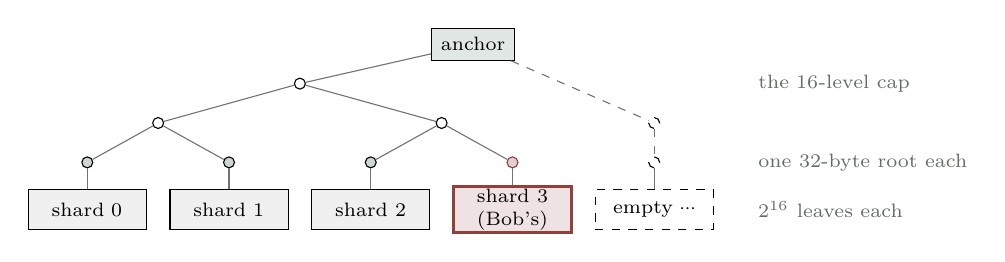
\begin{tikzpicture}[x=1mm,y=1mm,every node/.style={font=\scriptsize},
  sh/.style={draw,minimum width=15mm,minimum height=5mm,inner sep=1pt,
    align=center},
  rt/.style={draw,circle,inner sep=1.4pt},
  ed/.style={black!55}]
\node[sh,fill=black!6] (s0) at (0,0) {shard $0$};
\node[sh,fill=black!6] (s1) at (18,0) {shard $1$};
\node[sh,fill=black!6] (s2) at (36,0) {shard $2$};
\node[sh,fill=arbred!15,draw=arbred,very thick] (s3) at (54,0)
  {shard $3$\\ (Bob's)};
\node[sh,dashed] (s4) at (72,0) {empty $\cdots$};
\node[rt,fill=arb!25] (r0) at (0,6) {};
\node[rt,fill=arb!25] (r1) at (18,6) {};
\node[rt,fill=arb!25] (r2) at (36,6) {};
\node[rt,fill=arbred!25,draw=arbred] (r3) at (54,6) {};
\node[rt,dashed] (r4) at (72,6) {};
\node[rt] (a) at (9,11) {}; \node[rt] (b) at (45,11) {};
\node[rt,dashed] (c) at (72,11) {};
\node[rt] (e) at (27,16) {};
\node[draw,fill=arb!15] (R) at (49,21) {anchor};
\foreach \i in {0,...,4} {\draw[ed] (s\i) -- (r\i);}
\draw[ed] (a)--(r0); \draw[ed] (a)--(r1); \draw[ed] (b)--(r2);
\draw[ed] (b)--(r3); \draw[ed,dashed] (c)--(r4);
\draw[ed] (e)--(a); \draw[ed] (e)--(b); \draw[ed] (R)--(e);
\draw[ed,dashed] (R)--(c);
\node[anchor=west,text=arbdim] at (84,0) {$2^{16}$ leaves each};
\node[anchor=west,text=arbdim] at (84,6) {one $32$-byte root each};
\node[anchor=west,text=arbdim] at (84,16) {the $16$-level cap};
\end{tikzpicture}
\par
\begin{itemize}
  \item Cut the depth-$32$ tree at half depth: shards of $2^{16}$ leaves,
    at most $2^{16}$ of them, under a $16$-level cap of shard roots.
  \item Bob hashes his own shard from its leaves and takes every
    completed shard as one root from the server; the unfinished tip
    shard, like his own, is scanned from leaves. Low $16$ siblings from
    leaves, high $16$ from roots; an unbegun shard is a per-level
    constant.
  \item \emph{Bitcoin contrast:} an SPV client is handed one branch by
    its peer. Bob folds his own from public roots and asks for nothing
    --- asking for one note's path would say which note is his. Only
    the anchor is ever public.
\end{itemize}
\src{\emph{Ironwood Guide}, ``The wallet's witness: shardtree, shards,
  and the cap''; \emph{Wallet Guide}, ``Client state: shards, cap, and
  retention''}
\end{frame}

\begin{frame}{Checkpoints: the tree as of a block}
\begin{itemize}
  \item A \emph{checkpoint} is the wallet's record of its tree's state at
    a block boundary --- the position of the last leaf as of that block,
    plus the marks dropped since the previous one --- identified by the
    block's height.
  \item Two uses: fold a path against that block's root, so a witness
    can target any checkpointed block; and truncate the tree back to it
    when a reorganisation strikes.
  \item \emph{Shared} means present in every pool's tree: when one tree
    gains a checkpoint at a height, the others gain one too, so a single
    height names a state of every tree.
  \item A bounded recent set is kept, plus durable ones exempt from
    pruning; a block that appends nothing need not create one.
  \item \emph{Bitcoin contrast:} Bitcoin Core's checkpoints are
    hard-coded block hashes inside the node; these are wallet-local tree
    snapshots that consensus never sees.
\end{itemize}
\src{\emph{Ironwood Guide}, ``The wallet's witness: shardtree, shards,
  and the cap''; \emph{Wallet Guide}, ``Client state: shards, cap, and
  retention''; ``Reorganisation detection and recovery''}
\end{frame}

\begin{frame}{The frontier as the scan seed}
A \emph{frontier} is the rightmost path of a tree of size $n$: the last
leaf plus one sibling hash per filled subtree on its way to the root ---
enough to keep appending, and enough to seed a shard tree.
\begin{itemize}
  \item A wallet is born from the frontier of the block \emph{before} its
    birthday: that frontier summarises every earlier commitment, so no
    block below the birthday is ever replayed.
  \item Every scanned batch is seeded with the chain state of the block
    before it, checked against the first block's own end-of-block size
    before any tree is touched; a contradiction rejects the batch as
    mis-sequenced. A size the block's own contents contradict is the
    continuity error --- the reorganisation path.
  \item A found note is tree-ready once its own shard's block extent and
    the tip range are scanned --- not the whole history.
  \item \emph{Bitcoin contrast:} a restored Bitcoin wallet also rescans
    from its birthday, but needs no tree state: the UTXO set is public,
    and a peer answers a filter, or an Electrum server answers by
    address.
\end{itemize}
\src{\emph{Wallet Guide}, ``Frontiers as scan seeds''; ``The account
  birthday''; ``Shard completion and spendability''}
\end{frame}

\begin{frame}{What the server learns: the schedule}
Keys never travel; requests do. ZIP-307's stated goal is payment-detection
privacy against an honest-but-curious proxy; spending is outside its scope.
\begin{center}\small
\begin{tabular}{@{}p{0.24\textwidth}p{0.30\textwidth}p{0.38\textwidth}@{}}
\toprule
observable & reveals & mitigation status \tabularnewline
\midrule
\raggedright peer IP, connection timing &
  \raggedright endpoint, activity windows &
  \raggedright Tor capability; deployment unknown \tabularnewline
\raggedright lowest range start & \raggedright approximate account
  birthday & \raggedright none \tabularnewline
\raggedright range boundaries & \raggedright scan state and progress &
  \raggedright bucketing proposed, unimplemented \tabularnewline
\bottomrule
\end{tabular}
\end{center}
\smallskip
\emph{Bitcoin contrast:} a BIP-157 client shows a peer the same kind of
schedule --- which filter ranges it pulls, and when --- and then every
block it fetches on top. Here the content holds and the schedule leaks.
\src{\emph{Wallet Guide}, ``The stated security model''; ``What never leaves
  the device''; ``Leaks in the deployed pattern''; ``Deployed
  mitigations''}
\end{frame}

\begin{frame}{What the server learns: the content channels}
Detection stays on the device; three kinds of request carry content
anyway, each sent only after the wallet itself decided to.
\begin{center}\small
\begin{tabular}{@{}p{0.24\textwidth}p{0.30\textwidth}p{0.38\textwidth}@{}}
\toprule
observable & reveals & mitigation status \tabularnewline
\midrule
\raggedright fetch after detection &
  \raggedright\leavevmode\textcolor{arbred}{transactions of interest} &
  \raggedright decoys a SHOULD; no library policy \tabularnewline
\raggedright submission via the server &
  \raggedright the whole transaction, linked to origin &
  \raggedright circuit isolation; deployment unknown \tabularnewline
\raggedright transparent-address calls & \raggedright addresses outright &
  \raggedright jitter (one-use addresses only) \tabularnewline
\bottomrule
\end{tabular}
\end{center}
\smallskip
\emph{Bitcoin contrast:} a BIP-37 client leaks its addresses up to the
false-positive rate, a BIP-157 client its matched blocks; here content
leaks only through what the wallet sends after detecting.
\src{\emph{Wallet Guide}, ``What never leaves the device''; ``Leaks in the
  deployed pattern''; ``The submission channel''; ``Deployed
  mitigations''}
\end{frame}

\begin{frame}{Mitigations that ship, and the structural reading}
\begin{itemize}
  \item The baseline holds: across the whole service surface no request
    carries key material --- only heights, hashes, txids, transparent
    addresses, and raw transactions. Trial decryption and nullifier
    matching run on the device.
  \item Transport: a Tor client with circuit isolation exists in the
    wallet library, so submission need not share a circuit with
    scanning; whether any deployed wallet routes through it by default
    is not determinable from the sources.
  \item Timing: exponentially distributed intervals in a shuffled order
    --- only for the checks on \emph{ephemeral} addresses, the one-use
    transparent addresses of ZIP-320 payments (Part H). No jitter exists
    for the shielded fetch-on-detect.
  \item Bucketing --- rounding a range start down to a multiple of $N$
    --- is ZIP-307's own proposal, unimplemented.
  \item The reading: none of this is a property of compact-block
    contents, and none of it is inevitable; Tor, bucketing, jitter, and
    cover traffic can each change it.
\end{itemize}
\src{\emph{Wallet Guide}, ``What never leaves the device''; ``Deployed
  mitigations''; ``Summary, and the structural reading''}
\end{frame}

%% compute/f_lightclient.py:
%% tree depth 32: 32 siblings per authentication path; each root a 32-byte
%%   field element
\begin{frame}{Spending from a light client: the witness and the anchor}
\begin{itemize}
  \item Witness: Bob's $32$ siblings are folded on the device, from his
    shard's leaves and the other shards' roots, against a checkpointed
    block; the path is the private input of the membership clause.
  \item Anchor, recalled from Part C: any main-chain block's root since
    the pool's activation is admissible, no window, so proving is
    decoupled from broadcasting; appending alters no old root; an older
    anchor is no soundness hole, and a second spend is the nullifier's
    problem.
  \item \emph{Bitcoin contrast:} a Bitcoin input names one txid and index,
    and the validator looks it up. The anchor names a tree; the path into
    it never leaves the device.
\end{itemize}
\src{\emph{Ironwood Guide}, ``Anchor choice, reorgs, and the anonymity
  set''; ``The wallet's witness: shardtree, shards, and the cap''}
\end{frame}

%% compute/f_lightclient.py:
%% target = tip + 1; anchor <= target - 3 (= H - 3 with H the target);
%% confirmations: trusted 3, untrusted 10
\begin{frame}{Which anchor: the wallet's policy, and whose reasons}
\begin{itemize}
  \item Anchor: the newest shared checkpoint at or below $H - 3$, with
    $H$ the target height, one above the tip --- wallet policy, not
    consensus; ZIP-315's stated reasons and the Guide's anonymity-set
    argument are Part C's.
  \item Spendable under the same policy: $3$ confirmations for trusted
    notes, $10$ for untrusted, counted from the mined block; the note's
    shard fully scanned; and its block at or below the anchor.
  \item \emph{Bitcoin contrast:} a Bitcoin wallet also waits for
    confirmations, but which block it ``anchors'' to is nobody's
    business, because the input is named either way.
\end{itemize}
\src{\emph{Ironwood Guide}, ``Anchor choice, reorgs, and the anonymity
  set''; \emph{Wallet Guide}, ``Confirmations, trust, and spendability'';
  ``Executing the proposal''}
\end{frame}

%% compute/f_lightclient.py:
%% target = tip + 1; anchor <= target - 3 (= H - 3 with H the target);
\begin{frame}{Expiry and broadcast}
\begin{itemize}
  \item Expiry (ZIP-203): every transaction carries an expiry height,
    zero meaning none; a block that includes it above that height is
    invalid. ZIP-218 recommends target $+ 120$; a uniform delta, like a
    uniform fee, is not a fingerprint.
  \item Store, then broadcast: the wallet persists the transaction and
    locks its inputs before the network sees it, then submits it in one
    call. Once expired unmined, it releases its inputs: the notes are
    spendable again.
  \item \emph{Bitcoin contrast:} a stuck transaction has no consensus
    expiry --- mempools drop it by policy after a timeout, or RBF or CPFP
    bumps it. Here it expires by rule, and its inputs come free.
\end{itemize}
\src{\emph{Wallet Guide}, ``Expiry (ZIP-203)''; ``Store, then
  broadcast''; ``Expiry and fund availability''}
\end{frame}

\begin{frame}{The reorganisation case}
\begin{itemize}
  \item A reorganisation past the anchoring block invalidates the anchor:
    the wallet truncates to a checkpoint, rescans, and rebuilds.
  \item The rebuilt transaction re-reveals the same nullifiers, because
    their derivation is deterministic: the notes are the same, so the
    serial numbers are.
  \item Re-anchoring with the txid unchanged is specified (ZIP-374 v2,
    anchors in authorizing data); wallet support is pending.
  \item \emph{Bitcoin contrast:} a reorganised Bitcoin transaction is
    simply mined again, since it names its inputs and no anchor. Here a
    struck anchor means a rebuild.
\end{itemize}
\src{\emph{Wallet Guide}, ``Reorganisations: truncate and rescan'';
  ``PCZT v2: deferred anchors and the Ironwood bundle''}
\end{frame}

%% compute/f_lightclient.py:
%% Bob receives 1.5 ZEC; fee 10000 zatoshi; change 0.4999 ZEC to Alice's
%%   internal address
%% confirmations: trusted 3, untrusted 10
\begin{frame}{Three openings on Alice's transaction}
\begin{center}\small
\begin{tabular}{@{}llll@{}}
\toprule
ciphertext & opened by & with & yields \tabularnewline
\midrule
Action 1, \Fenc & Bob & \ivk & $(d,\ 1.5\ \text{ZEC},\ \Frseed)$; the
  memo, once fetched \tabularnewline
Action 2, \Fenc & Alice & \Fivkint & change $0.4999$ ZEC, at her internal
  address \tabularnewline
Action 1, \Fout & Alice & \ovk & $(\pkd, \esk)$, hence Bob's note as he
  reads it \tabularnewline
Action 2, \Fout & nobody & --- & random: the wallet default seals change
  under no \ovk{} \tabularnewline
\bottomrule
\end{tabular}
\end{center}
\begin{itemize}
  \item Bob: \cmx{} and \epk{} check, position recorded; with \nksym{} a
    nullifier absent from the set. From a stranger: untrusted, $10$
    confirmations.
  \item Alice finds her change by trial decryption under the internal
    scope, never through an outgoing key; internal notes are trusted:
    $3$ confirmations.
  \item Alice re-reads what she sent Bob through \Fout{} --- her sent
    history, and an auditor's, given \ovk.
  \item \emph{Bitcoin contrast:} Bob's payment and Alice's change are the
    two outputs everyone reads, and a memo would be an OP\_RETURN.
\end{itemize}
\src{\emph{Ironwood Guide}, ``Recipient: trial decryption and
  re-derivation''; ``The outgoing ciphertext''; \emph{Wallet Guide},
  ``Internal keys: change and auto-shielding''; ``Executing the
  proposal''; ``Confirmations, trust, and spendability''}
\end{frame}

%% compute/f_delivery.py:
%% compact note plaintext = 1+11+8+32 = 52 B
\begin{frame}{Checkpoint}
\Large
Bob's light client holds \ivk{} and the $52$-byte prefixes: what can the
server still infer, and what would a Bitcoin SPV client have given away
instead?
\pause
\normalsize
\bigskip
\begin{itemize}
  \item Still inferred: the endpoint and when it is active; the earliest
    range start, about his birthday; the range bounds, his progress; the
    exact txid, if he fetches the full transaction for the memo; the
    whole transaction before broadcast, if he submits through the same
    server.
  \item Never: which outputs opened, their values, or \ivk{} itself.
  \item A BIP-37 client hands each peer a Bloom filter of its scripts:
    addresses, balance, and graph, up to the false-positive rate. A
    BIP-157 client narrows that to the blocks it fetches after a match
    --- still by asking.
\end{itemize}
\src{\emph{Wallet Guide}, ``What never leaves the device''; ``Leaks in the
  deployed pattern''; ``The submission channel''}
\end{frame}

%% ---- 09-chain.tex
%% Part H --- The transaction and the turnstile (frames only).
%% Numbers: compute/h_txsize.py, h_sighash.py, h_pools.py, h_fee.py,
%% h_pczt.py, b_seal.py (outputs pasted above each frame).
\newcommand{\Hvb}{\ensuremath{v_{\mathrm{balance}}}}
\newcommand{\Hvbi}{\ensuremath{v_{\mathrm{balance}}^{\mathsf{Ironwood}}}}
\newcommand{\Hvbo}{\ensuremath{v_{\mathrm{balance}}^{\mathsf{Orchard}}}}
\newcommand{\Hd}[1]{\ensuremath{d_{\mathrm{#1}}}}

\divider{Part H}{The transaction and the turnstile}

% compute/h_txsize.py:
%   OrchardAction = 820 B; header = 20 B; signature = 64 B
%   P2PKH input = 150 B; P2PKH output = 34 B
%   proof(a) = 2720 + 2272a: a=1 -> 4992 B; a=2 -> 7264 B
%   Alice v6 (2 Ironwood Actions, all else empty) = 9166 B; proof share =
%   79.2%; sizeProofs compactSize = 3 B
\begin{frame}{A v6 transaction beside a Bitcoin transaction}
\vspace*{-4pt}
\begin{center}\small
\begin{tabular}{@{}lp{0.28\textwidth}p{0.43\textwidth}@{}}
\toprule
 & Bitcoin & Zcash v6 \\
\midrule
header & version, lock time & $+$ version group, branch id, expiry
  height: $20$~B in all \\
inputs & outpoint, scriptSig,\newline sequence & the same bytes; ECDSA over
  secp256k1, no Taproot; the scriptSig outside the txid \\
outputs & value, scriptPubKey & the same bytes \\
Sapling bundle & --- & spends, outputs, Groth16 proofs \\
Orchard bundle & --- & Actions of the sealed pool \\
Ironwood component & --- & $a$ Actions at $820$~B; flags, \Hvbi,
  anchor; one proof of $2720 + 2272a$~B; $a + 1$ signatures at $64$~B \\
\bottomrule
\end{tabular}
\end{center}
\small
One ledger, one transaction type, one asset: the shielded parts are
components beside the transparent ones. Alice's payment fills the last
component alone: $a = 2$ Actions, $7264$ proof bytes, $9166$ bytes in all.
\src{\emph{Ironwood Guide}, ``The v6 transaction and the Ironwood
  component''; \emph{Crypto Guide}, ``The transparent layer's schemes:
  ECDSA and BIP-340 over secp256k1''}
\end{frame}

% compute/h_sighash.py:
%   txid children: v5 4 (hdr, trans, Sap, Orch); v6 5 (+ Irw)
%   signature digest = txid tree with d_trans -> d_transSig; no transparent
%   inputs => identical
\begin{frame}{Effecting data, authorizing data: the SegWit shape}
\small
\begin{itemize}
  \item \textbf{Effecting data} is everything under the txid: header,
    transparent outpoints, sequences and outputs (each scriptSig is
    authorizing data: SegWit's move, applied to the legacy input), every
    Action's public fields, the flags, the balancing fields.
    \textbf{Authorizing data} is what attests to it: proofs and
    signatures --- and, from v6, the three anchors.
  \item Bitcoin's txid is SHA-256d of the bytes, and SegWit moved the
    witness out of them, re-committed through the coinbase. A v6 txid is
    a BLAKE2b-256 tree over the effecting data alone, and ZIP-244
    re-commits the authorizing data through $\mathsf{hashAuthDataRoot}$,
    folded into the header's $\mathsf{hashBlockCommitments}$. Recomputing
    a proof or a signature changes nothing the identifier names.
  \item Because the anchor is authorizing data, a v6 transaction can be
    \emph{re-anchored} --- its membership proof rebased onto a later
    root --- with its txid unchanged: specified (ZIP-374 v2), wallet
    support pending.
  \item NU7 permits v5 and v6, not v4 (draft ZIP-259).
    The Orchard-pool seal applies independently of the version.
\end{itemize}
\src{\emph{Ironwood Guide}, ``What the signatures sign: ZIP-244 digests
  and their v6 form''; ``The v6 transaction and the Ironwood component'';
  \emph{Crypto Guide}, ``The transparent layer's hashes'';
  \emph{FlyClient Guide}, ``Why an authorising-data root exists'';
  \emph{Wallet Guide}, ``PCZT v2: deferred anchors and the Ironwood
  bundle''}
\end{frame}

% compute/h_sighash.py:
%   node = BLAKE2b-256, 32 B; personalisation carries the 4-byte branch id
%   txid children: v5 4 (hdr, trans, Sap, Orch); v6 5 (+ Irw)
%   signature digest = txid tree with d_trans -> d_transSig; no transparent
%   inputs => identical
%   per-Action partition of C_enc: compact [0:52], memo [52:564], tail
%   [564:]
\begin{frame}{The sighash (ZIP-244): a tree of digests}
\begin{center}
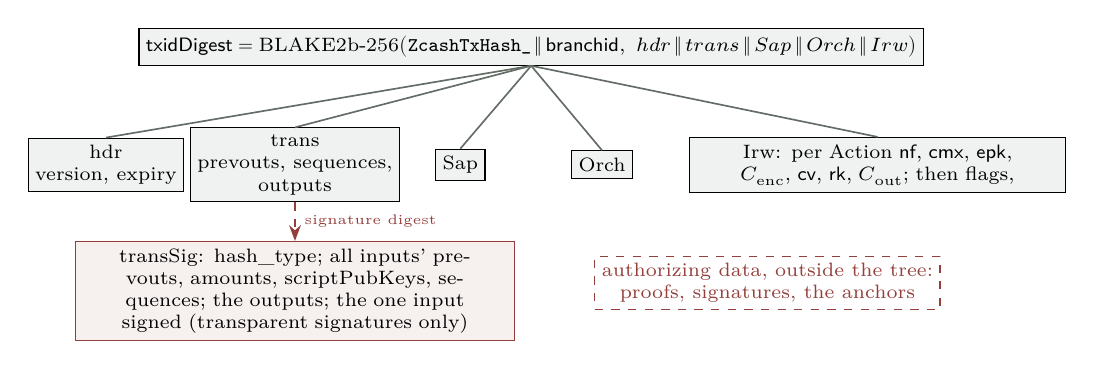
\begin{tikzpicture}[x=1mm,y=1mm,font=\scriptsize,
  nd/.style={draw,inner sep=2.5pt,align=center,fill=arb!8},
  sig/.style={draw,inner sep=2.5pt,align=center,
    fill=arbred!8,draw=arbred},
  auth/.style={draw,dashed,inner sep=2.5pt,align=center,
    draw=arbred,text=arbred},
  e/.style={-,thick,arbdim}]
\node[nd] (root) at (0,0) {$\mathsf{txidDigest} = \mathrm{BLAKE2b}%
  \text{-}256\bigl(\texttt{ZcashTxHash\_}\,\|\,\mathsf{branchid},\
  \Hd{hdr}\,\|\,\Hd{trans}\,\|\,\Hd{Sap}\,\|\,\Hd{Orch}\,\|\,\Hd{Irw}\bigr)$};
\node[nd] (hdr) at (-54,-15) {\Hd{hdr}\\version, expiry};
\node[nd] (tr) at (-30,-15) {\Hd{trans}\\prevouts, sequences,\\outputs};
\node[nd] (sap) at (-9,-15) {\Hd{Sap}};
\node[nd] (orch) at (9,-15) {\Hd{Orch}};
\node[nd,text width=46mm] (irw) at (44,-15) {\Hd{Irw}: per Action
  $\nfsym$, $\cmx$, $\epk$, $C_{\mathrm{enc}}$, $\cvsym$, $\rksym$,
  $C_{\mathrm{out}}$; then flags, \Hvbi};
\foreach \c in {hdr,tr,sap,orch,irw} \draw[e] (root.south) -- (\c.north);
\node[sig,text width=54mm] (trs) at (-30,-31) {\Hd{transSig}:
  hash\_type; all inputs' prevouts, amounts, scriptPubKeys, sequences;
  the outputs; the one input signed (transparent signatures only)};
\draw[-{Stealth[length=2mm]},arbred,dashed] (tr.south) -- (trs.north)
  node[midway,right,font=\tiny,text=arbred]{signature digest};
\node[auth] (au) at (30,-30) {authorizing data, outside the tree:\\
  proofs, signatures, the anchors};
\end{tikzpicture}
\end{center}
\small
\begin{itemize}
  \item Every node is one BLAKE2b-256 under its own personalisation; the
    root's carries the branch id, so the same bytes have a different
    identity on a parallel chain.
  \item The signature digest is this tree with \Hd{trans} swapped for
    \Hd{transSig}. A transaction with no transparent inputs has nothing
    to swap: its signature digest \emph{is} its txid.
\end{itemize}
\src{\emph{Ironwood Guide}, ``What the signatures sign: ZIP-244 digests
  and their v6 form''; \emph{Wallet Guide}, ``Serialisation and the
  transaction identifier''}
\end{frame}

% compute/h_sighash.py:
%   transparent hash_type values: 0x01, 0x02, 0x03, 0x81, 0x82, 0x83 (6;
%   ANYONECANPAY = 0x80 flag); Sapling/Orchard/Ironwood signatures:
%   SIGHASH_ALL = 0x01 always
% compute/h_fee.py: nullifiers = 2; commitments = 2 (one each per Action)
\begin{frame}{What the shielded signatures sign}
\small
\begin{itemize}
  \item Each Action's spend-authorisation signature under \rksym{} and
    the bundle's binding signature under $\mathsf{bvk}$ sign the
    signature digest: every Action's $\nfsym$, $\cmx$, $\cvsym$,
    $\rksym$ and ciphertexts, the flags, \Hvb. No Action can be
    transplanted into another transaction, no field altered.
  \item Bitcoin lets each signer pick a \texttt{hash\_type}: ALL, NONE,
    SINGLE, each with or without ANYONECANPAY --- six meaningful values
    (Taproot adds SIGHASH\_DEFAULT as a seventh spelling of ALL, which
    ZIP-244 does not define) --- and a transparent Zcash input is
    restricted by consensus to exactly those six. A shielded signature
    has one: SIGHASH\_ALL, always. There is no shielded ANYONECANPAY.
  \item The anchor is not under the signature from v6. It does not need
    to be: the proof carries it as a public input (A3), so the
    signature attests to the spend and the proof pins the tree.
  \item Alice's transaction has no transparent inputs: her two
    spend-authorisation signatures and her binding signature all sign
    her txid.
\end{itemize}
\src{\emph{Ironwood Guide}, ``What the signatures sign: ZIP-244 digests
  and their v6 form''; ``What a node verifies, without ever observing the
  note''; \emph{Wallet Guide}, ``Signing''; ``Proving''}
\end{frame}

% compute/h_pools.py:
%   fees: shielding 15000, unshielding 15000 zatoshi
%   valueBalanceIronwood: shielding -999985000 = -9.99985 ZEC;
%   unshielding +999985000 = +9.99985 ZEC
\begin{frame}{Pools and the doors}
\begin{center}
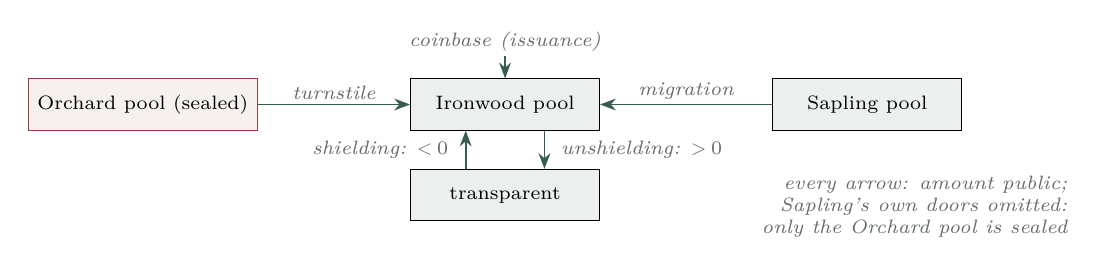
\begin{tikzpicture}[x=1mm,y=1mm,
  pool/.style={draw,minimum width=24mm,minimum height=6.5mm,
    fill=arb!10,font=\scriptsize},
  sealed/.style={pool,fill=arbred!8,draw=arbred},
  flow/.style={-{Stealth[length=2mm]},thick,arb},
  lbl/.style={font=\scriptsize\itshape,text=arbdim,inner sep=1.5pt}]
\node[sealed] (o) at (-46,0) {Orchard pool (sealed)};
\node[pool] (i) at (0,0) {Ironwood pool};
\node[pool] (s) at (46,0) {Sapling pool};
\node[pool] (t) at (0,-11.5) {transparent};
\node[lbl] (cb) at (0,8) {coinbase (issuance)};
\draw[flow] (o) -- (i) node[midway,above,lbl]{turnstile};
\draw[flow] (s) -- (i) node[midway,above,lbl]{migration};
\draw[flow] (cb) -- (i);
\draw[flow] ([xshift=-5mm]t.north) -- ([xshift=-5mm]i.south)
  node[midway,left=1.5mm,lbl]{shielding: $\Hvb < 0$};
\draw[flow] ([xshift=5mm]i.south) -- ([xshift=5mm]t.north)
  node[midway,right=1.5mm,lbl]{unshielding: $\Hvb > 0$};
\node[lbl,align=right] at (52,-13) {every arrow: amount public;\\
  Sapling's own doors omitted:\\only the Orchard pool is sealed};
\end{tikzpicture}
\end{center}
\small
\begin{itemize}
  \item \textbf{Shielding.} Transparent inputs fund a negative \Hvbi;
    the Actions spend dummies and create real notes. Alice shields
    $10$ ZEC: $\Hvbi = -9.99985$ ZEC is printed, her new note is not.
    Wallets shield automatically, to an internal address.
  \item \textbf{Coinbase.} Issuance enters a shielded pool directly, but
    every shielded coinbase output must decrypt under the all-zero
    \ovk: anyone can read what issuance entered which pool.
  \item \textbf{Migration.} Sapling or the sealed Orchard pool to
    Ironwood, the latter through the turnstile; both balancing fields
    are cleartext. Bitcoin has one pool and needs no doors.
\end{itemize}
\src{\emph{Ironwood Guide}, ``The doors: shielding, coinbase, migration'';
  ``The turnstile and migration''}
\end{frame}

% compute/h_pools.py:
%   Alice's deposit = 999985000 = 9.99985 ZEC; Bob's output = 999970000 =
%   9.9997 ZEC = 10 ZEC less two fees
%   pool balance after both, if the pool held only Alice's deposit: 0
%   zatoshi; one zatoshi more out -> -1 -> a block containing Bob's spend
%   would be invalid
\begin{frame}{The turnstile (ZIP-209): audited at the boundary}
\vspace*{-6pt}
\[
  \mathsf{balance}_{P} \;:=\; -\sum_{\mathrm{tx}} \Hvb^{P}(\mathrm{tx})
  \;\ge\; 0
  \quad\text{in every block, for }
  P \in \{\mathsf{Sap}, \mathsf{Orch}, \mathsf{Irw}\}
\]
\small
\begin{itemize}
  \item Every pool has a public balance under this rule: Sprout's is
    $\sum \mathtt{vpub\_old} - \sum \mathtt{vpub\_new}$, the transparent
    pool's the UTXO sum, the lockbox's its accrued subsidy. A block
    driving any negative, or the total past $\mathsf{MAX\_MONEY}$, is
    invalid.
  \item \emph{Inside} a pool a counterfeit is undetectable: no check sums
    the notes. Sprout's original proof system had exactly such a flaw
    (Part G); a forged proof mints silently.
  \item \emph{At the exit} the damage is capped: a forger can withdraw at
    most what the pool publicly holds. The Sapling pool still rests on
    its Groth16 ceremony; the turnstile bounds it.
  \item Had the Ironwood pool held only Alice's deposit ($9.99985$ ZEC),
    Bob's $+9.99985$ ZEC exit would empty it exactly; one zatoshi more
    and his block is invalid. Bitcoin audits by summing every coin;
    Zcash audits each pool at its door.
\end{itemize}
\src{\emph{Ironwood Guide}, ``Pool balances: ZIP-209 and its Ironwood
  analogue''; ``The turnstile and migration''; ``Prospective breaks: the
  discrete-log integrity stack''; ``Lineage: three generations of
  shielded proof''; ZIP-209; protocol specification, ``Chain Value Pool
  Balances''}
\end{frame}

% compute/b_seal.py:
%   flags byte: Orchard 0b011 (bit 2 = 0b100 clear), Ironwood 0b111 (bit 2
%   set)
\begin{frame}{Why the Orchard pool is sealed}
\small
\begin{itemize}
  \item The seal is the three rules of Parts C and E --- no issuance, no
    circulation ($\mathsf{enableCrossAddress} = 0$), no entry
    ($\Hvbo \ge 0$) --- binding whatever the transaction version.
  \item The reason is Part F's one note-level difference: a legacy note
    (lead byte $\mathtt{0x02}$) is not quantum-recoverable; an Ironwood
    note (lead byte $\mathtt{0x03}$, hashed \rcm) is. So consensus stops
    the old notes circulating and funnels their value out through the
    turnstile, while owners can still spend what they hold.
  \item The turnstile is the seal's accounting shape: the Orchard pool's
    balance can only fall, every exit metered in cleartext by \Hvbo, so
    the legacy pool drains through a public gate.
  \item Bitcoin never retires an output type; a P2PK coin spends
    forever. Here a pool can be sealed by three rules and drained
    through a metered gate.
\end{itemize}
\src{\emph{Ironwood Guide}, ``The seal: three rules''; ``One circuit,
  one verifying key''; ``ZIP-2005: quantum recoverability''; ``Pool
  balances: ZIP-209 and its Ironwood analogue''}
\end{frame}

% compute/h_fee.py:
%   Actions = 2; logical_actions = 2; fee = 5000 * max(2, 2) = 10000 zatoshi
%   one-Action shape padded to two: fee unchanged = 10000
%   shielding, 1 P2PKH input + 2 Actions: logical = 3 -> fee 15000
\begin{frame}{Fees (ZIP-317): a function of the public shape}
\begin{align*}
  \mathit{fee} &= 5000 \cdot \max(2,\ \mathit{logical\_actions})
  \quad\text{zatoshi} \\[2pt]
  \mathit{logical\_actions} &=
  \max\Bigl(\Bigl\lceil \tfrac{\text{in bytes}}{150} \Bigr\rceil,
            \Bigl\lceil \tfrac{\text{out bytes}}{34} \Bigr\rceil\Bigr)
  + 2\,\mathit{nJoinSplit}_{\mathrm{Sprout}} \\
  &\quad + \max(\mathit{spends}, \mathit{outputs})_{\mathrm{Sap}}
  + \mathit{nActions}_{\mathrm{Orch}}
  + \mathit{nActions}_{\mathrm{Irw}}
\end{align*}
\small
\begin{itemize}
  \item The divisors are the standard P2PKH input ($150$~B) and output
    ($34$~B): one typical transparent input or output weighs one action,
    and a fatter script pays in proportion.
  \item An Action spends one note \emph{and} creates one, so it is
    counted once --- charging inputs and outputs separately would tax
    the padding.
  \item Alice: two Actions, $5000 \cdot \max(2, 2) = 10\,000$ zatoshi.
    A one-Action payment padded to two pays the same. A shielding
    transaction with one P2PKH input: $1 + 2 = 3$ actions, $15\,000$.
\end{itemize}
\src{\emph{Wallet Guide}, ``The conventional fee''; ``The fee is computed
  on padded counts''}
\end{frame}

% compute/h_fee.py:
%   ZIP-317 template: block_unpaid_action_limit = 50; weight_ratio_cap = 4
\begin{frame}{Fees (ZIP-317): why a convention, and who enforces it}
\small
\begin{itemize}
  \item \textbf{Computable from public fields alone.} A fee that
    depended on which notes were spent or what change came back would
    print that data in the amount paid.
  \item \textbf{Uniform across wallets.} Every wallet is expected to pay
    exactly this fee, so the fee is not a fingerprint. Padding to two
    Actions is free by design: the grace window is two.
  \item \textbf{A convention, not consensus.} Nodes relay transactions
    paying at least it; the recommended block template picks among
    those by fee ratio, capped at $4\times$, and admits at most $50$
    unpaid actions per block. Overpaying beyond $4\times$ buys no
    further priority.
  \item \textbf{Bitcoin} runs a market: the bid per virtual byte, and
    the coin selection behind it, vary by wallet and moment --- and both
    are read as fingerprints. Zcash flattens the market on purpose.
\end{itemize}
\src{\emph{Wallet Guide}, ``The conventional fee''; ``Relay, mempool,
  and block template''}
\end{frame}

% compute/h_fee.py:
%   Actions = 2; logical_actions = 2; fee = 5000 * max(2, 2) = 10000 zatoshi
%   change = 49990000 zatoshi = 0.4999 ZEC; valueBalanceIronwood = +10000
%   zatoshi = fee
%   nullifiers = 2; commitments = 2 (one each per Action)
% compute/h_txsize.py: Alice v6 = 9166 B, proof 7264 B (79.2%)
\begin{frame}{The public face of Alice's transaction}
\begin{center}\small
\setlength{\tabcolsep}{5.5pt}
\begin{tabular}{@{}ll@{}}
\toprule
public field & Alice pays Bob $1.5$ ZEC from a $2$ ZEC note \\
\midrule
version & v6; transparent, Sapling and Orchard parts empty \\
Ironwood Actions & $2$ (one real spend, one dummy; shuffled) \\
nullifiers, commitments & $2$ and $2$ \\
\Hvbi & $+10\,000$ zatoshi $=$ the fee \\
anchor & the Ironwood root at the newest shared checkpoint at or below
  $H-3$ \\
expiry & target height $+\,120$ blocks, about $50$ minutes (ZIP-218) \\
signatures & $2$ spend-authorisation $+$ $1$ binding \\
size & $9166$ bytes, $7264$ of them proof \\
\bottomrule
\end{tabular}
\end{center}
\small
Bitcoin prints the same payment as the input coin, both amounts, both
scripts and, by subtraction, the fee. Here the fee alone is printed, as
\Hvbi; the $2$ ZEC, the $1.5$ ZEC, the $0.4999$ ZEC change and both
addresses stay inside the commitments.
\src{\emph{Ironwood Guide}, ``The v6 transaction and the Ironwood
  component''; ``Anchor choice, reorgs, and the anonymity set'';
  ``Conservation without disclosure: value commitments and the binding
  signature''; \emph{Wallet Guide}, ``Padding, dummies, and shuffling'';
  ``Expiry (ZIP-203)''}
\end{frame}

\begin{frame}{The privacy sliders: pool, address type, timing}
\small
\begin{itemize}
  \item \textbf{Pool.} A transparent leg prints its amount as \Hvb;
    fully shielded prints the fee and nothing else. The slider is the
    sender's, set by which funds and which receiver she uses.
  \item \textbf{Address type.} A unified address bundles receivers; the
    sender's wallet MUST use the most preferred one it supports:
    Orchard-protocol (into the Ironwood pool) over Sapling over
    transparent. A TEX address demands transparent funds, so the wallet
    builds two transactions through an ephemeral transparent output ---
    both public.
  \item \textbf{Timing.} ZIP-218 recommends expiry at target $+\,120$
    blocks: an idiosyncratic delta fingerprints a
    transaction as an idiosyncratic fee would. Migration wallets split
    value into canonical denominations $m \cdot 10^{k}$ ZEC,
    $m \in \{1, 2, 5\}$, and draw anchors and expiries from shared grids
    for the same reason.
  \item Bitcoin has the second and third sliders; it has no pool slider,
    because it has one plaintext ledger. Uniformity is the strategy:
    the defaults protect only while everyone keeps them.
\end{itemize}
\src{\emph{Wallet Guide}, ``Unified addresses''; ``Input selection'';
  ``Expiry (ZIP-203)''; \emph{Ironwood Guide}, ``Scheduled
  Orchard-to-Ironwood migration (ZIP-318)''}
\end{frame}

% compute/h_pczt.py:
%   ZIP-374 roles: 10 -> Creator, Constructor, IO Finalizer, Updater,
%   Prover, Signer, Combiner, Redactor, Spend Finalizer, Transaction
%   Extractor
%   PSBT roles (BIP 174/370): 7; roles PCZT adds: IO Finalizer, Prover,
%   Redactor
\begin{frame}{PSBT $\to$ PCZT (ZIP-374): the unfinished transaction}
\small
\begin{itemize}
  \item Bitcoin passes an unfinished transaction between roles --- PSBT
    (BIP-174, plus BIP-370's Constructor): Creator, Constructor, Updater,
    Signer, Combiner, Input Finalizer, Transaction Extractor --- and
    hardware wallets and multisig live on it.
  \item A PSBT cannot carry a shielded transaction: no representation
    for shielded spends and outputs, no notion of a proof distinct from
    a signature, and it tolerates unknown fields --- unacceptable for a
    signer that must understand everything it authorises.
  \item A PCZT keeps the PSBT role structure and adds Zcash's own ---
    among them an \textbf{IO Finalizer} (declares the inputs and outputs
    complete, derives the binding-signature key), a \textbf{Redactor}
    (strips what later parties need not see), and a \textbf{Prover} ---
    ten roles in all.
  \item The Prover has no PSBT counterpart because a hardware signer
    cannot compute a Halo 2 proof, and a proof needs no spending key:
    proving is delegated, signing is not. Signers can be fully offline;
    the format carries everything they need.
\end{itemize}
\src{\emph{Wallet Guide}, ``Partially created transactions (PCZT)'';
  ``Roles and lifecycle''}
\end{frame}

% compute/h_pczt.py:
%   Signer holds/needs (5): ask; alpha; rk (to check ask + alpha); sighash
%   (computed from the effecting data); the spend's public fields and,
%   unless redacted, the note fields to verify nf, cv, cmx
%   Prover needs (6): fvk; recipient, value, rho, rseed; witness; alpha;
%   rcv; anchor; no spending key
\begin{frame}{Signer versus Prover}
\begin{center}\small
\begin{tabular}{@{}lp{0.32\textwidth}p{0.38\textwidth}@{}}
\toprule
 & Signer & Prover \\
\midrule
holds & \asksym{} --- spend authority & \fvk{} --- no spending key \\
reads from the PCZT & $\alpha$, \rksym; the spend's public fields and,
  unless redacted, its note fields & the note ($\gd$, $\pkd$, $v$,
  $\rho$, $\mathsf{rseed}$), the witness, $\alpha$, \rcv, the anchor \\
computes & the sighash from the effecting data; $\rsk = \asksym +
  \alpha$, checks it matches \rksym, signs & one Halo 2 proof over all
  Actions; anchor and flags as public inputs \\
verifies first & $\nfsym$, $\cvsym$, $\cmx$ against the note fields:
  exactly what it authorises & \fvk{} owns each note;
  $\rho_{\mathrm{new}} = \nfsym_{\mathrm{old}}$ \\
learns & what it signs & the notes' private data, not authority \\
\bottomrule
\end{tabular}
\end{center}
\small
Either role can run without the other; the Prover never sees \asksym;
the Signer may see the note data, or have it redacted.
\src{\emph{Wallet Guide}, ``Signing''; ``Proving''}
\end{frame}

% compute/h_pczt.py: ZIP-374 roles: 10; roles PCZT adds: IO Finalizer,
%   Prover, Redactor
\begin{frame}{PCZT: where it stands}
\small
\begin{itemize}
  \item From v6 the Signer and the Prover are independent even of the
    anchor: signatures commit to no anchor, so a wallet can sign today
    and anchor, witness and prove at broadcast.
  \item Delegating the Prover reveals the notes' private data to the
    delegate, never spend authority; a Redactor strips what a later
    party need not see.
  \item Bins: the ZIP is Draft; the format is released as a library;
    the deployed wallet pipeline drives the roles end to end --- it
    builds the PCZT, hands it out for proving and signing, and extracts
    and stores the result (Ironwood sent-output records not yet stored:
    a backend gap, not a format limit).
  \item With FROST threshold signing (Part I) this closes the objection
    ``no script, so no multisig and no hardware wallets'': the roles
    carry both.
\end{itemize}
\src{\emph{Wallet Guide}, ``Partially created transactions (PCZT)'';
  ``Combining, redaction, and privacy''; ``The deployed wallet
  pipeline''; ``PCZT v2: deferred anchors and the Ironwood bundle''}
\end{frame}

% compute/h_pools.py:
%   fees: shielding 15000, unshielding 15000 zatoshi
%   Alice's deposit = 999985000 = 9.99985 ZEC; Bob's output = 999970000 =
%   9.9997 ZEC = 10 ZEC less two fees
%   valueBalanceIronwood: shielding -999985000 = -9.99985 ZEC;
%   unshielding +999985000 = +9.99985 ZEC
\begin{frame}{Checkpoint}
\begin{center}\large
Alice shields $10$ ZEC; the next day Bob unshields $9.9997$ ZEC.\\
What can a chain analyst conclude, and what can they not?
\end{center}
\pause
\medskip
\small
\begin{itemize}
  \item \textbf{Conclude.} Two cleartext balancing fields, exact to the
    zatoshi: $-9.99985$ ZEC entered, $+9.99985$ ZEC left --- $10$ ZEC
    less two conventional fees of $15\,000$ zatoshi; the heights; the
    transparent addresses on each side; that the amounts match exactly
    and the times are close.
  \item \textbf{Not conclude.} That Bob's coins were Alice's. Her
    commitment hides her note; his nullifier is keyed by his \nksym;
    his candidate set is every leaf under his anchor. Her note may
    still be resting.
  \item Bitcoin would have handed over the path; Zcash hands over a
    correlation. Canonical denominations and shared timing grids exist
    because that correlation is evidence.
\end{itemize}
\src{\emph{Ironwood Guide}, ``The doors: shielding, coinbase, migration'';
  ``Anchor choice, reorgs, and the anonymity set''; ``The nullifier, and
  the loop back to minting''; ``Scheduled Orchard-to-Ironwood migration
  (ZIP-318)''}
\end{frame}

%% ---- 10-consensus.tex
%% Part K --- Consensus: why one fork wins, and what the chain must remember.
%% Numbers: compute/k_catchup.py (output pasted above each frame).

%% Block tree: two panels, tied branches and their resolution.
\newcommand{\Ktree}{%
\begin{center}
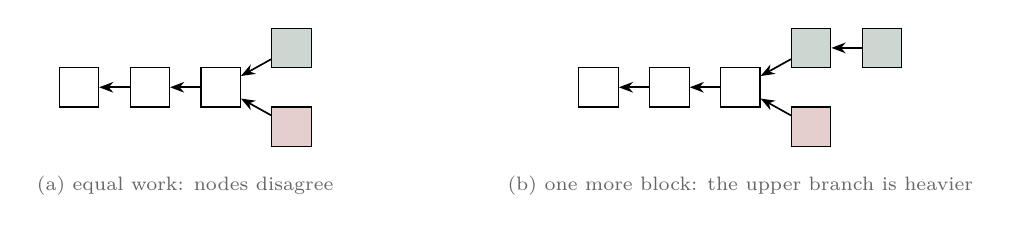
\begin{tikzpicture}[
  blk/.style={draw, rectangle, minimum width=5mm, minimum height=5mm,
    inner sep=0pt, fill=white},
  hon/.style={blk, fill=arb!25},
  att/.style={blk, fill=arbred!25},
  lnk/.style={-{Stealth[length=1.8mm]}, thick},
  lbl/.style={font=\scriptsize, text=black!60},
]
\begin{scope}
\node[blk] (g) at (0,0) {};
\node[blk] (b1) at (0.9,0) {};
\node[blk] (b2) at (1.8,0) {};
\node[hon] (c1) at (2.7,0.5) {};
\node[att] (d1) at (2.7,-0.5) {};
\draw[lnk] (b1) -- (g); \draw[lnk] (b2) -- (b1);
\draw[lnk] (c1) -- (b2); \draw[lnk] (d1) -- (b2);
\node[lbl, anchor=north] at (1.35,-1.0) {(a) equal work: nodes disagree};
\end{scope}
\begin{scope}[xshift=6.6cm]
\node[blk] (g) at (0,0) {};
\node[blk] (b1) at (0.9,0) {};
\node[blk] (b2) at (1.8,0) {};
\node[hon] (c1) at (2.7,0.5) {};
\node[hon] (c2) at (3.6,0.5) {};
\node[att] (d1) at (2.7,-0.5) {};
\draw[lnk] (b1) -- (g); \draw[lnk] (b2) -- (b1);
\draw[lnk] (c1) -- (b2); \draw[lnk] (c2) -- (c1); \draw[lnk] (d1) -- (b2);
\node[lbl, anchor=north] at (1.8,-1.0) {(b) one more block: the upper
  branch is heavier};
\end{scope}
\end{tikzpicture}
\end{center}}

%% The deficit walk: two seeded runs from z = 2 (compute/k_catchup.py).
\newcommand{\Kwalk}{%
\begin{center}
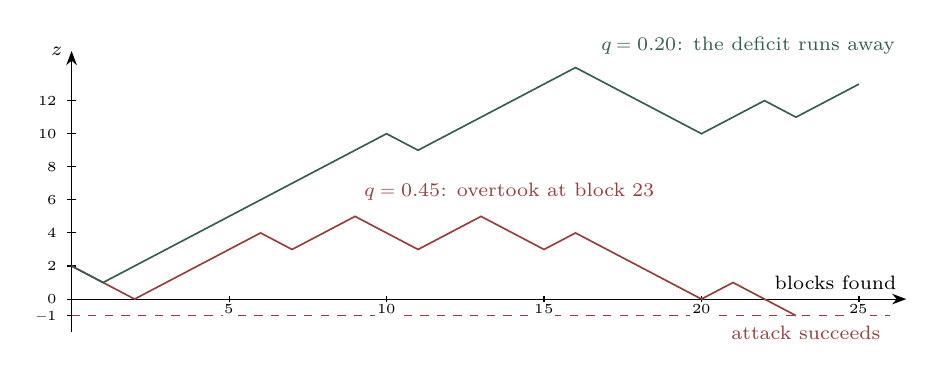
\begin{tikzpicture}[x=0.40cm, y=0.21cm]
\draw[-{Stealth[length=1.8mm]}] (0,-2) -- (0,15)
  node[left, font=\scriptsize] {$z$};
\draw[-{Stealth[length=1.8mm]}] (0,0) -- (26.5,0)
  node[above left, font=\scriptsize] {blocks found};
\foreach \y in {-1, 0, 2, 4, 6, 8, 10, 12}
  \draw (0.15,\y) -- (-0.15,\y) node[left, font=\tiny] {$\y$};
\draw[dashed, thick, arbred] (0,-1) -- (26,-1)
  node[below left, font=\scriptsize, text=arbred] {attack succeeds};
\foreach \x in {5, 10, 15, 20, 25}
  \draw (\x,0.2) -- (\x,-0.2) node[below, font=\tiny, fill=white,
    inner sep=0.6pt] {$\x$};
\draw[thick, arbred] plot coordinates {(0,2) (1,1) (2,0) (3,1) (4,2)
  (5,3) (6,4) (7,3) (8,4) (9,5) (10,4) (11,3) (12,4) (13,5) (14,4)
  (15,3) (16,4) (17,3) (18,2) (19,1) (20,0) (21,1) (22,0) (23,-1)};
\node[font=\scriptsize, text=arbred, anchor=south west] at (9,5.4)
  {$q = 0.45$: overtook at block $23$};
\draw[thick, arb] plot coordinates {(0,2) (1,1) (2,2) (3,3) (4,4) (5,5)
  (6,6) (7,7) (8,8) (9,9) (10,10) (11,9) (12,10) (13,11) (14,12) (15,13)
  (16,14) (17,13) (18,12) (19,11) (20,10) (21,11) (22,12) (23,11)
  (24,12) (25,13)};
\node[font=\scriptsize, text=arb, anchor=south west] at (16.5,14.2)
  {$q = 0.20$: the deficit runs away};
\end{tikzpicture}
\end{center}}

\divider{Part H$'$}{Consensus: why one fork wins, and what the chain must remember}

\begin{frame}{Bitcoin's chain rule, weighed in work}
\Ktree
\begin{itemize}
\item Every block names its parent, so blocks form a tree; each branch
  is one consistent history, and sibling branches may conflict.
\item The work of a block is
  $\lfloor 2^{256} / (\mathsf{ToTarget}(\mathtt{nBits}) + 1) \rfloor$;
  the best valid chain has the greatest total work; ties go to the
  block received first.
\item \alert{Bitcoin:} the same rule. ``Longest'' equals ``most work''
  only at constant difficulty, and nothing marks a chain as final --- a
  heavier branch wins however deep the fork.
\end{itemize}
\src{\emph{Consensus Guide}, ``Work, and the best chain''; protocol
  specification, ``The Block Chain''; ``Definition of Work''}
\end{frame}

\begin{frame}{Two double-spends; consensus answers one}
\begin{itemize}
\item \textbf{Same chain.} Two spends of one note reveal the same
  nullifier, and a repeated nullifier is invalid by rule (Part C, and
  later in this part). No race, no probability.
\item \textbf{Chain level.} Pay the merchant on the chain everyone
  sees, then replace that chain with one in which the payment never
  happened. No proof rules this out; only the proof-of-work race bounds
  it.
\end{itemize}
\medskip
\alert{Bitcoin:} the same two attacks; the first is a UTXO lookup there
and a nullifier lookup here.
\src{\emph{Consensus Guide}, ``Scope, sources, and the two
  double-spends''}
\end{frame}

\begin{frame}{The attack}
As Meni Rosenfeld's \emph{Analysis of hashrate-based double-spending}
--- the exact counterpart of the whitepaper's \S11, followed throughout
this part --- lays it out:
\begin{enumerate}
\item broadcast the payment to the merchant;
\item mine a secret branch from the last pre-payment block carrying a
  conflicting payment to yourself;
\item wait until the merchant ships at $n$ confirmations;
\item extend the secret branch until it carries more work, then release
  it --- a well-formed chain, merely a different one.
\end{enumerate}
\medskip
Nothing in step~4 breaks a validity rule; the only question is
probabilistic: does the secret branch ever get ahead?
\medskip

\alert{Bitcoin:} the attack the whitepaper's \S11 analyses
approximately; from here on its odds are computed exactly.
\src{\emph{Consensus Guide}, ``The attack''}
\end{frame}

% compute/k_catchup.py:
%   K2 attribution: P[next block is the attacker's] = q; independent
\begin{frame}{The model: memoryless clocks}
\begin{itemize}
\item An exponential clock of rate $\lambda$ has
  $\Pr[X > t] = e^{-\lambda t}$, and it is memoryless:
  $\Pr[X > s + t \mid X > s] = \Pr[X > t]$.
\item Two clocks race: $\Pr[X < Y] = \lambda / (\lambda + \mu)$, and
  the winner is independent of the winning time.
\item Honest network at rate $p/T_0$, attacker at $q/T_0$, $p + q = 1$,
  with $T_0$ the network's mean block time; both restart at every
  block. The next block is the attacker's with probability $q$,
  independently of everything before.
\end{itemize}
\medskip
\[
  \text{block attribution} \;=\; \text{an i.i.d. } p/q
  \text{ coin sequence};\qquad T_0 \text{ drops out of every answer.}
\]
\medskip
\alert{Bitcoin:} the whitepaper's race in Rosenfeld's model, under the
two assumptions he makes explicit --- constant hashrates and constant
difficulty. How well Equihash fits it is a deployment question (the
rails, later in this part).
\src{\emph{Consensus Guide}, ``Memoryless clocks and the attribution
  sequence''; ``Playing catch-up''}
\end{frame}

% compute/k_catchup.py:
%   K2 negative binomial, q = 1/5, n = 6: P(0)=0.262144 P(1)=0.314573
%   P(2)=0.220201 P(3)=0.117441 P(4)=0.052848 P(5)=0.021139 P(6)=0.007751
%   P(m>=6)=0.011654
\begin{frame}{The negative binomial law}
The number $m$ of attacker blocks found strictly before the honest
network's $n$-th block:
\[
  P(m) \;=\; \binom{m + n - 1}{m}\, p^{n} q^{m},
  \qquad m = 0, 1, 2, \ldots
\]
The $(m+n)$-th trial is the $n$-th honest success; the $m$ attacker
blocks sit among the first $m + n - 1$ trials in any order.
\medskip

\textbf{First-to-$n$ race.} The honest side reaches $n$ first ($H_n$)
or the attacker does ($A_n$); counts advance one at a time, so there
is no tie and $\Pr[H_n] + \Pr[A_n] = 1$.
\medskip

At $q = 1/5$, $n = 6$: $P(0) = 0.262144$, $P(1) = 0.314573$,
$P(2) = 0.220201$, \dots, $P(5) = 0.021139$;
$\Pr[m \geq 6] = 0.011654$.
\medskip

\alert{Bitcoin:} the whitepaper approximates this law by a Poisson
(the frame `Satoshi's approximation', after the worked race).
\src{\emph{Consensus Guide}, ``The negative binomial law''}
\end{frame}

% compute/k_catchup.py:
%   K3 catch-up a_z = (q/p)^(z+1), z >= 0, q < p; a_z = 1 otherwise
\begin{frame}{The catch-up theorem (Rosenfeld \S3)}
Let $z$ be the honest lead in blocks. Each block moves $z$ up by $1$
with probability $p$, down by $1$ with probability $q$. The attack
succeeds the moment $z$ reaches $-1$: strictly ahead.
\[
  a_z \;=\; \Pr[\text{walk from } z \text{ ever reaches } -1]
  \;=\;
  \begin{cases}
    1 & z < 0 \text{ or } q \geq p,\\[2pt]
    (q/p)^{\,z+1} & z \geq 0 \text{ and } q < p.
  \end{cases}
\]
\begin{itemize}
\item Each block of deficit multiplies the chance by $q/p$: two forks
  cannot compete for long, and one quickly wins.
\item At $q \geq p$ the attacker overtakes with probability $1$ from
  any finite deficit; no confirmation count defends.
\item \alert{Bitcoin:} the whitepaper writes $(q/p)^{z}$ --- it scores
  success at breakeven and banks no pre-mined block; the two
  conventions cancel term for term (shown with the confirmations).
\end{itemize}
\src{\emph{Consensus Guide}, ``Playing catch-up''}
\end{frame}

\begin{frame}{Proof idea: a walk between two barriers}
Absorb the walk at $-1$ and at $N > z$; let $h_N(z)$ be the chance of
reaching $-1$ first. Conditioning on the first step,
\[
  h_N(z) = p\, h_N(z+1) + q\, h_N(z-1), \qquad
  h_N(-1) = 1,\quad h_N(N) = 0 .
\]
The trial solution $t^{z}$ works exactly when $t$ is a root of
\[
  p\,t^{2} - t + q \;=\; p\,(t - 1)\,(t - q/p),
\]
so for $q \neq p$
\[
  h_N(z) \;=\; \frac{(q/p)^{z} - (q/p)^{N}}{(q/p)^{-1} - (q/p)^{N}}
  \;\xrightarrow{\;N \to \infty\;}\;
  \begin{cases}
    (q/p)^{\,z+1} & q < p,\\
    1 & q > p,
  \end{cases}
\]
and for $q = p$ the double root gives $h_N(z) = (N - z)/(N + 1) \to 1$.
The limit is legitimate because the events ``reach $-1$ before $N$''
increase to ``ever reach $-1$''.
\src{\emph{Consensus Guide}, ``Playing catch-up''}
\end{frame}

% compute/k_catchup.py:
%   K4 decay q=0.10: q/p=1/9, a_0=1/9=0.1111, a_1=0.0123, a_5=1.88e-06
%   K4 decay q=0.30: q/p=3/7, a_0=3/7=0.4286, a_1=0.1837, a_5=6.20e-03
%   K4 walk q=0.45 seed 0: (0,2) (1,1) (2,0) (3,1) (4,2) (5,3) (6,4) (7,3)
%   (8,4) (9,5) (10,4) (11,3) (12,4) (13,5) (14,4) (15,3) (16,4) (17,3)
%   (18,2) (19,1) (20,0) (21,1) (22,0) (23,-1)
%   K4 walk q=0.20 seed 0: (0,2) (1,1) (2,2) (3,3) (4,4) (5,5) (6,6) (7,7)
%   (8,8) (9,9) (10,10) (11,9) (12,10) (13,11) (14,12) (15,13) (16,14)
%   (17,13) (18,12) (19,11) (20,10) (21,11) (22,12) (23,11) (24,12) (25,13)
%   K4 from deficit 13 at q=0.20: a_13 = (1/4)^14 = 3.7e-09
\begin{frame}{The deficit walk}
\Kwalk
\vspace{-8pt}
Two seeded runs from $z = 2$. At $q = 0.45$ this run reaches $-1$ after
$23$ blocks; at $q = 0.20$ the deficit runs to $13$, from which the
chance of ever returning is $(1/4)^{14} \approx 3.7 \times 10^{-9}$.
Decay anchors: at $q = 10\%$, $a_0 = 1/9 \approx 0.1111$ and
$a_5 \approx 1.88 \times 10^{-6}$; at $q = 30\%$, $a_0 = 3/7 \approx
0.4286$ and $a_5 \approx 6.20 \times 10^{-3}$.
\src{\emph{Consensus Guide}, ``Playing catch-up''}
\end{frame}

% compute/k_catchup.py:
%   K5 convention z = n - m - 1
\begin{frame}{Waiting for confirmations: the pre-mined block}
The merchant ships after $n$ confirmations. Rosenfeld banks one
attacker block before the race is scored, so with $m$ further attacker
blocks the walk starts at
\[
  z \;=\; n - m - 1 .
\]
Average the catch-up probability over the negative binomial $m$:
\[
  r(q, n)
  \;=\; \underbrace{\sum_{m=0}^{n-1} P(m)\,(q/p)^{\,n-m}}_{
    \text{behind: must catch up}}
  \;+\; \underbrace{\sum_{m \geq n} P(m)}_{\text{already ahead}},
\]
and $r = 1$ when $q \geq p$, since every catch-up factor is then $1$.
The convention is a modelling choice: with no banked block the walk
starts at $n - m$ and every probability shrinks.
\medskip

\alert{Bitcoin:} this is the whitepaper's question, answered exactly
rather than approximately (next slides).
\src{\emph{Consensus Guide}, ``Waiting for confirmations''}
\end{frame}

\begin{frame}{Rosenfeld eq.~(1): the closed forms}
Each catch-up term transforms exactly,
\[
  \binom{m+n-1}{m}\, p^{n} q^{m} \left( \frac{q}{p} \right)^{\!n-m}
  \;=\; \binom{m+n-1}{m}\, p^{m} q^{n},
\]
the probability that the attacker's $n$-th block arrives while the
honest side holds $m$; summed over $m \leq n - 1$ this is $\Pr[A_n]$,
and so is the already-ahead tail. Hence
\begin{gather*}
  r(q, n)
  \;=\; 1 - \sum_{m=0}^{n-1} \binom{m+n-1}{m}
        \bigl( p^{n} q^{m} - p^{m} q^{n} \bigr) \\
  \;=\; 2 \sum_{m=0}^{n-1} \binom{m+n-1}{m} p^{m} q^{n}
  \;=\; 2 \Pr[A_n] .
\end{gather*}
\textbf{The race doubling.} Under the one-pre-mined-block convention
the catch-up half equals the already-ahead half exactly; the
double-spend probability is twice the chance of winning a first-to-$n$
race, and at $q = p$ each half is $\tfrac12$, giving $r = 1$
continuously.
\src{\emph{Consensus Guide}, ``Waiting for confirmations''}
\end{frame}

% compute/k_catchup.py:
%   K5 rows m, P(m), a_(5-m), product:
%   K5   m=0: 0.262144 0.000244 0.000064
%   K5   m=1: 0.314573 0.000977 0.000307
%   K5   m=2: 0.220201 0.003906 0.000860
%   K5   m=3: 0.117441 0.015625 0.001835
%   K5   m=4: 0.052848 0.062500 0.003303
%   K5   m=5: 0.021139 0.250000 0.005285
%   K5 catch-up half=0.011654 already-ahead half=0.011654
%   r(1/5, 6)=0.023308 = 2.3308%
\begin{frame}{A full race, exactly: $q = 1/5$, $n = 6$}
\begin{columns}[T]
\column{0.5\textwidth}
\small
\begin{tabular}{@{}rrrr@{}}
\toprule
$m$ & $P(m)$ & $a_{5-m} = 4^{-(6-m)}$ & product \\
\midrule
$0$ & $0.262144$ & $0.000244$ & $0.000064$ \\
$1$ & $0.314573$ & $0.000977$ & $0.000307$ \\
$2$ & $0.220201$ & $0.003906$ & $0.000860$ \\
$3$ & $0.117441$ & $0.015625$ & $0.001835$ \\
$4$ & $0.052848$ & $0.062500$ & $0.003303$ \\
$5$ & $0.021139$ & $0.250000$ & $0.005285$ \\
\midrule
\multicolumn{3}{@{}l}{catch-up half} & $0.011654$ \\
\multicolumn{3}{@{}l}{already-ahead half, $\Pr[m \geq 6]$} &
  $0.011654$ \\
\midrule
\multicolumn{3}{@{}l}{$r(1/5,\, 6)$} & $0.023308$ \\
\bottomrule
\end{tabular}
\column{0.46\textwidth}
\small
Every entry is an exact rational, printed to six decimals; the deficit
starts at $z = 5 - m$ and the catch-up factor is $4^{-(6-m)}$.
\medskip

The two halves agree to every digit, as the race doubling says they
must; the closed form gives the same $0.023308$.
\medskip

A merchant who ships after six confirmations against a possible
twenty-percent adversary carries a $2.33\%$ strict-overtake risk.
\medskip

\alert{Bitcoin:} six confirmations is Bitcoin's folk number; here is
what it buys, exactly.
\end{columns}
\src{\emph{Consensus Guide}, ``Waiting for confirmations''}
\end{frame}

% compute/k_catchup.py:
%   K5 Satoshi q=0.10 n=6: whitepaper 0.0243% exact 0.0591%
%   K5 Satoshi q=0.30 n=6: whitepaper 13.2111% exact 15.6450%
%   K5 Satoshi q=0.10 n=10: whitepaper 0.0001% exact 0.0008%
\begin{frame}{Satoshi's approximation}
The whitepaper computes the same quantity with one approximation and
two offsetting conventions:
\begin{itemize}
\item the attacker's progress is taken as Poisson with mean
  $\lambda = nq/p$, $\Pr[k] = e^{-\lambda} \lambda^{k} / k!$;
\item no block is pre-mined, but success is scored at breakeven rather
  than strictly ahead --- the catch-up factor is again $(q/p)^{n-m}$,
  term for term; the conventions cancel and the Poisson step is the
  entire gap.
\end{itemize}
\medskip
\begin{center}
\begin{tabular}{@{}rrrr@{}}
\toprule
$q$ & $n$ & whitepaper & exact \\
\midrule
$10\%$ & $6$ & $0.0243\%$ & $0.0591\%$ \\
$30\%$ & $6$ & $13.211\%$ & $15.645\%$ \\
$10\%$ & $10$ & $0.0001\%$ & $0.0008\%$ \\
\bottomrule
\end{tabular}
\end{center}
\medskip
In each pair the approximation understates the risk; the direction is
not uniform over all $(q, n)$. The reason to prefer the negative
binomial is that it is exact under the stated assumptions.
\src{\emph{Consensus Guide}, ``Waiting for confirmations''}
\end{frame}

% NU7 timing and risk: research/check_nu7.py.
\begin{frame}{Blocks, not time}
The catch-up formula contains neither $T_0$ nor any other time scale:
a deficit's security is a function of block \emph{counts} alone. Two
chains with the same $q$ offer identical security per confirmation ---
and therefore different security per minute.
\medskip
\begin{itemize}
\item NU7 targets $25$-second blocks; \alert{Bitcoin} $600$. Thirty
  minutes buys $3$ Bitcoin confirmations or $72$ Zcash ones in nominal
  expected time; under a $10\%$ withholding attack either wait takes
  about $33.3$ minutes, since public blocks arrive at rate $p$.
\item Conditional on those counts, at $q = 10\%$:
  $r(0.1, 3) = 1.712\%$ against $r(0.1, 72) \approx 9.35 \times
  10^{-34}$ under the model's fixed-hash-share assumption.
\item The caveat: the model has no network. Faster blocks make honest
  blocks race one another and self-orphan, which effectively raises
  $q$; the comparison holds $q$ fixed.
\end{itemize}
\src{\emph{Consensus Guide}, ``Playing catch-up''; ``Zcash time:
  25-second blocks''}
\end{frame}

% compute/k_catchup.py:
%   K6 r(q, n) percent, n = 1, 3, 6, 10:
%   K6   q= 2%: n=1:4.000 n=3:0.016 n=6:5.4e-06 n=10:1.6e-10
%   K6   q= 5%: n=1:10.000 n=3:0.232 n=6:0.0012 n=10:1.2e-06
%   K6   q=10%: n=1:20.000 n=3:1.712 n=6:0.059 n=10:0.0008
%   K6   q=20%: n=1:40.000 n=3:11.584 n=6:2.331 n=10:0.316
%   K6   q=30%: n=1:60.000 n=3:32.616 n=6:15.645 n=10:6.511
%   K6   q=40%: n=1:80.000 n=3:63.488 n=6:49.300 n=10:37.218
%   K6   q=45%: n=1:90.000 n=3:81.375 n=6:73.375 n=10:65.793
%   K6   q=50%: n=1:100.000 n=3:100.000 n=6:100.000 n=10:100.000
%   K8 wallet policy: r(0.1,3)=1.7120% r(0.1,10)=0.0008% r(0.2,10)=0.3158%
\begin{frame}{What the numbers say: $r(q, n)$ in percent}
\begin{columns}[T]
\column{0.53\textwidth}
\small
\begin{tabular}{@{}r rrrr@{}}
\toprule
$q$ & $n{=}1$ & $n{=}3$ & $n{=}6$ & $n{=}10$ \\
\midrule
$2\%$ & $4.000$ & $0.016$ & $5.4\cdot10^{-6}$ & $1.6\cdot10^{-10}$ \\
$5\%$ & $10.000$ & $0.232$ & $0.0012$ & $1.2\cdot10^{-6}$ \\
$10\%$ & $20.000$ & $1.712$ & $0.059$ & $0.0008$ \\
$20\%$ & $40.000$ & $11.584$ & $2.331$ & $0.316$ \\
$30\%$ & $60.000$ & $32.616$ & $15.645$ & $6.511$ \\
$40\%$ & $80.000$ & $63.488$ & $49.300$ & $37.218$ \\
$45\%$ & $90.000$ & $81.375$ & $73.375$ & $65.793$ \\
$50\%$ & \multicolumn{4}{c@{}}{$100$ for every $n$} \\
\bottomrule
\end{tabular}
\column{0.43\textwidth}
\small
The columns $n = 3$ and $n = 10$ are the deployed wallet defaults:
three confirmations for trusted outputs, ten for untrusted ones.
\medskip

Three confirmations assign a $10\%$ adversary $1.712\%$; ten assign the
same adversary $0.0008\%$, and a $20\%$ adversary $0.316\%$.
\medskip

Every fixed count is a $(q, \varepsilon)$ policy --- an assumed
adversary and an accepted risk --- not a law of nature.
\medskip

\alert{Bitcoin:} ``nothing is special about six'' --- it assumes an
attacker below $10\%$ and a tolerable risk below $0.1\%$; both figures
are arbitrary.
\end{columns}
\src{\emph{Consensus Guide}, ``Waiting for confirmations''; ``What the
  numbers say''; ``Wallet confirmation policy''}
\end{frame}

% compute/k_catchup.py:
%   K6 least n with r < 10%, 1%, 0.1%:
%   K6   q= 5%:   2   3   4
%   K6   q=10%:   2   4   6
%   K6   q=20%:   4   8  13
%   K6   q=30%:   9  20  32
%   K6   q=40%:  34  82 133
%   K6   q=45%: 135 331 539  (3.74 h)
\begin{frame}{Pick the adversary and the risk; read off $n$}
\begin{columns}[T]
\column{0.42\textwidth}
\small
\begin{tabular}{@{}r rrr@{}}
\toprule
$q$ & $r < 10\%$ & $r < 1\%$ & $r < 0.1\%$ \\
\midrule
$5\%$ & $2$ & $3$ & $4$ \\
$10\%$ & $2$ & $4$ & $6$ \\
$20\%$ & $4$ & $8$ & $13$ \\
$30\%$ & $9$ & $20$ & $32$ \\
$40\%$ & $34$ & $82$ & $133$ \\
$45\%$ & $135$ & $331$ & $539$ \\
\bottomrule
\end{tabular}
\column{0.54\textwidth}
\small
The least $n$ pushing $r(q, n)$ below each target: logarithmic in the
inverse risk, explosive in $q$. A $10\%$ attacker is answered by $6$
confirmations, a $45\%$ attacker by $539$ --- about $3.74$ hours of
$25$-second blocks.
\medskip

\textbf{No finite count is final:} $r(q, n) \geq 2q^{n} > 0$, since
the attacker may simply find the first $n$ blocks.
\medskip

\textbf{Divergence at the majority line:} the required $n$ tends to
infinity as $q \uparrow 1/2$, because $r(1/2, n) = 1$ for every $n$.
\medskip

\alert{Bitcoin:} the same table, the same shape; only the wall-clock
price of a row differs.
\end{columns}
\src{\emph{Consensus Guide}, ``What the numbers say''}
\end{frame}

% compute/k_catchup.py:
%   v_max = floor(o/k B (1-r)/r) = floor(4 B (1-r)/r)
\begin{frame}{The economics: when the attack pays}
The attacker targets $k$ merchants at $v$ each; the goods are worth
$\alpha v$ to him; he gives up after $o$ vain blocks; each of his
blocks would have earned the block income $B$. Expected profit over not
attacking:
\[
  k\alpha v - (1 - r)(kv + oB)
  \;=\; kv(\alpha + r - 1) - (1 - r)\,oB ,
\]
non-positive whenever
\[
  v \;\leq\; \frac{o\,(1 - r)\,B}{k\,(\alpha + r - 1)}
  \;\overset{\alpha = 1}{=}\;
  \frac{o}{k} \cdot \frac{B\,(1 - r)}{r} .
\]
\begin{itemize}
\item The cost unit $B$ is the miner's block income after the
  applicable subsidy and fee allocation. Exposure scales linearly
  with $B$; measure the payment in units of this income.
\item \alert{Bitcoin:} Rosenfeld's $B = 25$ BTC with $o = 20$, $k = 5$,
  $\alpha = 1$ gives $v \leq 100\,(1/r - 1)$ BTC; the same choices here
  give $\lfloor 4B(1 - r)/r \rfloor$.
\end{itemize}
\src{\emph{Consensus Guide}, ``The economics of the attack'';
  ``Reward-normalised exposure''; protocol specification, ``Calculating Block
  Subsidy, Funding Streams, Lockbox Disbursement, and Founders'
  Reward''; ``ZIP 214 Funding Streams''; ZIP-1016}
\end{frame}

% compute/k_catchup.py:
\begin{frame}{The largest payment the modelled attack cannot profit from}
\begin{center}
\small
\begin{tabular}{@{}r rrrrrr@{}}
\toprule
$q$ & $n{=}1$ & $2$ & $4$ & $6$ & $8$ & $10$ \\
\midrule
$5\%$ & $36$ & $271$ & $10{,}327$ & $344{,}743$ & $10{,}931{,}506$ &
  $336{,}737{,}801$ \\
$10\%$ & $16$ & $67$ & $729$ & $6{,}759$ & $59{,}475$ & $508{,}917$ \\
$20\%$ & $6$ & $15$ & $55$ & $167$ & $467$ & $1{,}262$ \\
$30\%$ & $2$ & $5$ & $11$ & $21$ & $35$ & $57$ \\
$40\%$ & $1$ & $1$ & $2$ & $4$ & $5$ & $6$ \\
\bottomrule
\end{tabular}
\end{center}
Whole block-income units: $\lfloor 4(1 - r)/r \rfloor$ ---
heuristic, as in Rosenfeld's Table~2: the unlimited-horizon $r(q, n)$
stands in for the $o = 20$ stopping rule. Against a $30\%$ attacker,
six confirmations admit $21$ whole units of $B$ under this heuristic.
Patience buys safety exponentially; the required count grows only
logarithmically in the value at stake.
\medskip

\alert{Bitcoin:} the same table with $B = 25$ BTC is Rosenfeld's
Table~2.
\src{\emph{Consensus Guide}, ``Reward-normalised exposure''}
\end{frame}

\begin{frame}{Majority is a different problem}
\begin{itemize}
\item At $q = p$ strict overtake is certain, but the walk has zero
  drift; that alone gives no lasting monopoly.
\item Past $q = p$ the attacker double-spends at no cost beyond normal
  mining, rejects every other miner's blocks to take the whole
  issuance, and excludes transactions at will --- an attempt to destroy
  the currency, motivated from outside it.
\item Confirmation policy is not the defence there; the defence is the
  cost of assembling the majority, which lies outside this model.
\end{itemize}
\medskip
\alert{Bitcoin:} Rosenfeld's remark is about Bitcoin; nothing in it
depends on the chain.
\src{\emph{Consensus Guide}, ``Reward-normalised exposure''}
\end{frame}

% compute/k_catchup.py:
%   NU7 averaging window 102, damping 4, clamps 16%/32%; Equihash (200, 9)
%   K8 r(q, 100): q=0.3:3.68e-09 q=0.4:4.32e-03 q=0.45:1.57e-01
%   K8 wallet policy: r(0.1,3)=1.7120% r(0.1,10)=0.0008% r(0.2,10)=0.3158%
\begin{frame}{NU7 rails}
\small
\begin{tabular}{@{}l p{6.3cm} p{3.6cm}@{}}
\toprule
Rail & Value & Standing \\
\midrule
Reorg window & $600$ blocks ($\approx 4.17$ h) & ZIP-218 node-policy
  recommendation \\
Coinbase maturity & $100$ blocks ($\approx 41.7$ min)
  & consensus (transparent) \\
Difficulty & every block; window $102$, damping $4$, clamp $16\%$/$32\%$
  & consensus \\
Proof of work & Equihash $(200, 9)$, SHA-256d filter & consensus \\
Wallet waits & $3$ trusted / $10$ untrusted; anchor $\leq H - 3$
  & wallet policy \\
\bottomrule
\end{tabular}
\medskip

For transparent coinbase outputs, $n = 100$: $r(0.3, 100) \approx 3.7
\times 10^{-9}$, $r(0.4, 100) \approx 0.43\%$, yet $r(0.45, 100)
\approx 15.7\%$ --- porous near the majority line, as every fixed count
must be. The window caps automatic rollback, not the theory: a fork
rooted below it needs operator intervention.
\medskip

\alert{Bitcoin:} maturity and the memoryless race are inherited;
per-block retargeting and the block spacing are not.
\src{\emph{Consensus Guide}, ``Difficulty in motion''; ``Reorg rails,
  maturity, and the finality floor''; ``Wallet confirmation policy'';
  protocol specification, ``Transaction Consensus Rules'';
  ``Difficulty adjustment''; ``Proof of Work''; draft ZIP-315}
\end{frame}

\begin{frame}{NU7: time and state}
Draft ZIPs 218 and 259; activation heights still unassigned
(23 September 2026).
\[
  \text{target spacing}:\quad 25\,\mathrm{s}
\]
\[
  \text{difficulty window}:\quad 102\cdot25 = 2550\,\mathrm{s}
\]
\[
  \text{expiry recommendation}:\quad
  120\cdot25 = 3000\,\mathrm{s}
\]
\medskip
No new transaction format: v5 and v6 remain; v4 is rejected.
ZIP-237 adds delayed reissuance of funds removed from circulation
to the halving-based subsidy.
\src{\href{https://github.com/zcash/zips/pull/1363}{ZIP-259};
  \href{https://zips.z.cash/zip-0218}{ZIP-218};
  \href{https://github.com/zcash/zips/pull/1354}{ZIP-237}}
\end{frame}

\begin{frame}{Where the deployed rule departs from the model}
\begin{itemize}
\item \textbf{The tie-break.} The specification and Rosenfeld break
  equal-work ties first-seen. Zebra downloads blocks in parallel and
  tracks no arrival times, so it prefers the larger tip hash --- its
  own documentation calls this a departure from the consensus rules.
\item \textbf{What that does to $r$.} At equal work an attacker whose
  private tip hash wins may reveal at once; the strict-overtake
  boundary $z = -1$ does not count that success. So $r(q, n)$ is exact
  for the strict-overtake model and a lower bound if only the tie-break
  is replaced by Zebra's --- not a bound on the full deployed process,
  where difficulty moves and rollback is capped.
\item \textbf{Equihash and memorylessness.} Each candidate solution
  faces a fresh SHA-256d lottery, so headers are the Bernoulli trials
  of the model; what Equihash changes is granularity --- candidates
  arrive per solver run, and the exponential clock is good only while
  a run is short against the NU7 target spacing of $25$ seconds.
\end{itemize}
\alert{Bitcoin:} its nodes keep the first-seen rule; its hash trials
are the model's ideal.
\src{\emph{Consensus Guide}, ``Chain selection and the tie-break''; ``Equihash
  and the memoryless model''}
\end{frame}

\begin{frame}{What consensus adds for shielded state: the nullifier set}
The specification's rule, verbatim: ``A nullifier MUST NOT repeat
either within a transaction, or across transactions in a valid block
chain.'' Each pool's nullifiers are ``considered disjoint, even if they
have the same bit pattern''.
\medskip
\begin{itemize}
\item The check is \emph{stateful and ordered}: transactions apply in
  block order; each $\nfsym_{\mathrm{old}}$ is tested against the set
  as it stands, then recorded, then each $\cmx_{\mathrm{new}}$ is
  appended. The next spender proves membership against the new root;
  a second spend of the same note fails.
\item It is the one check that cannot sit inside a proof, because it
  concerns the global history, not one transaction.
\item Sets are per pool (ZIP-229): uniqueness of $\rho_{\mathrm{new}}
  := \nfsym_{\mathrm{old}}$ is pool-local, not global.
\end{itemize}
\medskip
\alert{Bitcoin:} the UTXO set is the same kind of ordered stateful
check; here the set records serial numbers that name no output.
\src{protocol specification, ``Nullifier Sets''; \emph{Ironwood Guide},
  ``What a node verifies, without ever observing the note''; ``The
  nullifier, and the loop back to minting''}
\end{frame}

\begin{frame}{Anchors, balances, and no mempool chains}
\begin{itemize}
\item \textbf{Anchors.} The bundle's anchor ``MUST refer to some
  earlier block's final'' treestate for its pool --- never a mid-block
  state, and any main-chain block since the pool's activation
  qualifies; the depth $H - 3$ is wallet policy.
\item \textbf{No spend of an unmined note.} An Action cannot spend an
  output of its own transaction, and a note mined in this block is
  under no earlier block's final root. \alert{Bitcoin} lets a mempool
  chain spend unconfirmed outputs; a shielded note cannot be spent
  until it is mined (the transparent layer keeps Bitcoin's rule).
\item \textbf{The specified route.} ZIP-374 makes v6 anchors
  deferrable: sign a spend of a not-yet-mined note now, fill the anchor
  after the note is mined; signatures commit to neither anchor nor
  witness.
\item \textbf{Balances.} Each pool's chain value balance is public and
  a block that would drive one negative is invalid (ZIP-209);
  every crossing writes a public row.
\end{itemize}
\src{protocol specification, ``Transactions and Treestates'';
  ``Action Transfers and their Descriptions''; \emph{Ironwood Guide},
  ``Anchor choice, reorgs, and the anonymity set''; ``Pool balances:
  ZIP-209 and its Ironwood analogue'';
  \emph{Wallet Guide}, ``PCZT v2: deferred anchors and the Ironwood
  bundle''}
\end{frame}

\begin{frame}{Reorganisation of shielded state}
\begin{itemize}
\item Trees, nullifier sets, and pool balances are chain state; a
  reorganisation rolls all three back together with the blocks.
\item A reorganisation reaching the anchoring block strikes the anchor
  and the transaction with it. The rebuild spends the same notes, and
  nullifier derivation is deterministic, so it re-reveals the same
  nullifiers (the rebuild, truncate-and-rescan, and ZIP-374's
  re-anchoring: Part C).
\end{itemize}
\medskip
\alert{Bitcoin:} a transaction struck by a reorganisation is simply
re-broadcast unchanged; here, once the fork reaches the anchoring
block, the proof must be rebuilt against a surviving root.
\src{\emph{Ironwood Guide}, ``Anchor choice, reorgs, and the anonymity
  set''; \emph{Wallet Guide}, ``Reorganisations: truncate and rescan'';
  protocol specification, ``Transactions and Treestates''}
\end{frame}

% compute/k_catchup.py:
%   K6   q=20%: n=1:40.000 n=3:11.584 n=6:2.331 n=10:0.316
%   K8 wallet policy: r(0.1,3)=1.7120% r(0.1,10)=0.0008% r(0.2,10)=0.3158%
\begin{frame}{Checkpoint}
A merchant sees Alice's shielded payment at one confirmation. Which of
the two double-spends is she exposed to, and what does the catch-up
theorem say about waiting?
\pause
\medskip

\begin{itemize}
\item Not the same-chain one: a second spend of Alice's note reveals
  the same nullifier, and the set rejects it by rule, at any depth.
\item The chain-level one: a secret branch may replace the block she
  saw. At $n = 1$ a $20\%$ adversary succeeds in $40\%$ of runs; each
  added confirmation drops the risk by a roughly constant factor, and
  $r(0.2, 10) = 0.316\%$.
\item Waiting works in blocks, not minutes; it never reaches zero, and
  it stops working at $q = 1/2$.
\end{itemize}
\src{\emph{Consensus Guide}, ``Playing catch-up''; ``What the numbers
  say''; protocol specification, ``Nullifier Sets''}
\end{frame}

%% ---- 11-close.tex
%% Part I --- Limits, frontier, takeaways

\divider{Part I}{Limits, frontier, takeaways}

% compute/ep_actions.py:
%   Actions: 2 (requested spends 1, outputs 2, padded to MIN_ACTIONS = 2)
%   fee = 5000 * max(2, 2) = 10000 zatoshi
%   amounts: in 200000000 -> Bob 150000000, change 49990000 zatoshi (0.4999 ZEC)
%   valueBalance = +10000 zatoshi = fee
%   per-Action sums: +50000000 and -49990000 -> 10000
%   bytes: Actions 820 * 2 = 1640; proof 2720 + 2272 * 2 = 7264;
%     SpendAuthSigs 64 * 2 = 128; binding sig 64; signatures 128 + 64 = 192
%   public per Action: nf, cmx, cv, rk, epk, C_enc, C_out -> 2 nullifiers,
%     2 commitments
\begin{frame}{Limits: what the theorem leaves public}
The end-to-end theorem hides the note contents and the spend-to-note
link. It does not claim to hide:
\begin{itemize}
  \item the public balance, the component and Action counts, any
    transparent leg, timing, address reuse, voluntary disclosures,
    wallet and network metadata;
  \item on Alice's bundle: two Actions, one anchor, two nullifiers, two
    commitments, and $\mathrm{valueBalance} = +10\,000$ zatoshi --- the
    fee, in the clear.
\end{itemize}
The candidate set is the tree under the anchor, but publicly known dummy
or spent leaves and other transaction metadata reduce the effective
anonymity set; tree size alone does not measure it. An idiosyncratically
old anchor fingerprints the spender.

\medskip
\alert{Bitcoin:} the graph itself is published. Here the graph is gone
and the envelope stays: counts, fee, anchor, timing.
\src{\emph{Ironwood Guide}, ``Composition: the end-to-end theorem'';
``Resting: the note in the commitment tree''; ``Anchor choice, reorgs,
and the anonymity set''}
\end{frame}

\begin{frame}{Limits: the light client's server}
The stated goal (ZIP-307): an honest-but-curious server must not learn
which transactions are a wallet's. The keys never travel; the requests do
--- the full inventory is \emph{Delivery and light clients}, ``What the
server learns''. Two leaks survive the shipped mitigations:
\begin{itemize}
  \item \textbf{Fetch-on-detect names a txid.} A scan is issued with exact
    range bounds and no per-block match; the full transaction fetched
    after a hit (the memo is not in the compact block) names exactly one
    transaction. The decoy fetches ZIP-307 asks for are a SHOULD the
    reference library does not supply.
  \item \textbf{The submission channel links the transaction to its
    origin.} A wallet that broadcasts through the same server hands it
    the whole transaction before the network sees it, tied to the session
    that scanned; circuit isolation exists in the client library, its
    deployment unknown.
\end{itemize}
\alert{Bitcoin:} the scan leaks less than a BIP-157 client, which names
each block it fetches after a filter hit; the fetch after a hit leaks
more --- one txid, not a block (``Leaks, in both directions'').
\src{\emph{Wallet Guide}, ``The stated security model''; ``Leaks in the
deployed pattern''; ``The submission channel''; ``Deployed mitigations''}
\end{frame}

% compute/d_keys.py:
%   seed: 32..252 bytes, >= 256 bits entropy; sk 32 bytes = 256 bits
%   diversifier 88 bits; addresses per account per scope 2^88
\begin{frame}{Limits: custody is a key}
A note is $(\mathsf{addr}, v, \rho, \psi, \rcm)$: it carries no script.
Its spending condition is knowledge of \asksym, proved through \rksym{}
(A6, A7) --- whoever holds \asksym{} spends, and nothing below it on the
ladder recovers it.
\begin{itemize}
  \item Every key descends from one seed $S$: $32$ to $252$ bytes, at
    least $256$ bits of entropy (ZIP-32). A weak seed is a weak link for
    all of them at once, and a brute-force search over weak seeds runs
    against many wallets simultaneously.
  \item What script gave Bitcoin moves into the wallet layer: threshold
    authority is FROST ($t$-of-$n$ over \asksym; the verifier is
    untouched); hardware and offline signers use PCZT (a signer holds
    \asksym{} but cannot compute a Halo 2 proof).
\end{itemize}
\alert{Bitcoin:} spending conditions live in script and every validator
runs them --- multisig, timelocks, hash locks. Here the condition is
fixed by the circuit and discharged by one signature.
\src{\emph{Ironwood Guide}, ``The note and its commitment''; ``The
capability ladder''; \emph{Wallet Guide}, ``Wallet seeds''; ``Partially
created transactions (PCZT)''; \emph{FROST Guide}, ``Scope''}
\end{frame}

\begin{frame}{Quantum: two kinds of break}
A CRQC --- a quantum computer running Shor's algorithm at scale --- takes
discrete logarithms in polynomial time; every group assumption falls.
\begin{center}
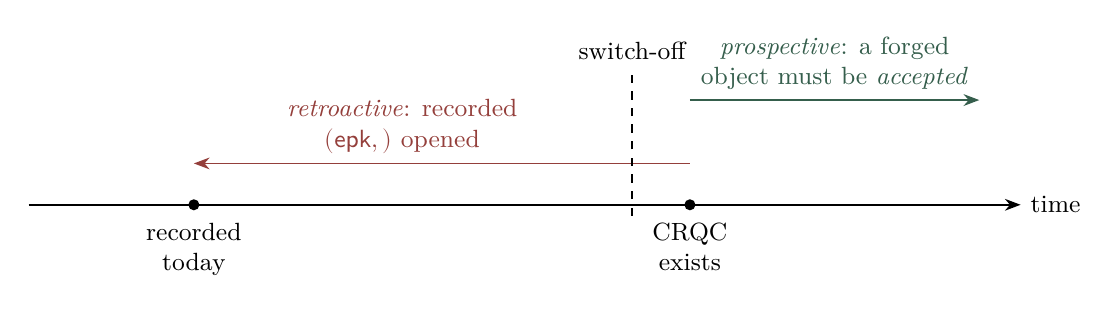
\begin{tikzpicture}[x=1.05cm, y=0.7cm, >={Stealth[length=2mm]},
  lab/.style={font=\small, align=center}]
\draw[->, thick] (0,0) -- (12,0) node[right, font=\small] {time};
\fill (2,0) circle (2pt);
\node[lab, below=3pt] at (2,0) {recorded\\today};
\fill (8,0) circle (2pt);
\node[lab, below=3pt] at (8,0) {CRQC\\exists};
\draw[<-, thick, arbred] (2,0.75) -- (8,0.75)
  node[pos=0.42, above, lab] {\emph{retroactive}: recorded\\
  $(\epk, \Cenc)$ opened};
\draw[->, thick, arb] (8,1.9) -- (11.5,1.9)
  node[midway, above, lab] {\emph{prospective}: a forged\\object must
  be \emph{accepted}};
\draw[dashed, thick] (7.3,-0.2) -- (7.3,2.45) node[above, font=\small]
  {switch-off};
\end{tikzpicture}
\end{center}
Retroactive: recorded data is exploitable the day the adversary exists.
Prospective: a validator must \emph{accept} a forgery, so switching off
first removes acceptance. Orchard, both pools: one retroactive break.

\alert{Bitcoin:} no ciphertext to open, but a silent-payment scan key has
the same retroactive shape (next frame); an exposed public key is the
prospective case.
\src{\emph{Ironwood Guide}, ``The reversibility taxonomy and the
epistemic bins''; \emph{Crypto Guide}, ``The quantum caveat: Shor's
algorithm''}
\end{frame}

\begin{frame}{Retroactive: harvest now, decrypt later}
Each Action publishes $(\epk, \Cenc)$; one discrete-log link
protects it, the Diffie--Hellman between \esk{} and \pkd{} --- the KDF
and AEAD above it are symmetric.
\[
\ivk = \log_{\gd}\pkd
\quad\Longrightarrow\quad
K = \mathrm{KDF}\bigl([\ivk]\,\epk, \ldots\bigr)
\]
One logarithm for the lifetime of the \ivk{} scope, then the recipient's
own trial-decryption loop over the recorded chain: every $(d, v,
\mathsf{rseed}, \mathsf{memo})$ ever sent to any diversified address
sharing that \ivk, past and future.

\medskip
Bob's address went to Alice; whoever else holds it can one day read the
$1.5$ ZEC and the memo.
\src{\emph{Ironwood Guide}, ``The retroactive break: harvest now, decrypt
later''}
\end{frame}

\begin{frame}{Retroactive: two limits, and the bin}
\begin{itemize}
  \item \ivk{} views and never spends: no spend authority is conferred,
    and \asksym{} is not exposed --- its exposure is the prospective case.
  \item The attack is keyed by the address: without $(d, \pkd)$ there is
    neither the base \gd{} nor the target \pkd, and no known efficient
    generic route exists from the ciphertext alone.
  \item Bin: \emph{open problem}. Nothing deployed or specified protects
    even future ciphertexts (ZIP-2005 excludes privacy by an explicit
    non-requirement); the recorded ones are unrepairable.
\end{itemize}
\alert{Bitcoin:} no ciphertext to open, but silent payments carry the same
shape: one logarithm of the published scan key replays the recipient's
scan over recorded history and links everything that address ever
received. No analogue for the amount and the memo --- Bitcoin never hid
them.
\src{\emph{Ironwood Guide}, ``The retroactive break: harvest now, decrypt
later''; ZIP-2005, ``Non-requirements''}
\end{frame}

\begin{frame}{Prospective: the discrete-log integrity stack}
Shor invalidates the reductions; each construction gets its own concrete
consequence.
\begin{center}\small
\begin{tabular}{@{}p{0.24\textwidth}p{0.70\textwidth}@{}}
\toprule
construction & with the generators' logarithms known \\
\midrule
\raggedright Sinsemilla binding (\NoteCommit, \CommitIvk) & a second note
  under an on-chain \cmx{} --- balance breaks silently,
  turnstile-bounded; a second $(\aksym, \nksym)$ for the same \ivk{} ---
  a spendability forgery \\
\raggedright value commitment, binding signature & any \cvsym{} reopens to any
  value; a solved $\mathsf{bvk}$ forges the signature --- inflation,
  turnstile-bounded \\
\raggedright spend authorisation (RedPallas) & one logarithm of \aksym{} or
  of any
  published \rksym{} forges spend authority; theft still needs a
  witness or a proof forgery \\
\raggedright proof soundness (IPA on Vesta) & commitment equivocation; the
  knowledge-soundness reduction no longer holds \\
\bottomrule
\end{tabular}
\end{center}
Recorded \cvsym{} values stay perfectly hiding; $\alpha$ masks \rksym;
transcripts are simulatable. Without the address, no generic route pulls
these secrets from the recorded fields.
\src{\emph{Ironwood Guide}, ``Prospective breaks: the discrete-log
integrity stack''}
\end{frame}

\begin{frame}{Why the integrity breaks are prospective}
Each attack must place a forged object --- a proof, a signature, a
commitment opening --- before a validator and have it \emph{accepted},
at current height under current rules.
\begin{itemize}
  \item Disabling the discrete-log pools before a CRQC exists removes
    acceptance of new transactions under those rules; settled history
    stays anchored by chain work and upgrade policy.
  \item Residue one: switch-off must precede the \emph{first} forgery ---
    an attack landed inside the window is not repaired afterwards.
  \item Residue two: honest funds inside a disabled pool need another way
    out. That is the problem ZIP-2005 exists to solve.
\end{itemize}
\alert{Bitcoin:} the same shape. ECDSA and Schnorr fall to one logarithm
of an exposed public key, and the forged spend must still be mined.
\src{\emph{Ironwood Guide}, ``Prospective breaks: the discrete-log
integrity stack''; \emph{Crypto Guide}, ``The quantum caveat: Shor's
algorithm''}
\end{frame}

% compute/i_limits.py:
%   grover: 2^256 classical preimage evaluations -> ~2^128 quantum
%   bht collision: 2^(n/3) = 2^85 queries (needs ~2^92 bits of QRAM; not
%   the slide's number)
\begin{frame}{The symmetric backbone survives}
Two primitive families carry no discrete-log structure.
\begin{itemize}
  \item BLAKE2b: $\mathsf{PRFexpand}$, hence every key and note-randomness
    derivation, the KDF, the outgoing cipher key, the RedPallas challenge,
    the ZIP-244 digests; the ZIP-32 Orchard tree is hardened-only and
    built entirely from it.
  \item Poseidon: the nullifier PRF, keyed by \nksym{} --- a
    cryptanalytic heuristic, classically and quantumly alike.
\end{itemize}
Generic speedups only: Grover halves preimage security,
\[
2^{256} \text{ classical evaluations} \;\longrightarrow\; \approx 2^{128}
\text{ quantum ones,}
\]
and the best implementable generic collision attack remains the
classical parallel one. The load-bearing consequence: a seed holder can
still prove, by re-executing the hardened derivations, that their keys
descend from their seed. Ownership stays \emph{provable} after the
assumption that made it \emph{enforceable} has fallen.

\alert{Bitcoin:} SHA-256 and hardened BIP-32 derivation stand on the same
ground.
\src{\emph{Ironwood Guide}, ``Primitives facing only generic speedups'';
\emph{Crypto Guide}, ``The quantum caveat: Shor's algorithm''}
\end{frame}

% compute/b_quantum.py:
%   log2 N = log2 p_Vesta = 254.0000
%   q = 2^60: log2(q^3/N) = -74.0; log2(q^2/N) = -134.0
%   pre_rcm = 1+32+32+8+32+32 = 137 bytes
%   Recovery Statement cost: 7 BLAKE2b-512 compressions, 1 BLAKE3
%     compression, 2 Sinsemilla commitments, 2 Pallas scalar
%     multiplications, 1 Merkle path
\begin{frame}{ZIP-2005: the hashed trapdoor}
Recall the one note-level difference between the pools (``The Ironwood
trapdoor''):
\[
\rcm := \mathrm{ToScalar}\bigl(\mathsf{PRFexpand}_{\mathsf{rseed}}(
\mathtt{0x0B} \,\|\, \gd^\star \,\|\, \pkd^\star \,\|\, \mathrm{LE}_{64}(v)
\,\|\, \mathrm{LE}_{256}(\rho) \,\|\, \mathrm{LE}_{256}(\psi))\bigr),
\]
a $137$-byte preimage: every note field traverses BLAKE2b into the
trapdoor.
\begin{itemize}
  \item Under a CRQC, \NoteCommit{} alone is not binding --- Sinsemilla's
    collision resistance is the first thing to fall.
  \item Model $\mathsf{PRFexpand}$ as a random oracle: opening one
    commitment to two honestly derived notes is a collision-type event,
    with no group structure for Shor. Bound $O(q^3/N)$ in the QROM, about
    $2^{-74}$ at $q = 2^{60}$.
  \item The composite is post-quantum binding \emph{provided a verifier
    checks the derivation}. No deployed clause does --- that check is the
    Recovery Statement's job.
  \item Legacy $\mathtt{0x02}$ notes hash $\mathtt{0x05} \,\|\, \rho$
    only: unrecoverable, hence the seal (``Why the Orchard pool is
    sealed'').
\end{itemize}
\alert{Bitcoin:} ownership is a public key, exposed at spend; the hardened
derivation behind it is symmetric too, but no rule reads it --- the
exposed key alone decides a spend.
\src{\emph{Ironwood Guide}, ``The note seed: Ironwood derivations (lead
byte $\mathtt{0x03}$)''; ``ZIP-2005: quantum recoverability''; ``The
seal: three rules''}
\end{frame}

% compute/b_quantum.py:
%   Recovery Statement cost: 7 BLAKE2b-512 compressions, 1 BLAKE3
%     compression, 2 Sinsemilla commitments, 2 Pallas scalar
%     multiplications, 1 Merkle path
\begin{frame}{Recoverability, not resistance}
The Recovery Statement, proved one day in a post-quantum proof system
over a re-hashed tree: the key derivations from $\mathsf{sk}$, $\ivk =
\CommitIvk$, $\pkd = [\ivk]\,\gd$, the $\psi$ and \rcm{} derivations,
the commitment, a membership path, the nullifier, the $\alpha$
re-randomisation. Cost: $7$ BLAKE2b-512 compressions, $1$ BLAKE3
compression, $2$ Sinsemilla commitments, $2$ Pallas scalar
multiplications, a Merkle path.

\medskip
Binding only, privacy unchanged: the statement proves, with no group
assumption, that one seed derives a committed note, its nullifier and its
\rksym; it opens no ciphertext.
\src{\emph{Ironwood Guide}, ``ZIP-2005: quantum recoverability'';
``Strategy: recoverability, not resistance''}
\end{frame}

\begin{frame}{ZIP-2005: deployed, specified, designed, open}
\begin{itemize}
  \item \emph{Specified and deployed}: the $\mathtt{0x03}$ derivation and
    the three seal rules --- every Ironwood output is recoverable.
  \item \emph{Specified, undeployed}: the quantum-key path
    ($\mathsf{qsk}$, $\mathsf{qk}$); no consensus rule.
  \item \emph{Designed, unspecified}: the Recovery Protocol --- proof
    system, collapsing tree hash, linking commitments all unfixed.
  \item \emph{Open}: post-quantum proofs and signatures for ongoing
    spends; the switch-off schedule.
\end{itemize}
Sprout, Sapling and Orchard-pool notes are unrecoverable, so ZIP-2005
tells wallets to sweep everything into Ironwood as an ongoing process;
deployed today, change is routed there. The one cost the strategy cannot
answer: the harvested corpus accrues now.
\src{\emph{Ironwood Guide}, ``ZIP-2005: quantum recoverability'';
``Strategy: recoverability, not resistance''; ``Change and wallet
posture''}
\end{frame}

\begin{frame}{Beyond the core: what each one adds}
\begin{center}\small
\begin{tabular}{@{}p{0.10\textwidth}p{0.50\textwidth}p{0.30\textwidth}@{}}
\toprule
 & what it adds & Bitcoin \\
\midrule
FROST & \raggedright $t$-of-$n$ custody of \asksym; the aggregate is an
  ordinary spend-auth signature under \rksym & a Taproot FROST suite \\
\addlinespace
FlyClient & \raggedright logarithmic chain proofs: difficulty-weighted
  sampling over a Merkle mountain range & SPV fetches every header \\
\addlinespace
ZSA & \raggedright issued assets: per-asset notes and value commitments,
  issuance, burn & Elements' issued assets \\
\addlinespace
Crosslink & \raggedright proof of work kept, plus a trailing BFT finality
  layer cross-linked with it & confirmations, never finality \\
\bottomrule
\end{tabular}
\end{center}
None of the four adds privacy: they add custody, chain verification,
assets, and settlement to a core whose hiding is unchanged.
\src{\emph{FROST Guide}, ``Scope''; \emph{FlyClient Guide}, ``The
deployment boundary, stated at the outset''; ``The cost of header-only
verification''; \emph{ZSA Guide}, ``Method: the three bins for ZSA'';
\emph{Crosslink Guide}, ``Scope, status, and sources''}
\end{frame}

\begin{frame}{Beyond the core: the bins}
\begin{center}\small
\begin{tabular}{@{}p{0.10\textwidth}p{0.84\textwidth}@{}}
\toprule
 & bin, as the volume states it \\
\midrule
FROST & \emph{specified}: RFC 9591 and ZIP-312 (Draft); shipped as a
  library; no consensus rule names it; key generation in no ZIP \\
\addlinespace
FlyClient & commitment \emph{deployed and consensus-critical} (ZIP-221,
  its root committed in every header since Heartwood); proofs
  \emph{unbuilt}: no server serves one, no client asks; the Zcash
  instantiation designed, not specified \\
\addlinespace
ZSA & core \emph{specified} in Draft ZIPs 226 and 227; the carrier ---
  v6 wire format, digests, lead byte, fees --- \emph{unspecified} since
  the ZIPs that held it were withdrawn; outside ZIP-259's NU7 scope \\
\addlinespace
Crosslink & \emph{design stage}: no ZIP, nothing activated on mainnet or
  testnet; a feature net runs prototype code; the construction rules
  \emph{designed but unspecified} \\
\bottomrule
\end{tabular}
\end{center}
Three bins throughout the volumes: \emph{specified}, \emph{designed but
unspecified}, \emph{open problem}; deployed behaviour cites the
implementation and the specification instead.
\src{\emph{FROST Guide}, ``The three-bin rule''; \emph{FlyClient Guide},
``The deployment boundary, stated at the outset''; ``The light-client
stack consumes none of it''; \emph{ZSA Guide}, ``Status''; ``Method: the
three bins for ZSA''; \emph{Crosslink Guide}, ``The three bins, and a
proved tag''; ``Scope, status, and sources''}
\end{frame}

\begin{frame}{Where each one sits}
\begin{center}
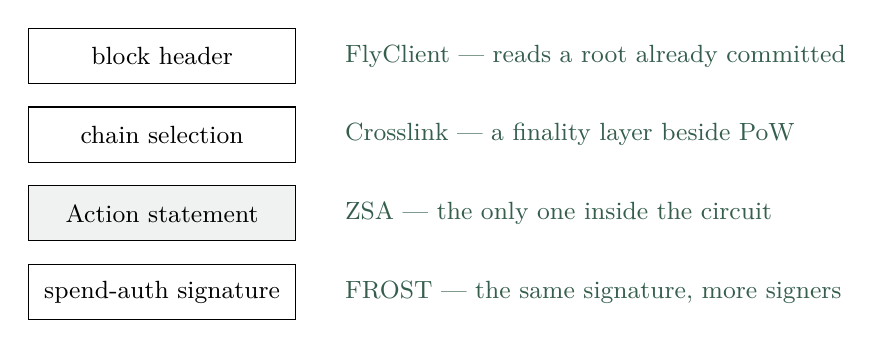
\begin{tikzpicture}[x=1cm, y=1cm, >={Stealth[length=2mm]},
  layer/.style={draw, minimum height=7mm,
    minimum width=34mm, font=\small, align=center},
  tag/.style={font=\small, text=arb, anchor=west}]
\node[layer] (hdr) at (0,3.0) {block header};
\node[layer] (cons) at (0,2.0) {chain selection};
\node[layer, fill=arb!8] (stmt) at (0,1.0) {Action statement};
\node[layer] (sig) at (0,0) {spend-auth signature};
\node[tag] at (2.2,3.0) {FlyClient --- reads a root already committed};
\node[tag] at (2.2,2.0) {Crosslink --- a finality layer beside PoW};
\node[tag] at (2.2,1.0) {ZSA --- the only one inside the circuit};
\node[tag] at (2.2,0) {FROST --- the same signature, more signers};
\end{tikzpicture}
\end{center}
Only ZSA changes the statement: an Asset Base witnessed once, A1 and A2
on a per-asset commitment, A4 by variable-base multiplication, the A3
dummy skip kept for the native asset alone, split notes. The other three
leave the ten clauses as they are.
\src{\emph{ZSA Guide}, ``The Action statement, extended''; \emph{FROST
Guide}, ``Scope''; \emph{FlyClient Guide}, ``The deployment boundary,
stated at the outset''; \emph{Crosslink Guide}, ``Scope, status, and
sources''}
\end{frame}

% compute/a_checks.py:
%   (1) coin exists      Bitcoin: UTXO lookup          shielded: commitment
%       in an append-only tree + membership proof (A3)
%   (2) authorised       Bitcoin: script + signature   shielded: key
%       knowledge in the circuit (A6/A7) + re-randomised signature
%   (3) not spent twice  Bitcoin: UTXO deleted         shielded: nullifier,
%       published once, in the nullifier set (A5)
%   (4) conserved        Bitcoin: sum(in) >= sum(out)  shielded: homomorphic
%       value commitments (A4) + binding signature
\begin{frame}{Takeaways: four checks, four mechanisms}
\begin{center}\small
\begin{tabular}{@{}p{0.15\textwidth}p{0.22\textwidth}p{0.57\textwidth}@{}}
\toprule
check & Bitcoin & Zcash \\
\midrule
\raggedright coin exists & UTXO lookup & a commitment in an append-only tree;
  membership proven under an anchor, the position a private witness
  (A3) \\
\addlinespace
\raggedright authorised & script and signature & the circuit ties \rksym{}
  to \aksym{} (A6) and \aksym, \nksym{} to the note's address (A7); the
  node's signature check under \rksym{} proves $\rsk = \asksym + \alpha$ \\
\addlinespace
\raggedright not spent twice & the UTXO is deleted & the nullifier, keyed by
  \nksym{}
  and seeded by $\rho$: revealed once, rejected on repeat, unlinkable to
  \cmsym{} (A5) \\
\addlinespace
\raggedright conserved & $\sum \mathrm{in} \ge \sum \mathrm{out}$ in the clear &
  homomorphic value commitments (A4); the binding signature proves
  knowledge of $\sum \rcv$; fully shielded, valueBalance is the fee \\
\bottomrule
\end{tabular}
\end{center}
A stranger still performs all four; the note is never seen.
\src{\emph{Ironwood Guide}, ``The four requirements on a shielded
payment''; ``What a node verifies, without ever observing the note'';
``The Action statement, formally''}
\end{frame}

\begin{frame}{Where to read more: the Zcash Arboretum}
\begin{itemize}
  \item \textbf{Foundations} --- the \emph{Math Guide} (fields, curves,
    hardness), the \emph{Crypto Guide} (the toolbox's primitives), the
    \emph{Halo 2 Guide} (the proof system, in full).
  \item \textbf{Deployed protocol} --- the \emph{Consensus Guide} (the
    consensus part), the \emph{Ironwood Guide} (the spine of this
    workshop), the
    \emph{Wallet Guide} (keys, fees, the pipeline, and what the server learns).
  \item \textbf{Frontier} --- the \emph{FlyClient}, \emph{ZSA},
    \emph{Crosslink} and \emph{FROST Guides}, each with its bins visible.
\end{itemize}
\medskip
All non-normative: the protocol specification and the ZIPs are
authoritative, and every volume cites the section it draws on.
\end{frame}

%% ---- 12-backup.tex
%% ---------------------------------------------------------------- Backup
%% Frames only. Uses no shared figure macro; defines none.

\appendix
\divider{Appendix}{Backup}

% compute/z_zips.py (statuses read from the pinned zips checkout):
%   zips checkout: 69610984
%   ZIP-32 Final; ZIP-203 Final; ZIP-209 Final; ZIP-213 Final;
%   ZIP-221 Final; ZIP-229 Draft; ZIP-244 Final; ZIP-258 Draft;
%   ZIP-307 Draft; ZIP-312 Draft; ZIP-315 Draft;
%   ZIP-316 [Revision 0] Active; ZIP-317 [Revision 0] Active;
%   ZIP-318 Reserved; ZIP-326 Draft; ZIP-374 [Revision 0] Draft;
%   ZIP-2005 Proposed; ZIP-2006 Reserved
%   ZIPs listed: 18
%   rechecked at dd1667ff: ZIP-258 Draft; ZIP-318 Draft
\begin{frame}{Backup: sources --- the volumes, the specification, the ZIPs}
\begin{itemize}
  \item Volumes drawn on: the \emph{Ironwood Guide} (the shielded critical
    path); the \emph{Halo 2}, \emph{Wallet}, \emph{Crypto},
    \emph{Consensus} and \emph{Math} Guides; one row each from the
    \emph{FROST}, \emph{FlyClient}, \emph{ZSA} and \emph{Crosslink}
    Guides. The volumes are non-normative.
  \item Normative: the protocol specification, and the ZIPs. Final or
    Active: 32 (keys), 203 (expiry), 209 (pool balances), 213 (shielded
    coinbase), 221 (history tree), 244 (digests), 316 (unified
    addresses), 317 (fees).
  \item Draft: 229 (v6 format, the two pools), 258 (the Ironwood
    upgrade), 307 (compact blocks), 312 (FROST), 315 (wallet practice),
    318 (migration; a Reserved stub at the pin \texttt{69610984}, Draft
    at the recheck \texttt{dd1667ff}), 326 (wallets after the seal),
    374 (PCZT). Proposed: ZIP-2005 (quantum recoverability). Reserved
    stub: ZIP-2006 (the cross-address restriction).
  \item A deployed claim on a slide cites a specification section or a
    ZIP; a design-stage claim carries its bin: \emph{specified},
    \emph{designed but unspecified}, \emph{open problem}.
  \item Bitcoin has BIPs and no protocol specification; the reference
    client's behaviour is the definition. Here the specification is a
    document, and a node implements it.
\end{itemize}
\src{\emph{Ironwood Guide}, ``Two pools, one protocol: doors and the v6
transaction''; \emph{Consensus Guide}, ``Sources and their standing''}
\end{frame}

% compute/b_sources.py (each pin verified present in the volume's text):
%   ironwood-guide.tex: orchard 0.15.0, bef8a27, e30517e4, 69610984, dd1667ff
%   halo2-guide.tex: halo2_proofs 0.3.2, halo2_gadgets 0.5.0, orchard 0.15.3
%   wallet-guide.tex: e30517e4, 91f448b5, c6b7035
%   wallet-guide.tex (synchronisation): e30517e4, 61fee32e, 0e057e22, 6961098
%   consensus-guide.tex: 69610984, fa7657f1c, e30517e43, e753a6a3
\begin{frame}{Backup: implementation snapshots, as the volumes cite them}
\begin{center}\small
\begin{tabular}{@{}ll@{}}
\toprule
Volume & Snapshot \\
\midrule
Ironwood & \textsf{orchard} 0.15.0 (the \textsf{librustzcash} pin);
  \textsf{orchard} \texttt{bef8a27} (circuit, cross-address); \\
  & \textsf{librustzcash} \texttt{e30517e4}; \textsf{zips}
  \texttt{69610984}, rechecked at \texttt{dd1667ff} \\
Halo 2 & \textsf{halo2\_proofs} 0.3.2; \textsf{halo2\_gadgets} 0.5.0;
  \textsf{orchard} 0.15.3 \\
Wallet & \textsf{librustzcash} \texttt{e30517e4}, later snapshot
  \texttt{91f448b5}; \textsf{zips} \texttt{c6b7035} \\
  & \textsf{librustzcash} \texttt{e30517e4}; \textsf{lightwalletd}
  \texttt{61fee32e}; \textsf{Zaino} \texttt{0e057e22}; \\
  & \textsf{zips} \texttt{6961098} \\
Consensus & \textsf{zips} \texttt{69610984}; \textsf{zebra}
  \texttt{fa7657f1c}; \textsf{librustzcash} \texttt{e30517e43}; \\
  & rechecked at \textsf{zips} \texttt{e753a6a3} \\
\bottomrule
\end{tabular}
\end{center}
\src{\emph{Ironwood Guide}, ``Two pools, one protocol: doors and the v6
transaction''; \emph{Halo 2 Guide}, ``From statement to circuit:
arithmetisation in practice''; \emph{Wallet Guide}, ``Diversified and
unified addresses (ZIP-316)''; ``Normative status and
wire-format history''; \emph{Consensus Guide}, ``Sources and their
standing''}
\end{frame}

% compute/b_sources.py (each pin verified present in the volume's text):
%   frost-guide.tex: 0966bd1, 63c6ac0, e753a6a3
%   flyclient-guide.tex: e753a6a3, zcash_history} & 0.5.0
%   zsa-guide.tex: 69610984, e753a6a3
%   crosslink-guide.tex: fe6e1d6, e753a6a
%   crypto-guide.tex: cf801a5
%   volumes with pins: 10 of 11
\begin{frame}{Backup: implementation snapshots, continued}
\begin{center}\small
\begin{tabular}{@{}ll@{}}
\toprule
Volume & Snapshot \\
\midrule
FROST & \textsf{frost} \texttt{0966bd1}; \textsf{reddsa}
  \texttt{63c6ac0}; \textsf{zips} \texttt{e753a6a3} \\
FlyClient & \textsf{zcash\_history} 0.5.0; \textsf{zips}
  \texttt{e753a6a3} \\
ZSA & \textsf{zips} \texttt{69610984}, rechecked at \texttt{e753a6a3} \\
Crosslink & tfl-book \texttt{fe6e1d6}; \textsf{zips} \texttt{e753a6a} \\
Crypto & no baseline pin; one design-stage cite, the \textsf{orchard}
  fork \texttt{cf801a5} (ZSA issuance) \\
Math & no implementation pin; instances cite the specification \\
\bottomrule
\end{tabular}
\end{center}
\src{\emph{FROST Guide}, ``The source ladder''; \emph{FlyClient Guide},
``Sources and pinning''; \emph{ZSA Guide}, ``Sources''; \emph{Crosslink
Guide}, ``The source landscape''; \emph{Crypto Guide}, ``The transparent
layer's schemes: ECDSA and BIP-340 over secp256k1''}
\end{frame}

\begin{frame}{Backup: scope}
\begin{itemize}
  \item A wallet default describes the snapshot the volume cites, not
    every wallet; a node rail describes Zebra, named only for the reorg
    window and the tie-break. A Bitcoin Core release number does the same
    job: a claim about a default is a claim about one version.
  \item The three toys --- the prime-order group for balance, the
    $\F_{97}$ circuit for the proof system, and the additive
    $\mathbb{Z}_{97}$ stand-in for the IPA fold (no discrete-log
    hardness) --- isolate one mechanism each and estimate no soundness.
  \item A design-stage claim carries one of three bins, as the volumes
    assign them: \emph{specified} (a published artefact pins it down),
    \emph{designed but unspecified} (an informal source describes it),
    \emph{open problem} (no artefact exists).
  \item Bitcoin's equivalent of the bins is a BIP's status field; the
    difference is that here a deployed rule may still carry a Draft ZIP,
    so the bin and the deployment are tracked separately.
\end{itemize}
\src{\emph{Ironwood Guide}, ``Two pools, one protocol: doors and the v6
transaction''; \emph{Consensus Guide}, ``Sources and their standing''}
\end{frame}

% compute/b_fields.py:
%   p_Pallas < p_Vesta: True; bit lengths 255, 255
%   bit-string widths: sk 256, rseed 256, dk 256, ovk 256, d 88
\begin{frame}{Backup: the Pasta field discipline --- where each object lives}
\begin{center}\small
\begin{tabular}{@{}lll@{}}
\toprule
lives in & elements & role \\
\midrule
\Fpv{} (Pallas \emph{scalar} field) &
  $\asksym, \rivk, \rcm, \rcv, \alpha, \rsk, \esk, \mathsf{bsk}$ &
  multiply points \\
\Fpp{} (Pallas \emph{base} field) &
  $\nksym, \rho, \psi, \ivk, \cmx, \nfsym$ &
  the circuit's native field \\
$\Ep(\Fpp)$ (Pallas points) &
  $\aksym, \rksym, \gd, \pkd, \epk, \cmsym, \cvsym$ &
  group elements \\
bit strings &
  $\mathsf{sk}, \mathsf{rseed}, \dk, \ovk$ ($256$); $d$ ($88$) &
  keys, seeds, the diversifier \\
\bottomrule
\end{tabular}
\end{center}
\begin{itemize}\small
  \item One rule sorts every symbol: what multiplies a point is a scalar
    modulo the group order $p_{\Vesta}$; what the circuit hashes or
    compares is a base-field element; what BLAKE2b consumes is a byte
    string.
  \item Two base-field elements also act as scalars --- $\ivk$ in $\pkd =
    [\ivk]\,\gd$ and the nullifier's $F_{\nksym}(\rho) + \psi$ --- valid
    only because $p_{\Pallas} < p_{\Vesta}$ (both $255$ bits).
  \item Bitcoin's secp256k1 has the same two fields, coordinates modulo
    $p$ and scalars modulo $n$, and ECDSA makes the same move once ---
    $r := x(R) \bmod n$; nobody notices, because nothing recomputes it
    inside a proof.
\end{itemize}
\src{\emph{Ironwood Guide}, ``From $\mathsf{sk}$ to the spend-side
secrets''; ``Viewing keys''; ``The note and its commitment''; ``The
nullifier, and the loop back to minting''; ``Spend authorisation:
RedPallas re-randomisation''; \emph{Crypto Guide}, ``The transparent
layer's schemes: ECDSA and BIP-340 over secp256k1''}
\end{frame}

% compute/b_fields.py:
%   p_Pallas = 2^254 + 0x224698fc094cf91b992d30ed00000001
%   p_Vesta  = 2^254 + 0x224698fc0994a8dd8c46eb2100000001
%   p_Pallas < p_Vesta: True; bit lengths 255, 255
%   two-adicity of p-1, q-1: 32, 32
%   both = 1 mod 3: True
% compute/g_twoadic.py:
%   secp256k1 base field   bits = 256  two-adicity(p-1) = 1
%     largest 2^k domain = 2
%   secp256k1 scalar field bits = 256  two-adicity(p-1) = 6
%     largest 2^k domain = 64
%   Pallas/Vesta: hosts 2^11 rows: True; secp256k1 (both fields): False
\begin{frame}{Backup: the Pasta field discipline --- the two primes}
\vspace*{-6pt}
\setlength{\abovedisplayskip}{3pt}\setlength{\belowdisplayskip}{3pt}
\begin{gather*}
p_{\Pallas} = 2^{254} + \mathtt{0x224698fc094cf91b992d30ed00000001},\\
p_{\Vesta}  = 2^{254} + \mathtt{0x224698fc0994a8dd8c46eb2100000001}
\end{gather*}
\begin{itemize}\small
  \item The cycle: $\#\Ep_{\Pallas}(\Fpp) = p_{\Vesta}$ and
    $\#\Ep_{\Vesta}(\Fpv) = p_{\Pallas}$, both prime, cofactor $1$: each
    curve's scalar field is the other's base field.
  \item Both $p - 1$ carry exactly $2^{32}$: power-of-two evaluation
    domains up to $2^{32}$ (the Action circuit uses $2^{11}$ rows). Both
    primes are $1 \bmod 3$: an order-$3$ endomorphism speeds scalar
    multiplication.
  \item Deployed: the circuit's native field is \Fpp{} (Pallas points are
    native); its commitments live on Vesta, whose scalar field is that
    same \Fpp. One half of the cycle --- recursion is not deployed, and
    verification amortises by batching instead.
  \item Bitcoin's secp256k1: $p - 1$ has two-adicity $1$ (its scalar
    field, $6$): the largest power-of-two domain has $2$ (or $64$) points
    --- no room for a $2^{11}$-row circuit, and no need for one (the
    deck's own computation, not a volume figure).
\end{itemize}
\src{\emph{Math Guide}, ``Pallas and Vesta assembled''; ``Base fields,
scalar fields, and the Pasta cycle''; \emph{Halo 2 Guide}, ``A cycle of
curves for efficient native recursion''; \emph{Ironwood Guide}, ``Flags,
public inputs, and circuit parameters''; protocol specification, ``Pallas
and Vesta''}
\end{frame}

% compute/b_sinsemilla.py:
%   k = 10, c = 253: table 2^10 = 1024 points, +Q = 1025 generators;
%     max message k*c = 2530 bits
%   CommitIvk message 510 bits = 51 rounds (one lookup + two incomplete
%     additions each)
\begin{frame}{Backup: Sinsemilla --- the hash}
\vspace*{-4pt}
\setlength{\abovedisplayskip}{3pt}\setlength{\belowdisplayskip}{3pt}
\begin{align*}
Q(D) &:= \GroupHash^{\G}(\texttt{z.cash:SinsemillaQ},\, D),\\
P[m] &:= \GroupHash^{\G}(\texttt{z.cash:SinsemillaS},\, \mathrm{LE}_{32}(m)),
  \qquad 0 \le m < 2^{10}
\end{align*}
\[
\mathsf{Sinsemilla}_D(M) := \mathsf{Acc}_\ell, \qquad
\mathsf{Acc}_0 := Q(D), \qquad
\mathsf{Acc}_{i+1} := (\mathsf{Acc}_i \dotplus P[m_{i+1}]) \dotplus
\mathsf{Acc}_i
\]
\begin{itemize}\small
  \item Chunk width $k = 10$, at most $c = 253$ chunks ($2530$ bits); the
    message is zero-padded on the right to a multiple of $10$ bits. The
    $1024$-point table is shared by every domain, $Q(D)$ is per domain:
    $1025$ nothing-up-my-sleeve generators, all $\GroupHash$ outputs.
  \item Each chunk costs one table lookup and two incomplete additions
    ($\dotplus$); a $510$-bit message costs $51$ rounds, not $510$ bit
    operations. The table is a lookup argument in the circuit.
  \item Bitcoin's SHA-256 is tuned for a CPU's word operations; inside a
    circuit every one of its bits is a constraint. Sinsemilla is tuned
    for the circuit that must recompute it --- and would be a poor CPU
    hash.
\end{itemize}
\src{\emph{Ironwood Guide}, ``Sinsemilla: hash, commitment, and short
forms''; ``Why Sinsemilla: in-circuit cost''; protocol specification,
``Sinsemilla Hash Function''}
\end{frame}

% compute/b_sinsemilla.py:
%   k = 10, c = 253: table 2^10 = 1024 points, +Q = 1025 generators;
%     max message k*c = 2530 bits
%   CommitIvk message 510 bits = 51 rounds
%   MerkleCRH message 520 bits = 52 rounds
\begin{frame}{Backup: Sinsemilla --- the commitment and its short forms}
\vspace*{-8pt}
\setlength{\abovedisplayskip}{3pt}\setlength{\belowdisplayskip}{3pt}
\begin{gather*}
\mathsf{SinsemillaCommit}_r(D, M) := \mathsf{Sinsemilla}_{D\|\texttt{-M}}(M)
  + [r]\,H_D,\\
\mathsf{ShortCommit}_r(D, M) := \Extract\bigl(\mathsf{SinsemillaCommit}_r(D,
  M)\bigr), \\
\mathsf{ShortHash}_D(M) := \Extract\bigl(\mathsf{Sinsemilla}_D(M)\bigr),
\qquad
H_D := \GroupHash^{\G}(D \,\|\, \texttt{-r},\ \varepsilon)
\end{gather*}
\begin{itemize}\small
  \item Hiding needs no assumption: for uniform $r$ the term $[r]\,H_D$ is
    uniform on the group. Binding rests on $H_D$ sitting in its own
    sub-domain, unrelated to $Q$ and the table as far as anyone knows ---
    Pedersen's split of message base from blinding base.
  \item Instances: $\NoteCommit$ is this commitment in its own domain
    (a point; the chain stores $\cmx$, its $x$); $\CommitIvk$ is
    $\mathsf{ShortCommit}$ over $\mathrm{LE}_{255}(\Extract(\aksym))
    \,\|\, \mathrm{LE}_{255}(\nksym)$, $510$ bits, $51$ rounds; the
    tree's node hash is $\mathsf{ShortHash}$ over $520$ bits, $52$ rounds.
  \item Confidential Transactions' $[v]V + [r]R$ is the one-slot Pedersen
    ancestor of this shape --- next frame.
\end{itemize}
\src{\emph{Ironwood Guide}, ``Sinsemilla: hash, commitment, and short
forms''; ``The note and its commitment''; ``The tree, its hash, and its
anchors''; protocol specification, ``Sinsemilla commitments''}
\end{frame}

% compute/b_sinsemilla.py:
%   k = 10, c = 253: table 2^10 = 1024 points, +Q = 1025 generators;
%     max message k*c = 2530 bits
\begin{frame}{Backup: Sinsemilla beside Confidential Transactions}
\vspace*{-8pt}
\setlength{\abovedisplayskip}{3pt}\setlength{\belowdisplayskip}{3pt}
\[
\text{CT: } [v]\,V + [r]\,R; \quad
\text{Pedersen hash: } \textstyle\sum_{j} [m_j]\,P_j; \quad
\text{Sinsemilla: } [2^{\ell}]\,Q(D) + \textstyle\sum_{i}
  \bigl[2^{\ell - i}\bigr]\, P[m_i].
\]
\begin{itemize}\small
  \item The bridge: Confidential Transactions' $[v]V + [r]R$ is the
    one-slot Pedersen commitment; the Pedersen \emph{hash} extends it to
    a message with one independent generator per chunk --- a table that
    grows with the message length.
  \item The limit: Sinsemilla keeps the discrete-log collision reduction
    but swaps the roles: a chunk value \emph{selects} a point from one
    shared $1024$-entry table, and the chunk's position supplies a fixed
    power-of-two weight. One table serves every domain and every length
    up to $253$ chunks.
  \item So a one-chunk Sinsemilla is $[2]\,Q(D) + P[m_1]$, a lookup, not
    $[m_1]\,V$: Pedersen's coefficient has become Sinsemilla's index.
  \item In Elements the opening of $[v]V + [r]R$ is range-proved by a
    Bulletproof; here $\NoteCommit$'s opening is recomputed inside the
    Action proof, which is what the lookup table is tuned for.
\end{itemize}
\src{\emph{Crypto Guide}, ``Sinsemilla: an algebraic hash-based
commitment''; \emph{Ironwood Guide}, ``Sinsemilla collision
resistance''; ``Why Sinsemilla: in-circuit cost''}
\end{frame}

% compute/b_sinsemilla.py:
%   chunk bound c = 253: 2^253 < p_Vesta, so the chunk-position vector
%     chi(m) never wraps; 2^(l+1) != 0 mod p_Vesta for every l <= 253
\begin{frame}{Backup: Sinsemilla --- why a collision is a discrete logarithm}
\vspace*{-10pt}
\setlength{\abovedisplayskip}{1pt}\setlength{\belowdisplayskip}{1pt}
\begin{gather*}
\mathsf{Sinsemilla}_D(M) = [2^{\ell}]\, Q(D) + \sum_{i=1}^{\ell}
  \bigl[2^{\ell - i}\bigr]\, P[m_i],
\qquad
\chi_j(m) := \sum_{i=1}^{\ell} 2^{\ell - i}\,[m_i = j],\\
\mathsf{Sinsemilla}_D(M) = \mathsf{Sinsemilla}_D(M') \ \Longrightarrow\
\sum_{j=0}^{2^{10}-1} \bigl[\chi_j(m) - \chi_j(m')\bigr]\, P[j] = \mathcal{O}.
\end{gather*}
\begin{itemize}\small
  \item Unfold the accumulator (no addition exception): every chunk lands
    on a table generator with a power-of-two weight; a repeated chunk
    value collects its weights into $\chi_j$, taken modulo $p_{\Vesta}$.
    Take $M \ne M'$ of equal length.
  \item The vector $\chi(m)$ is injective: the binary digits of $\chi_j$
    mark where chunk value $j$ occurs, and $\ell \le 253$ keeps $2^{253} <
    p_{\Vesta}$, so nothing wraps. A collision is a non-trivial relation
    among independently sampled random-oracle generators, found only by
    discrete logarithms.
  \item A SHA-256 collision would falsify a heuristic; a Sinsemilla
    collision would compute a discrete logarithm on Pallas: the same kind
    of assumption that guards every Bitcoin key, on a different curve.
\end{itemize}
\src{\emph{Ironwood Guide}, ``Sinsemilla collision resistance'';
\emph{Crypto Guide}, ``Sinsemilla: an algebraic hash-based commitment''}
\end{frame}

% compute/b_sinsemilla.py:
%   chunk bound c = 253: 2^253 < p_Vesta, so the chunk-position vector
%     chi(m) never wraps; 2^(l+1) != 0 mod p_Vesta for every l <= 253
\begin{frame}{Backup: Sinsemilla --- the collision argument's fine print}
\vspace*{-4pt}
\setlength{\abovedisplayskip}{3pt}\setlength{\belowdisplayskip}{3pt}
\[
\mathsf{Sinsemilla}_D(M) = -\mathsf{Sinsemilla}_D(M') \ \Longrightarrow\ 
[2^{\ell + 1}]\, Q(D) + \sum_{j}
  \bigl[\chi_j(m) + \chi_j(m')\bigr]\, P[j] = \mathcal{O}
\]
\begin{itemize}\small
  \item Taking $x$-coordinates identifies $P$ with $-P$, so a short-form
    collision is the $+$ case above or this $-$ case, whose
    $Q$-coefficient $2^{\ell + 1}$ is non-zero modulo $p_{\Vesta}$ ---
    a non-trivial relation whether or not any chunk differs.
  \item Blinded forms: subtracting two openings adds $[r - r']\,H_D$ (or
    $[r + r']\,H_D$); the message coefficients or the $Q$-coefficient keep
    the relation non-trivial. Two distinct notes cannot share $\cmsym$,
    nor $\cmx$.
  \item An undefined incomplete addition is an equality between
    accumulator points --- itself a relation among the same generators.
  \item Fixed length is load-bearing: zero-padding makes two messages of
    different bit-lengths collide with no relation at all, so every
    deployed use fixes its input length.
  \item A Bitcoin hash is used at every length; here each domain hashes
    one fixed length, and the theorem is stated for exactly that.
\end{itemize}
\src{\emph{Ironwood Guide}, ``Sinsemilla collision resistance''}
\end{frame}

% compute/b_seal.py:
%   flags byte: Orchard 0b011 (bit 2 = 0b100 clear), Ironwood 0b111
%     (bit 2 set)
\begin{frame}{Backup: the seal --- three rules, in full}
Three consensus rules seal the Orchard pool to spend-only, and all three
bind every transaction \emph{regardless of its version} (ZIP-258):
\begin{enumerate}
  \item \textbf{No issuance.} A coinbase transaction carries an
    \emph{empty} Orchard component.
  \item \textbf{No circulation.} Every Orchard-pool Action has
    $\mathsf{enableCrossAddress} = 0$. Enforced by the Action-circuit
    verifying key, which consensus selects by branch, so a v5
    transaction cannot bypass it; ZIP-229 states the
    version-independence explicitly.
  \item \textbf{No entry.} Per transaction,
    $v_{\mathrm{balance}}^{\mathsf{Orchard}} \ge 0$: net value may leave
    the pool, never enter.
\end{enumerate}
\begin{itemize}
  \item The second is the deepest, because it lives in the circuit: an
    Orchard-pool spend can pay only its own receiver. The motive is
    recoverability --- lead-byte-$\mathtt{0x02}$ notes cannot be
    recovered after a quantum break, so consensus stops their
    circulation and funnels the value out, while owners keep spending.
  \item Bitcoin retires no output type: an early P2PK coin is spendable
    today on the terms it was created with. Zcash retires a pool by
    sealing its doors and metering its exit.
\end{itemize}
\src{\emph{Ironwood Guide}, ``The seal: three rules''}
\end{frame}

% compute/b_gates.py:
%   flag bits: enableSpends=0b001, enableOutputs=0b010,
%     enableCrossAddress=0b100
%   canonical flags: Orchard 0b011=3, Ironwood 0b111=7
%   instance elements: 1+2+1+2+1+1+1+1 = 10; disableCrossAddress at index 9
%   A10 product constraints: 2 points x 2 coordinates = 4
\begin{frame}{Backup: the cross-address restriction, A10, in full}
\vspace*{-4pt}
\setlength{\abovedisplayskip}{3pt}\setlength{\belowdisplayskip}{3pt}
With $\delta := \mathsf{disableCrossAddress}$ and $x(\cdot), y(\cdot)$ the
affine coordinates of a Pallas point, A10 is four equalities in \Fpp:
\begin{gather*}
\delta \cdot \bigl(x(\gd_{\mathrm{old}}) - x(\gd_{\mathrm{new}})\bigr) = 0,
\qquad
\delta \cdot \bigl(y(\gd_{\mathrm{old}}) - y(\gd_{\mathrm{new}})\bigr) = 0,\\
\delta \cdot \bigl(x(\pkd_{\mathrm{old}}) - x(\pkd_{\mathrm{new}})\bigr) = 0,
\qquad
\delta \cdot \bigl(y(\pkd_{\mathrm{old}}) - y(\pkd_{\mathrm{new}})\bigr) = 0.
\end{gather*}
\begin{itemize}\small
  \item The input $\delta$ is the tenth public input (index $9$), after
    $\mathsf{anchor}$, the two coordinates of $\cvsym$, $\nfsym$, the two
    of $\rksym$, $\cmx$, $\mathsf{enableSpends}$, $\mathsf{enableOutputs}$.
    With $\delta \ne 0$ the receivers are equal as full points, not merely
    in $x$. The shape is A3's $v_{\mathrm{old}} \cdot (\mathsf{root} -
    \mathsf{anchor}) = 0$ on four more rows of the same gate.
  \item On the wire the flag has the opposite polarity: bit $2$ of the
    flags byte is $\mathsf{enableCrossAddress}$ (bits $\mathtt{0b001}$
    spends, $\mathtt{0b010}$ outputs, $\mathtt{0b100}$ cross-address);
    canonical bytes $\mathtt{0b011}$ Orchard pool, $\mathtt{0b111}$
    Ironwood. Bit $2 = 0$ is what a v5 signer treating it as
    reserved-zero already produces: hardware signers keep signing
    Orchard-pool unshielding unchanged.
  \item A Bitcoin soft fork narrows which scripts are valid; here the
    narrowing is a new verifying key selected by branch, and the wire
    change is one formerly reserved bit.
\end{itemize}
\src{\emph{Ironwood Guide}, ``The cross-address restriction (A10)'';
``Flags, public inputs, and circuit parameters''}
\end{frame}

\begin{frame}{Backup: spending under the restriction}
\vspace*{-4pt}
\setlength{\abovedisplayskip}{3pt}\setlength{\belowdisplayskip}{3pt}
\[
(\mathsf{addr}_{\mathrm{old}},\ v_{\mathrm{old}}) \ \longrightarrow\
(\mathsf{addr}_{\mathrm{new}} = \mathsf{addr}_{\mathrm{old}},\
 v_{\mathrm{new}} = 0), \qquad
v_{\mathrm{balance}}^{\mathsf{Orchard}} = v_{\mathrm{old}} > 0.
\]
\begin{itemize}
  \item An Action spends one note and creates one; under the restriction
    the created note must pay the spent note's own receiver. An owner
    therefore pays anyone by \emph{exiting}: the real value leaves through
    a positive $v_{\mathrm{balance}}^{\mathsf{Orchard}}$, and the output
    slot holds a \emph{fabricated} zero-valued note to the spent note's
    own receiver --- which is also what keeps the Orchard tree growing.
  \item Self-sends stay possible by construction: paying an Orchard-pool
    receiver requires a spend at that receiver, hence its spending key.
    Wallet rules close the gap by forbidding sends to \emph{external}
    Orchard-pool receivers (ZIP-326).
  \item The nearest Bitcoin concept is a covenant restricting where an
    output may go, which Bitcoin script does not offer; here it is one
    gate in a fixed circuit.
\end{itemize}
\src{\emph{Ironwood Guide}, ``Spending under the restriction''}
\end{frame}

\begin{frame}{Backup: the fabricated output, and the restriction's standing}
\begin{itemize}
  \item The fabrication is thorough: the fabricated output's
    $C_{\mathrm{enc}}$ is random bytes. A real encryption would let any
    $\ivk$ holder --- including a later quantum adversary who recovered
    $\ivk$ from a published address --- decrypt it and link the Action's
    nullifier to the address (ZIP-326).
  \item Between construction and signing the pretence is dropped: inside a
    PCZT the fabricated output carries its recipient, value and
    $\mathsf{rseed}$ explicitly, so a signer can classify it as a
    tolerable dummy rather than an opaque payment.
  \item Standing: the restriction is deployed and enforced by consensus,
    yet its owning ZIP-2006 is a Reserved stub. \emph{Specified}: the
    flag's encoding, its consensus rule, the verifying-key selection by
    branch (ZIP-229, ZIP-258). \emph{Designed but unspecified}: the
    normative semantics of ``equal receivers'', the flag-to-instance
    mapping, the dummy-spend treatment.
  \item A Bitcoin signer sees every output in the clear; a shielded
    signer needs the format to tell it which output is a dummy.
\end{itemize}
\src{\emph{Ironwood Guide}, ``Spending under the restriction''}
\end{frame}

% compute/b_seal.py:
%   ZIP-318 migration output cap (wallet policy): 10,000 ZEC
%     = 1,000,000,000,000 zatoshi
%   tree capacity per pool: 2^32 = 4,294,967,296
\begin{frame}{Backup: the turnstile and migration}
\vspace*{-4pt}
\setlength{\abovedisplayskip}{3pt}\setlength{\belowdisplayskip}{3pt}
\[
\mathsf{IronwoodPoolBalance} := -\sum_{\mathrm{tx}}
  v_{\mathrm{balance}}^{\mathsf{Ironwood}}(\mathrm{tx}) \;\ge\; 0,
\qquad
v_{\mathrm{balance}}^{\mathsf{Orchard}} \ge 0 \text{ per transaction.}
\]
\begin{itemize}\small
  \item The turnstile is the instrument that retired Sprout: a one-way,
    publicly metered gate, and its consensus content is exactly these two
    rules --- the seal's third, and the Ironwood pool-balance row under
    ZIP-209's rule (zero before the upgrade, never negative, all pool
    balances summing to at most $\mathsf{MAX\_MONEY}$).
  \item A migrating transaction has a fixed shape: it spends Orchard-pool
    notes with $v_{\mathrm{balance}}^{\mathsf{Orchard}} > 0$ into its
    transparent funds --- where fees and transparent outputs are paid too
    --- and absorbs them with $v_{\mathrm{balance}}^{\mathsf{Ironwood}} <
    0$. Both fields are cleartext: the amount crossing is public in every
    transaction.
  \item Consensus caps nothing migration-specific; ZIP-318 --- a Reserved
    stub at the pin, a Draft at the later recheck --- recommends
    migration outputs of at most $10\,000$ ZEC. The Ironwood tree has its
    twin's $2^{32}$ capacity; the history tree gains three Ironwood
    fields.
  \item Bitcoin keeps no per-type ledger row because every amount is
    already public; the pool balance is the shielded ledger's one public
    number per pool.
\end{itemize}
\src{\emph{Ironwood Guide}, ``The turnstile and migration''; ``Pool
balances: ZIP-209 and its Ironwood analogue''}
\end{frame}

% compute/b_quantum.py:
%   log2 N = log2 p_Vesta = 254.0000
%   q = 2^60: log2(q^3/N) = -74.0; log2(q^2/N) = -134.0
\begin{frame}{Backup: the quantum footnote --- what Part I left out}
\begin{itemize}\small
  \item The retroactive break's edge: one external $\ivk$ does not open
    the separate internal-scope $\ivk$, where change lands (Part D), nor
    any scope whose address the adversary never learns --- the attack is
    keyed by the address, not by the ciphertext.
  \item The binding bound's price: the classical collision bound
    $O(q^2/N)$ on the $\rcm$ derivation lifts, by Zhandry's
    compressed-oracle technique, to $O(q^3/N)$ in the QROM --- at $q =
    2^{60}$ and $N \approx 2^{254}$, about $2^{-134}$ classically against
    $2^{-74}$: the lift costs a factor $q$.
  \item The Recovery Statement's key half: $\mathsf{BindKeys}$ --- $\asksym$,
    $\aksym$, $\nksym$ from $\mathsf{sk}$ --- plus the $\rivk$ branch:
    $\rivk$ from $\mathsf{sk}$ by $\mathsf{PRFexpand}$, or, where no
    single $\mathsf{sk}$ serves (FROST-generated keys, hardware-held
    keys), from a \emph{quantum key} $\mathsf{qk}$, one BLAKE3
    compression of a secret $\mathsf{qsk}$, with signatures of knowledge
    over the sighash tying the claimed keys to the spend.
  \item Bitcoin's exposure is of Part I's table's kind --- a forged
    signature under an exposed public key must be \emph{accepted} --- with
    two differences: a forged RedPallas signature alone spends nothing
    here, theft also needing the note's witness or a proof forgery; and
    counterfeit, not theft, is what the pool's exit caps.
\end{itemize}
\src{\emph{Ironwood Guide}, ``The retroactive break: harvest now, decrypt
later''; ``ZIP-2005: quantum recoverability''; ``Prospective breaks: the
discrete-log integrity stack''}
\end{frame}

\end{document}
